%% AIAA Journal submission. Uses the AIAA class `new-aiaa` (Overleaf), journal format:
%% single-column, double-spaced, 10pt Times. Requires new-aiaa.cls + new-aiaa.bst (this directory)
%% and the newtx fonts. Build: pdflatex main; bibtex main; pdflatex main; pdflatex main.
\documentclass[journal]{new-aiaa}

\usepackage{graphicx}
\usepackage{float}
\usepackage[section]{placeins}  % keep floats within their section (no drift into later sections)
\usepackage{amsmath}
\usepackage{booktabs}
\usepackage{CJKutf8}  % Daodejing epigraphs + inline terms (user-tree install: tlmgr --usermode, TL2021 historic repo)

\renewcommand{\topfraction}{0.9}
\renewcommand{\bottomfraction}{0.8}
\renewcommand{\textfraction}{0.07}
\renewcommand{\floatpagefraction}{0.8}

\graphicspath{{figs/}}

\title{A One-Equation Transition Model: Autogenous Inception from the
Spalart--Allmaras Working Variable}

\author[1,2]{Qiqi Wang\footnote{Founding Technologist, Flexcompute, Inc.;
Associate Professor, Department of Aeronautics and Astronautics, Massachusetts
Institute of Technology. AIAA Associate Fellow.}}
\affil[1]{Flexcompute, Inc.}
\affil[2]{Department of Aeronautics and Astronautics, Massachusetts Institute of Technology}

\begin{document}
\maketitle

\begin{abstract}
We present a one-equation Reynolds-averaged Navier--Stokes (RANS) transition
model in which the Spalart--Allmaras (SA) working variable $\tilde\nu$ serves as
its own transition indicator. We repurpose its sub-$O(1)$ range---inert in the
baseline model---as a Tollmien--Schlichting amplification factor: one modified
production term drives the SA transport equation, unchanged in structure,
through laminar instability growth and turbulent eddy-viscosity production,
handing over near $\chi\!=\!\tilde\nu/\nu\!\sim\!1$. No auxiliary field is
introduced. The amplification rate depends only on the local mean
flow---a vorticity Reynolds number, a profile-fullness indicator, and a
pressure-gradient parameter---and
is anchored to canonical stability limits: the free-shear rate, the
Blasius $e^N$ envelope, and the Falkner--Skan pressure-gradient response. The
model is tested on three cases spanning zero, favorable, and adverse
pressure gradients---a flat plate, the NLF(1)-0416 airfoil at
$Re\!=\!4\!\times\!10^6$, and the Eppler 387 at
$Re\!=\!6\!\times\!10^4$--$4.6\!\times\!10^5$---across wide incidence ranges,
on structured and unstructured meshes at three refinement levels, with
the same constants throughout.
\end{abstract}

\begin{center}
  \begin{minipage}{0.6\textwidth}\centering
  \begin{CJK}{UTF8}{bsmi}埏埴以為器，當其無，有器之用。\end{CJK}\\[3pt]
  \emph{Clay is shaped into a vessel:\\
  it is the emptiness within that makes it useful.}\\[3pt]
  ---\emph{Daodejing}, ch.~11
  \end{minipage}
\end{center}

\section*{Nomenclature}
\begin{tabbing}
  $Re_\Omega^{\mathrm{f}},\;Re_\Omega^{\mathrm{c}}$\quad\quad \= \kill
  $\tilde\nu$ \> SA working variable \\
  $\tilde S$ \> SA modified vorticity \\
  $\nu,\;\nu_t$ \> kinematic (laminar) and eddy viscosity ($\nu_t=\tilde\nu f_{v1}$) \\
  $c_{v1},\;f_{v1}$ \> SA near-wall constant and function \\
  $P,\;D$ \> production and destruction of $\tilde\nu$ \\
  $P_\mathrm{SA},\;P_\mathrm{AI}$ \> turbulent (SA) and laminar-amplification production terms \\
  $c_{\nu,\mathrm{ai}}$ \> laminar-viscosity scale in the SA diffusion term only ($1/12$) \\
  $\chi,\;\chi_\infty$ \> $\tilde\nu/\nu$ and its freestream value \\
  $d$ \> distance to the nearest wall \\
  $\omega$ \> vorticity magnitude \\
  $Re_\Omega$ \> vorticity Reynolds number, $d^2\omega/\nu$ \\
  $\Gamma$ \> velocity-profile fullness indicator, Eq.~\eqref{eq:indicators} \\
  $\lambda_p$ \> streamwise pressure-gradient parameter, Eq.~\eqref{eq:indicators} \\
  $a,\;a_{\max}$ \> laminar amplification rate and its free-shear ceiling \\
  $s,\;g_c$ \> slope and center of the $\Gamma$-sigmoid rate kernel \\
  $Re_\Omega^{\mathrm{f}},\;Re_\Omega^{\mathrm{c}}$ \> floor and favorable-gradient cliff of the critical $Re_\Omega$ \\
  $K_\lambda$ \> favorable-pressure-gradient onset-delay slope \\
  $\sigma_t;\;\tau,\tau_D$ \> laminar-to-turbulent handover weight; its production and destruction widths \\
  $N,\;N_\mathrm{crit}$ \> amplification factor and its critical value ($e^N$ method) \\
  $Tu$ \> freestream turbulence intensity \\
  $p,\;\rho$ \> static pressure and density \\
  $|u|$ \> velocity magnitude relative to the nearest-wall point \\
  $H$ \> boundary-layer shape factor \\
  $\alpha$ \> angle of attack \\
  $c,\;x/c$ \> airfoil chord and chordwise coordinate \\
  $x_\mathrm{tr},\;x_R$ \> transition-onset and turbulent-reattachment locations \\
  $Re,\;M$ \> chord Reynolds number and Mach number \\
  $Re_x,\;Re_\theta$ \> streamwise and momentum-thickness Reynolds numbers \\
  $C_f,\;C_d,\;C_l$ \> skin-friction, drag, and lift coefficients \\
\end{tabbing}

\section{Introduction}

Laminar flow over a lifting surface offers one of the largest available
viscous-drag reductions, and predicting where it ends is a first-order requirement
for natural-laminar-flow design. This is not only a transport-aircraft concern:
at the low-to-moderate chord Reynolds numbers of general-aviation and sport
aircraft and of small---increasingly electric---rotors and drones, the laminar run
is a large fraction of the chord, and its extent sets efficiency, range and
endurance, and acoustic signature.
In a low-disturbance environment the laminar boundary layer first becomes
unstable to gentle two-dimensional Tollmien--Schlichting (TS) waves
\cite{mack_1977,schmid_henningson_2001}: as the layer thickens, the envelope of the
strongest TS mode grows quasi-exponentially over a long streamwise stretch until,
at an amplitude of a few percent of the mean, three-dimensional secondary
instabilities trigger localized turbulent spots that spread and merge into a fully
turbulent layer \cite{schubauer_klebanoff_1956,schmid_henningson_2001}. The slow
TS-envelope stage can occupy most of the streamwise distance and largely determine
where transition is observed, so it is the stage a transition model must reproduce.
The classical tool is the $e^N$ method \cite{smith_gamberoni_1956, vaningen_2008}:
linear stability theory is integrated along the boundary layer to accumulate an
amplification factor $N$, and transition is declared where $N$ reaches an empirical
threshold $N_\mathrm{crit}$ set by the disturbance environment \cite{mack_1977}.
Drela and Giles reduced the stability integration to an approximate envelope
correlation, making $e^N$ practical inside an integral-boundary-layer method
\cite{drela_giles_1987, drela_xfoil_1989}.

The $e^N$ method is non-local: it presumes a boundary layer that can be marched and
integrated, which is foreign to a general unstructured RANS solver. The community
has therefore recast transition as locally computable transport equations,
along three lines. \emph{Amplification factor transport} carries $N$ itself: Coder
and Maughmer's AFT model transports an amplification factor whose source reproduces
the $e^N$ envelope and couples it to SA through the $f_{t2}$ term, the variant
catalogued as SA-AFT2017b on the NASA Turbulence Modeling Resource adding a second
(intermittency) equation \cite{coder_maughmer_2014, nasa_tmr}; Halila et al.
smoothed this model (AFT-S) for implicit Newton--Krylov solution in
gradient-based optimization, retaining the separate amplification-factor equation
\cite{halila_2022}. \emph{Local-correlation intermittency transport} instead carries
an intermittency: the Langtry--Menter $\gamma$--$Re_\theta$ model adds two transport
equations \cite{menter_langtry_2006, langtry_menter_2009}, reduced to one in a later
$\gamma$-only formulation \cite{menter_gamma_2015} and coupled to SA by Medida and
Baeder \cite{medida_baeder_2011}; Walters and Cokljat transport a
laminar-fluctuation energy \cite{walters_cokljat_2008}. Finally, \emph{algebraic}
models add no transport equation: the Bas--Cakmakcioglu model and its
revision (BC/BCM) multiply the SA production by an intermittency computed from
purely local correlations \cite{cakmakcioglu_2018, cakmakcioglu_2020}, an approach
extended in several recent SA modifications \cite{rahman_2024, crivellini_2023}.

These nearest neighbors share a premise we depart from: the SA working
variable $\tilde\nu$ is treated as a purely turbulent quantity, switched on either
by an extra transported field (AFT, $\gamma$--$Re_\theta$) or by an external
algebraic intermittency (BC/BCM). Equation count alone therefore does not separate
the present approach from the algebraic family, which is also one-equation. The
distinction is in \emph{what the field represents}. A scaling argument shows that the sub-$O(1)$ range of $\tilde\nu$ is the
natural home for a Tollmien--Schlichting envelope variable. The SA working
variable has the dimensions of an eddy viscosity---a product $u'\ell$ of a
fluctuation-velocity scale $u'$ and a coherence length $\ell$. In a Blasius-like
layer just before secondary instability, the TS-envelope amplitude $u'$ is a few
percent of the mean and its wall-normal coherence length $\ell$ is a fraction of
the boundary-layer thickness, at $Re_\theta\!\sim\!O(10^2)$--$O(10^3)$
\cite{schmid_henningson_2001,abu_ghannam_shaw_1980}. Their product is therefore
at most a few times the molecular viscosity,
\begin{equation}
  \frac{u'\ell}{\nu}\;\lesssim\;O(1),
  \label{eq:scaling}
\end{equation}
so identifying it with the working variable, $\tilde\nu\!\sim\!u'\ell$, makes
$\chi\!=\!\tilde\nu/\nu$ at most $O(1)$ through the pre-transitional layer.

This is the part of the SA state space the baseline model barely uses:
for $\chi\!\lesssim\!1$ the field is dynamically
inert \cite{spalart_allmaras_1994}---a useful emptiness
(\begin{CJK}{UTF8}{bsmi}無之以為用\end{CJK}, ``usefulness comes from what is
not there''; \emph{Daodejing}~11) we exploit by
letting that range \emph{be} the
amplification factor. In the laminar regime the production of $\tilde\nu$ is replaced by a local,
envelope-method-inspired instability rate, so $\ln\tilde\nu$ accumulates
monotonically in the manner of an amplification factor; as $\tilde\nu$ approaches its
turbulent level the production reverts smoothly to the standard SA form. One
transport equation---the SA equation, unchanged in structure---spans laminar
instability and turbulence with no auxiliary field. The same working variable
whose magnitude measures how turbulent the flow already \emph{is} thus also
carries the inception of that turbulence: the field gives rise to its own
transition from within.

We refer to the model as SA-AI\footnote{Where the prevailing pursuit of
artificial intelligence is all Yang---ever more parameters, more compute---this
model is its Yin: transition arises autogenously---of itself,
\emph{ziran} (\begin{CJK}{UTF8}{bsmi}自然\end{CJK}, ``self-so'')---from a
variable the baseline
equation already carries, with no equation added. Here ``AI'' abbreviates
\emph{Autogenous Inception}, not the other kind.} (Spalart--Allmaras with
\emph{A}utogenous \emph{I}nception), distinguishing it from Coder's
SA-AFT. The contribution is thus a
model that occupies an otherwise empty cell
(Table~\ref{tab:taxonomy}): amplification-factor ($e^N$-like) physics carried by the
turbulence working variable itself, through a local, continuous
source.\footnote{\begin{CJK}{UTF8}{bsmi}為學日益，為道日損。損之又損，以至於無為。\end{CJK}---``In
the pursuit of learning, every day something is gained; in the pursuit of the
Way, every day something is shed. Shed and shed again, until one arrives at
non-action'' (\emph{Daodejing}~48). The ``extra equations'' column of
Table~\ref{tab:taxonomy} records the field's gains; the Spalart--Allmaras
model, one equation built by judgment in a two-equation era, was already the
other road, and this paper walks it one step further---what is shed is the
extra equation itself.}

\begin{table}[t]
  \centering
  \caption{RANS-compatible transition-model families and where the present model
  (SA-AI) sits. ``Extra equations'' counts transport equations beyond the baseline
  turbulence model.}
  \label{tab:taxonomy}
  \begin{tabular}{lcl}
    \toprule
    Family & Extra eqns & Transition mechanism \\
    \midrule
    $e^N$ envelope \cite{smith_gamberoni_1956, drela_giles_1987} & --- (non-local) & stability-integral $N$ \\
    AFT \cite{coder_maughmer_2014, halila_2022} & $1$--$2$ & transported amplification factor \\
    $\gamma$--$Re_\theta$ \cite{langtry_menter_2009, medida_baeder_2011} & $2$ & transported intermittency, $Re_{\theta t}$ \\
    one-equation $\gamma$ \cite{menter_gamma_2015} & $1$ & transported intermittency \\
    algebraic SA \cite{cakmakcioglu_2018, rahman_2024} & $0$ & local intermittency gates production \\
    \textbf{SA-AI (present)} & $\mathbf{0}$ & working variable \emph{is} the factor \\
    \bottomrule
  \end{tabular}
\end{table}
\emph{Scope and limitations.} SA-AI targets natural, Tollmien--Schlichting
transition in two-dimensional, low-speed flow. Bypass transition (high freestream
turbulence, $Tu\!\gtrsim\!1\%$, where the mechanism is streak-induced and demands a
closure driven by freestream turbulence energy; Sec.~\ref{sec:flatplate}),
crossflow transition on swept geometries, and compressible/transonic regimes lie
outside the present formulation and are left to future work; the validation here is
incompressible ($M\!=\!0.1$).
Section~\ref{sec:model} formulates the model: the blended production term that
lets $\tilde\nu$ amplify in the laminar range and revert to standard SA past
handover. Section~\ref{sec:calib} fixes every constant of the model by anchoring
it to a canonical stability limit or established correlation---the free-shear
growth ceiling, the Blasius $e^N$ envelope, Drela's critical Reynolds number,
the fully turbulent log law, and
Mack's freestream-turbulence receptivity---rather than to the transition test
cases.
The model is exercised across three pressure-gradient regimes, all with the same
solver and laminar seeding.
Section~\ref{sec:flatplate} uses a zero-pressure-gradient flat plate to verify
the seed map against the Abu-Ghannam \& Shaw transition-onset correlation over
the natural-transition $Tu$ range.
Section~\ref{sec:nlfval} uses the NLF(1)-0416 natural-laminar-flow airfoil to
test the favorable-gradient onset delay---the cliff with the derived slope
$K_\lambda$---against the $e^N$ rooftop ignition, together with the
favorable-PG handover.
Section~\ref{sec:eppval} uses the Eppler 387 at low Reynolds number to test the
adverse-pressure-gradient, laminar-separation-bubble regime. The same
constants (collected in Sec.~\ref{sec:assembled}) are used across all three
regimes and across the twenty-four coupled-RANS cases run for each airfoil
(cavity unstructured $+$ structured O-grid, three refinement levels, four
incidences).

\section{Model Formulation}\label{sec:model}

The Spalart--Allmaras model \cite{spalart_allmaras_1992} solves a transport equation
for $\tilde\nu$,
\begin{equation}
  \frac{D\tilde\nu}{Dt} = P_\mathrm{SA} - D_\mathrm{SA}
  + \frac{1}{\sigma}\nabla\!\cdot\!\big[(\nu+\tilde\nu)\nabla\tilde\nu\big]
  + \frac{c_{b2}}{\sigma}|\nabla\tilde\nu|^2,
  \qquad
  P_\mathrm{SA} = c_{b1}\tilde S\,\tilde\nu,
  \quad
  D_\mathrm{SA} = c_{w1}f_w\!\left(\frac{\tilde\nu}{d}\right)^{\!2},
  \label{eq:sa}
\end{equation}
with the modified
vorticity $\tilde S$, the wall function $f_w$, the constants $c_{b1},c_{b2},c_{w1},
\sigma$, and the eddy viscosity $\mu_t=\rho\,\tilde\nu f_{v1}(\chi)$,
$\chi=\tilde\nu/\nu$, all as defined there; we use the negative-$\tilde\nu$
safeguards of the standard implementation~\cite{allmaras_2012}. The eddy-viscosity function
$f_{v1}(\chi)\!=\!\chi^3/(\chi^3+c_{v1}^3)$ vanishes cubically for
$\chi\!\ll\!c_{v1}$ (with $c_{v1}\!=\!7.1$,
$f_{v1}\!\approx\!2.8\!\times\!10^{-3}\,\chi^3$): even at $\chi\!=\!1$ the
eddy viscosity $\mu_t\!=\!\rho\,\tilde\nu f_{v1}$ is only $\sim\!0.3\%$ of
$\rho\tilde\nu$. The field $\tilde\nu$
therefore contributes negligibly to the mean flow while $\chi\lesssim1$: this
sub-$O(1)$ range is dynamically inert in the baseline model and is what we
repurpose.

In the laminar range we replace the turbulent production $P_\mathrm{SA}$ by a
laminar amplification production of the same algebraic form,
\begin{equation}
  P_\mathrm{AI} = a(Re_\Omega,\Gamma,\lambda_p)\,\omega\,\tilde\nu ,
  \label{eq:pai}
\end{equation}
where $\omega$ is the vorticity magnitude and $a$ is a nondimensional
amplification rate built from local flow indicators (defined below). The form
mirrors $P_\mathrm{SA}=c_{b1}\tilde S\,\tilde\nu$: $\omega$ (units $T^{-1}$)
supplies the inverse time scale in place of $c_{b1}\tilde S$, so the laminar
production carries the same dimensions as the turbulent one.

Five modeling decisions, taken up in turn below, each aim at one piece of
the physics. A ceiling $a_{\max}$ pins the rate to its fastest natural
limit, the Kelvin--Helmholtz growth of a detached free shear layer. A
profile-fullness sigmoid throttles that ceiling down to the gentle
Tollmien--Schlichting rate of an attached Blasius layer. An onset threshold
in $Re_\Omega$---a floor, raised exponentially by favorable pressure
gradient---withholds amplification until the layer can sustain it. A
laminar$\to$turbulent handover returns the equation to standard SA:
smoothly, with the sub-$O(1)$ seed protected from SA's wall destruction,
with no pressure-sensitive residue past the crossover, and---least
obviously---with SA's log law preserved exactly. And a reduced laminar
diffusion lets the sub-$O(1)$ disturbance survive its own cross-stream
smearing, which drains thin layers hardest and would otherwise distort the
envelope's $Re_\theta$ dependence. One more, empirical,
closure---the freestream seed that sets where the count begins---is
deferred to Sec.~\ref{sec:calib_tu}.

\subsection{Laminar amplification production}
The rate $a$ is built in the spirit of approximate-envelope $e^N$ methods. The
envelope $e^N$ rate $dN/dRe_\theta$ is written in terms of the integral
momentum thickness $\theta$, but $\theta$ is impractical in a general RANS field,
requiring integration ``to the edge'' of a boundary layer whose edge may be
ill-defined under shear-layer merging, separation, or freestream turbulence.
A clean local surrogate is the vorticity Reynolds number
$Re_\Omega=d^2\omega/\nu$ \cite{VanDriest1963, MenterLangtry2006, langtry_menter_2009}:
in a Blasius boundary layer the peak of $Re_\Omega$ inside the BL profile is
proportional to $Re_\theta$ ($\max_y Re_\Omega\!\approx\!2.2\,Re_\theta$) and
sits at a fixed multiple of $\theta$
($y\!\approx\!4.4\,\theta\!\approx\!0.6\,\delta_{99}$, near mid-layer), so
$Re_\Omega$ inherits the role of $Re_\theta$ without the nonlocal integration. We adopt $Re_\Omega$ as the
amplification indicator and pair it with two purely local descriptors of the
boundary-layer state,
\begin{equation}
  Re_\Omega = \frac{d^2\,\omega}{\nu}, \qquad
  \lambda_p = -\,\frac{d^{2}}{\rho\,\nu\,|\mathbf{u}|^{2}}\,\frac{Dp}{Dt}, \qquad
  \Gamma = \frac{2(\omega d)^2}{|\mathbf{u}|^2+(\omega d)^2}.
  \label{eq:indicators}
\end{equation}

Of the two, $\lambda_p$ is a local pressure-gradient parameter of the
Pohlhausen/Thwaites type---the same quantity that enters the Abu-Ghannam \& Shaw
transition-onset correlation through the Thwaites parameter
\cite{abu_ghannam_shaw_1980}. Both descriptors are formed to be Galilean
invariant. The
numerator of $\lambda_p$ is the material derivative $Dp/Dt$---the frame-independent rate of
pressure change following a fluid particle, equal to $\mathbf{u}\cdot\nabla p$ in
the steady wall frame. The velocity scale $|\mathbf{u}|$ (here and in $\Gamma$) is
taken relative to the nearest wall point, which a uniform frame boost leaves
unchanged, since fluid and wall translate together (for the stationary
geometries computed here it coincides with the solver-frame velocity). With
$d$, $\omega$, and $\nabla p$ already invariant, $\lambda_p$ and $\Gamma$
are frame independent. $\lambda_p$ is positive in a favorable gradient
(accelerating flow, $\mathbf{u}\cdot\nabla p\!<\!0$), zero on a
zero-pressure-gradient (Blasius) profile, and negative in an adverse gradient.
Because it reads the \emph{instantaneous, local} pressure gradient, $\lambda_p$
senses the favorable-gradient regions where amplification
must be held off (it sets the onset-delay cliff below). What
$\lambda_p$ does \emph{not} register is the resulting profile \emph{shape}, which
is what the instability actually responds to: the instantaneous pressure gradient
can be small even where the layer is already inflectional and unstable---for
instance downstream of an adverse run that has since relaxed.

The second descriptor, $\Gamma\in[0,2]$, supplies exactly that. It is a
\emph{pointwise} measure of the local velocity-profile fullness: it approaches
unity in an attached near-wall shear layer (where $\omega d\!\sim\!|\mathbf{u}|$)
and grows toward $2$ on an inflectional, near-separation profile. Like
$\lambda_p$ it contains no integral and no memory---it reads the profile
shape the upstream history has \emph{already produced}---so it plays locally
the role of the shape factor $H$ in envelope methods, without being $H$ itself.
Figure~\ref{fig:indicatorplane} shows how the Falkner--Skan family populates this
$(Re_\Omega,\Gamma)$ plane: adverse profiles arch over $\Gamma\!=\!1$ into the
inflectional range, while favorable ones stay attached below it and carry the
strongly-accelerated ($\lambda_p\!\geq\!0.1$) portions that the favorable-gradient
onset delay of Sec.~\ref{sec:calib} holds off.

\begin{figure}[tp]
  \centering
  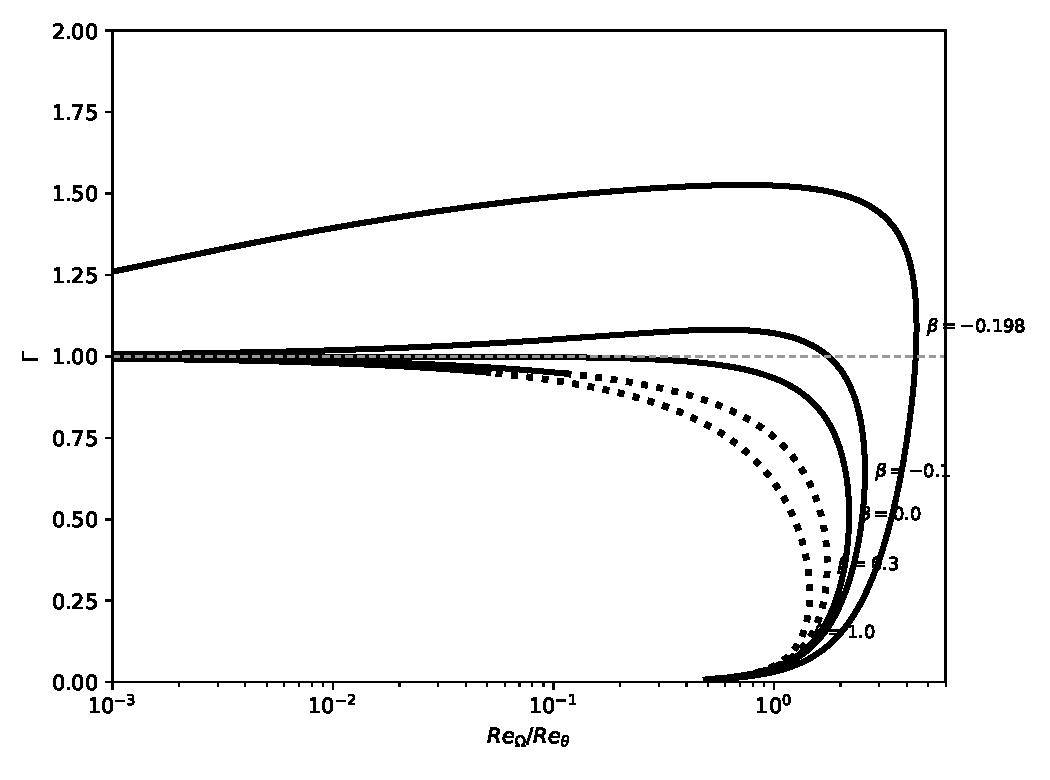
\includegraphics[width=0.72\textwidth]{indicator_plane.pdf}
  \caption{Boundary-layer profiles in the local-indicator plane
  $(Re_\Omega/Re_\theta,\Gamma)$. Each curve is a Falkner--Skan similarity profile
  traced from the wall outward; normalizing $Re_\Omega$ by $Re_\theta$ removes the
  Reynolds number, so the family is universal (the Blasius peak sits at
  $Re_\Omega\!\approx\!2.2\,Re_\theta$). The curves, labeled by $\beta$, span the
  Falkner--Skan family from the adverse separation limit ($\beta\!=\!-0.198$, whose
  $\Gamma$ arches over $1$ into the inflectional range) through Blasius
  ($\beta\!=\!0$) to strong favorable ($\beta\!=\!1$, staying attached at
  $\Gamma\!<\!1$). Line style marks the
  local pressure-gradient parameter: \emph{solid} where $\lambda_p\!<\!0.1$
  (adverse, zero, or mild favorable), \emph{dotted} where $\lambda_p\!\geq\!0.1$
  (strong favorable; $0.1\!\approx\!1/K_\lambda$, the strength at which
  accelerating-flow stabilization becomes significant, Sec.~\ref{sec:calib}).
  Attached profiles reach only $\Gamma\!\approx\!1.5$ even at separation; the fully
  inflectional limit $\Gamma\!\to\!2$ is the detached free shear layer that fixes
  $a_{\max}$ (Sec.~\ref{sec:calib}).}
  \label{fig:indicatorplane}
\end{figure}

The three indicators combine into the single nondimensional rate of
Eq.~\eqref{eq:pai},
\begin{equation}
  a(Re_\Omega,\Gamma,\lambda_p) = a_{\max}\,S(z),
  \quad
  z = s(\Gamma-g_c) + \ln\!\Big(1-\big(Re_\Omega^{\mathrm{c}}(\lambda_p)/Re_\Omega\big)^{p}\Big),
  \quad S(z)=\frac{1}{1+e^{-z}},
  \label{eq:rate}
\end{equation}
with $a\equiv0$ for $Re_\Omega\le Re_\Omega^{\mathrm{c}}$.
The argument $z$ superposes two physically distinct decisions. The
$\Gamma$ term $s(\Gamma-g_c)$ switches amplification on as the profile fills out
toward the inflectional value $\Gamma\!\to\!2$; its center $g_c$ is placed
\emph{above} the attached-layer asymptote $\Gamma\!=\!1$. The design intent
is that the two limits of $\Gamma$ pin the two physical amplification regimes: at
$\Gamma\!=\!2$ the sigmoid is fully on and $a\!\to\!a_{\max}$, the growth rate of a
detached (separated) shear layer, while at $\Gamma\!=\!1$ it is nearly---but
deliberately not fully---off, leaving the small rate at which Tollmien--Schlichting
waves amplify in an attached Blasius boundary layer (the two values are fixed in
Sec.~\ref{sec:calib}). The log-barrier
term is an onset threshold: it drives $z\!\to\!-\infty$ as
$Re_\Omega\!\to\!Re_\Omega^{\mathrm{c}}$ from above and switches off once
$Re_\Omega$ has cleared the cliff, so amplification is forbidden until the layer
is thick enough and then proceeds essentially unattenuated. Two consequences
follow with no added machinery. First, since
$Re_\Omega\!=\!d^2\omega/\nu\!\to\!0$ at the wall, the same threshold suppresses
the viscous sublayer automatically, with no mesh-dependent tuning---there
$\Gamma\!\to\!1$ is a generic near-wall limit, not a true instability. Second---and this is the one modeling decision we make about
pressure gradient---a favorable gradient acts \emph{only} by raising the onset
threshold $Re_\Omega^{\mathrm{c}}(\lambda_p)$ (Eq.~\eqref{eq:cliff_fpg}),
postponing the start of growth; it leaves the growth rate itself untouched. The
$|\mathbf{u}|^2$ denominator of $\lambda_p$ vanishes not only at a stagnation point
but wherever the flow reverses---at separation and reattachment. This is harmless
either way: a favorable-sign $\lambda_p\!\to\!+\infty$ sends
$Re_\Omega^{\mathrm{c}}\!\to\!\infty$ and switches the local rate off (the correct
no-amplification limit), while an adverse-sign $\lambda_p$ is clipped by the
$\max(0,\lambda_p)$ in the cliff and leaves $Re_\Omega^{\mathrm{c}}\!=\!
Re_\Omega^{\mathrm{f}}$ so the rate is set by $\Gamma$, as intended in a separated
shear layer. Since $\lambda_p$ enters only through the exponential of
Eq.~\eqref{eq:cliff_fpg}---nothing ever divides by it---the singular
denominator raises no numerical issue
(the implementation additionally floors $|\mathbf{u}|^2$ at a negligible
value). Both terms read only the local mean flow, never
$\tilde\nu$, so the amplification rate adds no $\tilde\nu$-dependence to the
source linearization. Figure~\ref{fig:kernel} maps the kernel.

\begin{figure}[tp]
  \centering
  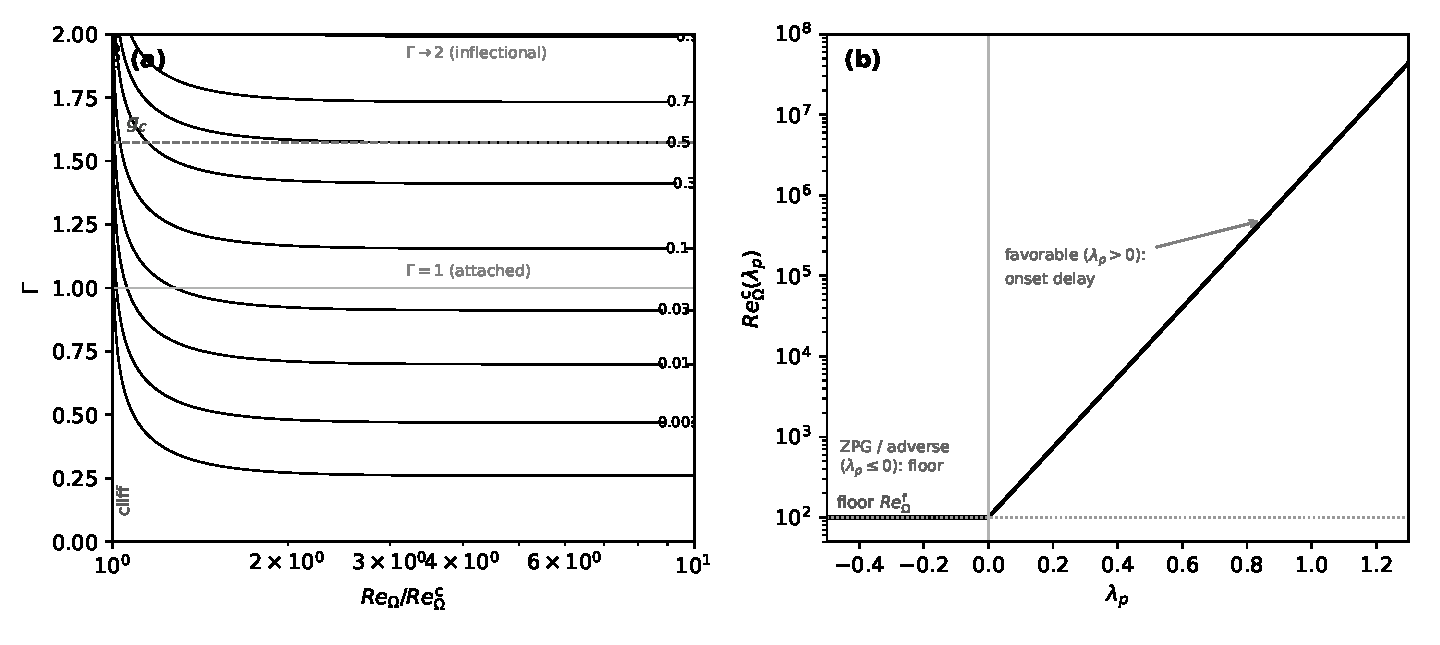
\includegraphics[width=0.98\textwidth]{kernel_maps.pdf}
  \caption{The amplification-rate kernel of Eq.~\eqref{eq:rate}.
  \textbf{(a)} The rate $S(z)$ over the \emph{normalized} vorticity Reynolds
  number $Re_\Omega/Re_\Omega^{\mathrm{c}}$ and the profile-fullness indicator
  $\Gamma$. Because the log barrier depends only on this ratio, the map is
  \emph{universal}: it holds for every pressure gradient, with the onset cliff
  always at $Re_\Omega/Re_\Omega^{\mathrm{c}}\!=\!1$ (dotted). The rate is zero
  left of the cliff, rises as the layer clears it, and---set by the
  $\Gamma$-sigmoid centered at $g_c$ (dashed)---leaves attached profiles
  ($\Gamma\!\approx\!1$) on the low shoulder while saturating on inflectional
  ones ($\Gamma\!\to\!2$). \textbf{(b)} The cliff location
  $Re_\Omega^{\mathrm{c}}(\lambda_p)$ of Eq.~\eqref{eq:cliff_fpg}: a favorable
  gradient ($\lambda_p\!>\!0$) is the only thing that moves the cliff, raising it
  exponentially to delay onset, while zero and adverse gradients rest at the
  floor $Re_\Omega^{\mathrm{f}}$. Together the panels are the complete content of
  the rate---(b) places the cliff, (a) gives the universal shape above it.}
  \label{fig:kernel}
\end{figure}

\paragraph{Favorable-pressure-gradient cliff.} The threshold rises exponentially
with the favorable gradient, so an accelerating layer must grow thicker before
amplification is permitted:
\begin{equation}
  Re_\Omega^{\mathrm{c}}(\lambda_p) =
        Re_\Omega^{\mathrm{f}}\,
        \exp\!\big[K_\lambda\,\max(0,\lambda_p)\big].
  \label{eq:cliff_fpg}
\end{equation}
Here $Re_\Omega^{\mathrm{f}}$ is the cliff floor and $K_\lambda$ the onset-delay
slope. For $\lambda_p\!\le\!0$ (zero or adverse gradient) the threshold sits
exactly at the floor, leaving Blasius and adverse-gradient profiles untouched.
That a favorable gradient should act as an onset delay rather than a change of
growth rate is itself a claim about stability theory---one that lets the slope be
anchored to the $e^N$ critical Reynolds number rather than tuned freely; we make
the argument precise, and fix $K_\lambda$ and $Re_\Omega^{\mathrm{f}}$, in
Sec.~\ref{sec:calib}.

Equation~\eqref{eq:pai} grows $\tilde\nu$ along the flow at the local rate
$a\,\omega$, so $\ln(\tilde\nu/\tilde\nu_\infty)$ accumulates monotonically in the
manner of an amplification factor $N$; because $a_{\max}$ is small
(Sec.~\ref{sec:calib}) the accumulation is gentle and targets the onset
location rather than matching the $e^N$ growth rate quantitatively. Transition is
reached when $\tilde\nu$ has grown to $\chi\sim1$, where the eddy viscosity becomes
dynamically active.

\subsection{One-equation blend}
A handover weight ties the laminar and turbulent regimes to the single state
variable through $\chi$,
\begin{equation}
  \sigma_t(\chi;\tau) = \max\!\left[\,1-e^{-(\chi-1)/\tau},\;0\right] \;=\;
  \begin{cases} 0, & \chi \le 1, \\ 1-e^{-(\chi-1)/\tau}, & \chi > 1. \end{cases}
  \label{eq:sigma}
\end{equation}
The
production and destruction of Eq.~\eqref{eq:sa} are blended, each with its own
width,
\begin{equation}
  P = \max\!\big[(1-\sigma_P)\,P_\mathrm{AI},\;\sigma_P\,P_\mathrm{SA}\big], \qquad
  D = \sigma_D\,D_\mathrm{SA}, \qquad
  \sigma_P = \sigma_t(\chi;\tau), \quad \sigma_D = \sigma_t(\chi;\tau_D).
  \label{eq:blend}
\end{equation}
The $\max$ hands the production cleanly from amplification to SA at the
crossover: for $\chi\!\le\!1$ ($\sigma_P\!=\!0$) it returns $P_\mathrm{AI}$,
leaving the $e^N$ amplification unchanged, and once $\sigma_P P_\mathrm{SA}$
overtakes it just past $\chi\!=\!1$ the source reverts to standard SA with no
laminar residue (a pressure-sensitive residue left past $\chi\!=\!1$ would couple
the transition front to the outer pressure field; Sec.~\ref{sec:blendnlf}).
Gating the destruction is likewise
essential, since the SA wall-damping destruction would otherwise quench the
gentle amplification; both gates vanish for $\chi\!\le\!1$, so the
laminar range sees no destruction at any width. The destruction gate opens
faster ($\tau_D\!<\!\tau$): equal widths would leave a small surplus of
$\tilde\nu$ in the turbulent buffer layer, where both sources run throttled;
Sec.~\ref{sec:calib_diff} chooses $\tau_D$ to cancel it, making the fully
turbulent log law match standard SA exactly. The limit
$\sigma_t\!\to\!1$ recovers the unmodified SA
equation and its fully turbulent calibration.
\subsection{Cross-stream diffusion of the laminar disturbance}\label{sec:nulamscale}
The SA diffusion operator is retained in both regimes, but its molecular
coefficient must be reduced for the laminar amplification to survive. We scale
the laminar viscosity in the SA diffusion term---and only there---by a constant
factor $c_{\nu,\mathrm{ai}}\!<\!1$,
\begin{equation}
  (\nu+\tilde\nu)\;\longrightarrow\;(c_{\nu,\mathrm{ai}}\,\nu+\tilde\nu)
  \quad\text{in the diffusion term of Eq.~\eqref{eq:sa} only,}
  \label{eq:nulamscale}
\end{equation}
leaving the mean-flow viscosity, the SA production and destruction, and the
definition $\chi=\tilde\nu/\nu$ (formed with the \emph{true} $\nu$) untouched.
Only the molecular coefficient is scaled: relative to it, the nonlinear
self-diffusion $\tilde\nu\,\nabla^2\tilde\nu$ and the $c_{b2}|\nabla\tilde\nu|^2$
gradient term are both smaller by a factor $O(\chi)$ and hence
negligible where $\chi\!\ll\!1$, so we leave them as in Eq.~\eqref{eq:sa}.

The reduction is needed because, while the disturbance is sub-$O(1)$
($\chi\!<\!1$), the diffusion coefficient $(\nu+\tilde\nu)$ is dominated by the
molecular part $\nu$, which does not vanish as the working variable does. In a
thin, low-$Re_\theta$ laminar layer the amplifying band is narrow and abuts the
$\tilde\nu\!=\!0$ wall condition, so with the full molecular coefficient the
cross-stream smearing drains the disturbance as fast as the gentle rate
$a\,\omega$ grows it, and transition never occurs. The drain is also
uneven: relative to the growth it scales like $1/Re_\theta$, hitting thin
layers hardest and bending the envelope away from the $e^N$ form. Reducing the molecular
coefficient keeps the in-BL $\tilde\nu$ peak co-located with the $Re_\Omega$
peak; the value of $c_{\nu,\mathrm{ai}}$ is determined in
Sec.~\ref{sec:calib_rate}.

This reduction leaves Spalart's turbulent calibrations intact; the
region-by-region accounting, verified against a wall-layer solve, is likewise
deferred to Sec.~\ref{sec:calib_diff}.

\section{Determination of model constants}\label{sec:calib}

The constants are fixed in the order the physics permits, each at a
canonical limit rather than against the transition cases that follow. The
free-shear ceiling $a_{\max}$ stands alone and is fixed first. The next
three---the sigmoid pair $(s,g_c)$, the diffusion reduction
$c_{\nu,\mathrm{ai}}$, and the onset floor $Re_\Omega^{\mathrm{f}}$---cannot
be set independently and are fixed together against the Blasius $e^N$
envelope (Sec.~\ref{sec:calib_rate}). The favorable-gradient slope
$K_\lambda$ then follows from the rate at which Drela's critical Reynolds
number rises with pressure gradient (Sec.~\ref{sec:calib_klambda},
Eq.~\eqref{eq:klambda}). The handover widths are fixed last, on the fully
turbulent wall layer, where the requirement is invariance: the modifications
must vanish outside a thin buffer band, and with the calibrated $\tau_D$
they do (Sec.~\ref{sec:calib_diff}). The freestream seed
(Sec.~\ref{sec:calib_tu}) closes the set. The airfoil cases therefore remain
predictive tests.\footnote{In the manner of Zhuangzi's cook
(\begin{CJK}{UTF8}{bsmi}庖丁解牛\end{CJK}), whose blade stays sharp for
nineteen years because it passes only through the openings the ox already
has: each constant sits at a joint the physics provides.}

\subsection{The rate ceiling and the attached-layer calibration}\label{sec:calib_rate}

The magnitude $a_{\max}$ is the free-shear amplification ceiling. The sigmoid
saturates ($S\!\to\!1$) as $\Gamma\!\to\!2$, the value a fully inflectional
profile reaches---the detached shear layer over a laminar separation bubble.
There the instability is the inviscid Rayleigh/Kelvin--Helmholtz mode of a free
shear layer, whose maximum growth rate scaled by the local vorticity is a
classical $O(0.15$--$0.2)$~\cite{michalke_1964}: for the canonical
hyperbolic-tangent mixing layer the most-amplified temporal mode grows at
$\omega_{i,\max}\!\approx\!0.19\,U_0/\delta$ against a peak vorticity
$\omega_\mathrm{peak}\!=\!U_0/\delta$. We identify $a_{\max}$
with this free-shear ceiling and set $a_{\max}\!=\!0.15$, at the low end of the
range: a wall-bounded separated layer grows somewhat more slowly than an ideal
free mixing layer, and the rate is deliberately gentle (Sec.~\ref{sec:model}).

The next three constants---the sigmoid pair $(s,g_c)$, the diffusion
reduction $c_{\nu,\mathrm{ai}}$, and the onset floor
$Re_\Omega^{\mathrm{f}}$---are coupled: on an attached layer the observable
is the \emph{net} envelope, amplification $a\,\omega$ minus the cross-stream
drain, permitted only above the floor. All three shape one curve,
$N(Re_\theta)$ on the Blasius layer, and are set together against it.

With the ceiling fixed at $\Gamma\!=\!2$, the pair $(s,g_c)$ sets how far the rate
is throttled at the attached-layer value $\Gamma\!=\!1$---the wall asymptote
($\omega d/|\mathbf{u}|\!\to\!1$) of any attached zero- or favorable-pressure-gradient
layer. Because $a\,\omega$
integrates along the layer to $N$ (Sec.~\ref{sec:model}), the
throttled value $a(\Gamma\!=\!1)$ controls the flat-plate envelope slope
$dN/dRe_\theta$. We place $g_c$ between the attached ($\Gamma\!=\!1$) and
inflectional ($\Gamma\!=\!2$) limits and set the slope $s$ so that
$a(\Gamma\!=\!1)\!=\!0.007$ reproduces Drela's Blasius envelope
($dN/dRe_\theta$ of order $10^{-2}$~\cite{drela_giles_1987}), fixing
$(s,g_c)\!=\!(5.263,1.572)$. The center sits near $g_c\!\approx\!1.5$ because requiring the
sigmoid fully on at $\Gamma\!=\!2$ and barely on at
$\Gamma\!=\!1$ forces it roughly midway between the two; the pair was tuned
only against these two anchors.

The $\Gamma$-independent cliff floor is set at $Re_\Omega^{\mathrm{f}}\!=\!100$.
Through the Blasius relation $\max_y Re_\Omega\!\approx\!2.2\,Re_\theta$ this is a
\emph{soft} gate at $Re_\theta\!\approx\!45$---well below Drela's
$Re_{\theta,\mathrm{crit}}\!\approx\!200$. The low value is deliberate: the
floor merely \emph{permits} amplification, which the log-barrier
and the gentle rate hold negligible until the layer is well past the cliff, so
the \emph{appreciable} growth of $\tilde\nu$ sets in near
$Re_{\theta,\mathrm{crit}}$, as the coupled flat plate confirms
(Sec.~\ref{sec:flatplate}). The floor is pushed below the nominal critical
threshold to offset the reduced-but-nonzero laminar diffusion
(Sec.~\ref{sec:nulamscale}) that otherwise damps the sub-$O(1)$ disturbance.
The round value is not carefully tuned; future work may place the floor
better.
A single, gradient-independent floor suffices, because the pressure-gradient
dependence of \emph{onset} is already carried by $Re_\Omega$ itself. Adverse
layers transition earliest---Drela's critical $Re_\theta$ falls as the shape
factor $H$ rises---and they are also the fullest in vorticity: at a given
$Re_\theta$ a high-$H$ profile carries a larger $Re_\Omega/Re_\theta$ than Blasius
(Fig.~\ref{fig:indicatorplane}), so it clears the fixed floor at a \emph{lower}
$Re_\theta$ with no adjustment to the cliff. The sensor $\lambda_p$ is thus left a
single job---raising $Re_\Omega^{\mathrm{c}}$ in \emph{favorable} gradients
(Eq.~\eqref{eq:cliff_fpg}) to delay onset there.

The joint fit is made on the Blasius layer, where the working
variable can be watched behaving as an amplification factor. We solve the
disturbance transport equation in
non-dimensional boundary-layer variables (length in $\nu/U_\infty$, velocities
normalized by $U_\infty$),
\begin{equation}
  u\,\frac{\partial\hat\nu}{\partial x} + v\,\frac{\partial\hat\nu}{\partial y}
  = \frac{c_{\nu,\mathrm{ai}}}{\sigma_\mathrm{SA}}\,\frac{\partial^2\hat\nu}{\partial y^2}
    + a(Re_\Omega,\Gamma)\,\omega\,\hat\nu,
  \label{eq:transport}
\end{equation}
using the same SA cross-stream diffusion as the coupled model---coefficient
$\sigma_\mathrm{SA}\!=\!2/3$ with the reduced laminar scale
$c_{\nu,\mathrm{ai}}\!=\!1/12$ (determined here)---on the Blasius layer, seeded
with $\hat\nu_\infty\!=\!1$ at the leading edge as a unit-scale reference, so that
$N\!=\!\ln(\hat\nu/\hat\nu_\infty)\!=\!\ln\hat\nu$ is the amplification factor by
construction. Figure~\ref{fig:nuhat}(a) shows $\ln\hat\nu$ growing monotonically
from the seed, concentrated in the unstable band between $\theta$ and
$\delta_{99}$, and accumulating to $N\!\approx\!14$ over the
$Re_x\!\le\!4\!\times\!10^6$ ($Re_\theta\!\le\!1328$) plate: the working variable
acts as an envelope amplification factor spanning the range required for natural
transition. Panel (b) re-plots the solution as the envelope $\max_y\hat\nu$
versus $Re_\theta$, against the Drela--Giles Blasius envelope---zero to
$Re_{\theta,\mathrm{crit}}\!=\!242$, then slope
$1.04\!\times\!10^{-2}$~\cite{drela_giles_1987}: the computed envelope is
drained below the correlation early, steepens past it late, and reaches
$N\!=\!9$ within $10\%$ of it. A physical case seeded with $\chi_\infty$ reaches the handover where
the envelope crosses $N_\mathrm{crit}\!=\!\ln(c_{v1}/\chi_\infty)$---the
half-saturation threshold $\chi\!=\!c_{v1}$ at which the eddy viscosity engages;
the $C_f$ rise begins $\ln c_{v1}\!\approx\!2$ $e$-folds earlier, at
$\chi\!=\!1$. The seed is well posed as an inflow
condition: in the irrotational outer flow the production vanishes with the
vorticity and the destruction is gated off in the laminar range ($\sigma_D\!=\!0$
for $\chi\!\le\!1$), so $\chi_\infty$ is convected essentially undisturbed from the
inflow to the leading edge---a fixed, location-independent amplitude, unlike a
freestream closure that decays along the domain.
The coefficient $c_{\nu,\mathrm{ai}}\!=\!1/12$ is itself fixed by this
solution. With the unmodified value
($c_{\nu,\mathrm{ai}}\!=\!1$) the molecular diffusion of the sub-$O(1)$
$\tilde\nu$ over-damps the gentle amplification and the envelope collapses to
$N\!\approx\!2$, suppressing transition; $c_{\nu,\mathrm{ai}}\!=\!1/4$ is still
too diffusive to recover it; $c_{\nu,\mathrm{ai}}\!=\!1/12$ restores a
$dN/dRe_\theta$ in the Drela envelope range ($N\!\approx\!14$). It is a round
value chosen for adequacy, and more careful tuning is left to future work.

\begin{figure}[tp]
  \centering
  
\includegraphics[width=0.99\textwidth]{blasius_nuHat_solution.pdf}
  \caption{The attached-layer calibration, verified on the Blasius layer:
  disturbance transport \eqref{eq:transport} with the jointly set $(s,g_c)$,
  $c_{\nu,\mathrm{ai}}$, and $Re_\Omega^{\mathrm{f}}$
  ($\hat\nu_\infty\!=\!1$ seed, $a_{\max}\!=\!0.15$). \textbf{(a)}
  Contours of $N\!=\!\ln\hat\nu$ in the $(Re_x,Re_y)$ plane: the working
  variable grows monotonically as an envelope amplification factor, reaching
  $N\!\approx\!14$ over the $Re_x\!\le\!4\!\times\!10^6$
  ($Re_\theta\!\le\!1328$) plate, concentrated between the overlaid
  momentum thickness $\theta$ and edge thickness $\delta_{99}$, where
  $Re_\Omega$ peaks. \textbf{(b)} The same solution as the envelope
  $\max_y\hat\nu$ vs $Re_\theta$ (log left axis; $N$ linear right axis)
  against the Drela--Giles Blasius envelope~\cite{drela_giles_1987}---zero
  to $Re_{\theta,\mathrm{crit}}\!=\!242$, then slope
  $1.04\!\times\!10^{-2}$: drained below the correlation early, steeper
  late, reaching $N\!=\!9$ within $10\%$. A physical case seeded with
  $\chi_\infty$ hands over where this envelope crosses
  $N_\mathrm{crit}\!=\!\ln(c_{v1}/\chi_\infty)$ ($\chi\!=\!c_{v1}$).}
  \label{fig:nuhat}
\end{figure}

The response at intermediate fullness was not itself calibrated, so it is a
genuine---and absolute---test. For each Falkner--Skan profile we march the
same transport \eqref{eq:transport} on the similarity field, exactly as for
the Blasius layer of Fig.~\ref{fig:nuhat}. The slope $dN/dRe_\theta$ is not one
number: the diffusion-to-growth ratio decays like $1/Re_\theta$, so
$N(Re_\theta)$ is convex and the local rate rises along the layer. We
therefore report two measures per profile: the onset-to-transition
\emph{mean}---$N\!=\!9$ over the run from the cliff-floor crossing
$Re_\theta^{\mathrm{c}}$ to $Re_\theta(N{=}9)$---which is what sets the
transition location, and the \emph{late} rate---the $N\!\in\![5,9]$
secant---to which the local slope has risen as transition
nears.\footnote{Numerics as for
Fig.~\ref{fig:nuhat}: implicit march in $x$, reduced diffusion
$c_{\nu,\mathrm{ai}}/\sigma$, seed $\hat\nu_\infty\!=\!1$, on the wedge field
$U_e\!\propto\!x^{m}$, $m\!=\!\beta/(2-\beta)$; the kernel runs at
$\lambda_p\!=\!0$, so the cliff sits at its floor.
$Re_\theta^{\mathrm{c}}$ is $Re_\Omega^{\mathrm{f}}$ divided by the
profile's peak $Re_\Omega/Re_\theta$ ratio. Domains are sized so $N$ reaches
$\approx\!14$; slopes are grid-converged to under $2\%$.}
Figure~\ref{fig:shapefactor} compares both to the Drela--Giles
envelope-rate correlation $dn/dRe_\theta(H)$ with \emph{no normalization}.
At Blasius the mean is $9.4\!\times\!10^{-3}$ against the correlation's
$1.04\!\times\!10^{-2}$ ($-9\%$), the late rate $1.48\!\times\!10^{-2}$
($+43\%$). From Blasius to the separation limit ($H\!=\!2.59$--$3.64$) the
late rate follows the correlation's order-of-magnitude rise to within
$-15/{+}43\%$---within $\pm10\%$ over the mid-adverse branch---while the
mean runs $0.6$--$0.9\times$: the single-valued correlation runs along the
band the two measures span, at or just above its upper edge over the
mid-adverse branch and descending to the mean at Blasius, cross-stream
diffusion and layer-wide interaction included. On the favorable side both
measures deliberately do not drop with the correlation:
favorable-gradient stabilization enters the model through the
onset-delay cliff (Sec.~\ref{sec:calib_klambda}), not the growth rate
(Sec.~\ref{sec:model}). The residual mismatch also bounds what further
tuning could buy: the logistic form of the sigmoid was adopted for
smoothness, not derived, and neither it nor alternative kernel shapes were
investigated beyond the two anchors---future work on the kernel's form may
increase the fidelity of this comparison.

\begin{figure}[tp]
  \centering
  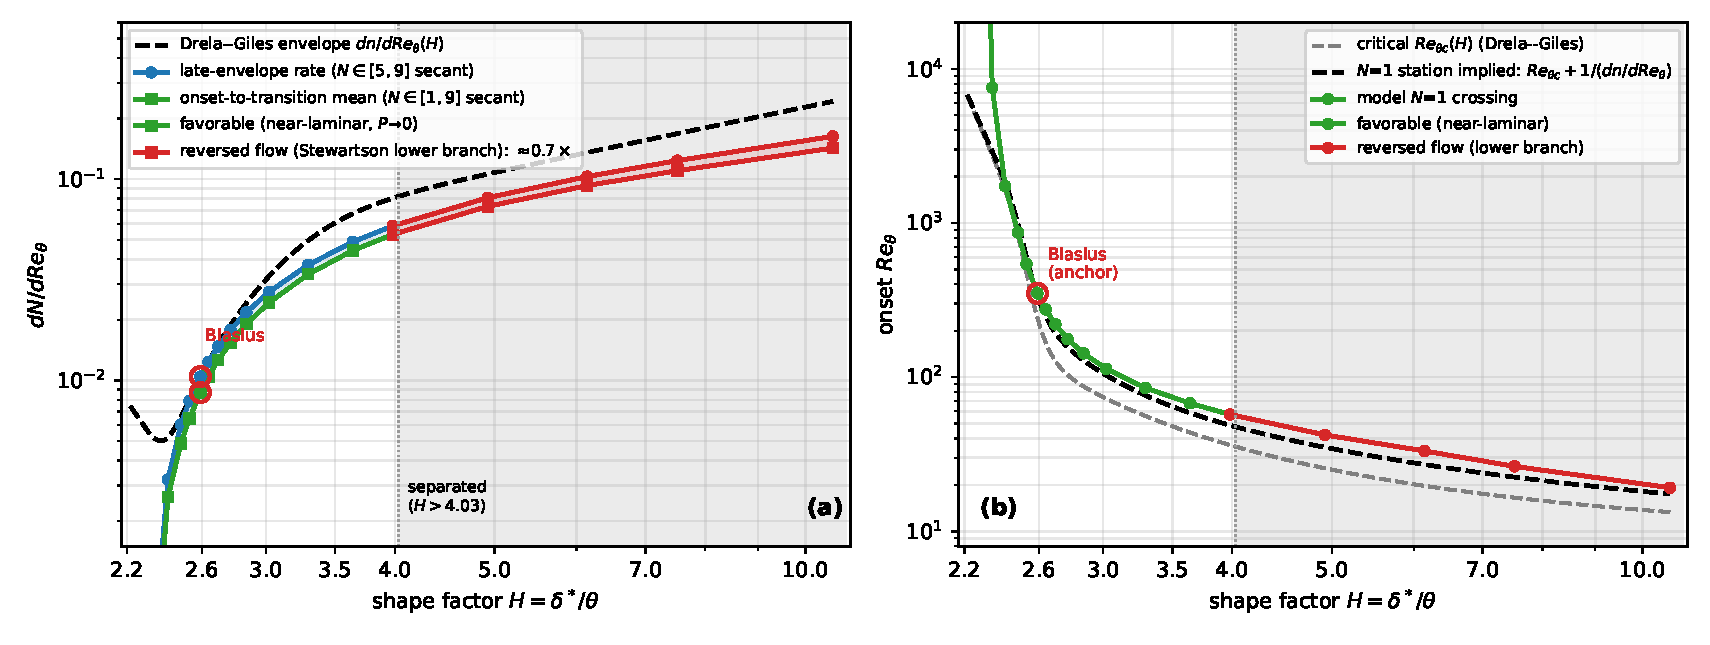
\includegraphics[width=0.58\textwidth]{shapefactor_amplification.pdf}
  \caption{Shape-factor dependence of the envelope rate, compared
  \emph{absolutely}---no normalization constant. For each Falkner--Skan
  profile the disturbance transport \eqref{eq:transport} is marched on the
  similarity field exactly as for the Blasius layer of Fig.~\ref{fig:nuhat};
  because the local slope rises along the layer as the diffusion deficit
  fades, two measures are shown: the onset-to-transition mean (squares,
  $Re_\theta^{\mathrm{c}}\!\to\!N\!=\!9$) and the late-envelope rate
  (circles, $N\!\in\![5,9]$ secant), the band between them shaded. Over the
  zero-to-adverse branch (filled symbols) the Drela--Giles
  correlation~\cite{drela_giles_1987} runs along this band across its
  order-of-magnitude rise; toward separation (shaded region) the sigmoid
  saturates to the free-shear ceiling $a_{\max}$. On the favorable branch
  (open symbols) the rate deliberately does not follow the correlation's
  drop: favorable-gradient stabilization enters through the onset-delay
  cliff (Sec.~\ref{sec:calib_klambda}), not the rate. Blasius (red rings) is
  the anchor of Sec.~\ref{sec:calib_rate}.}
  \label{fig:shapefactor}
\end{figure}

\subsection{Favorable-gradient onset delay}\label{sec:calib_klambda}

The favorable-gradient onset-delay slope $K_\lambda$ follows from the same
anchoring logic, once one asks \emph{where} on a profile growth is triggered.
The cliff is applied pointwise, so amplification is permitted wherever the local
$Re_\Omega$ clears its local threshold $Re_\Omega^{\mathrm{c}}(\lambda_p)$; growth
therefore triggers at the \emph{worst} point---the wall-normal location that
maximizes $Re_\Omega/Re_\Omega^{\mathrm{c}}$ (equivalently, the largest local rate
$S$). There is no single $\lambda_p$ for a profile: on a favorable-gradient layer
the $Re_\Omega$ peak sits in the outer boundary layer, where $\lambda_p$ is large
and the cliff is high, so the trigger retreats inboard to where $\lambda_p$ is
small. Figure~\ref{fig:worstpoint} places Falkner--Skan profiles, from adverse
through strong favorable gradient, each at its Drela--Giles critical Reynolds
number $Re_{\theta c}(H)$, in the $(Re_\Omega,\Gamma)$ plane, colored by the local
rate $S$ the solver computes; the star marks the worst (triggering) point.
Adverse profiles arch over $\Gamma\!=\!1$ into the inflectional, strongly
amplifying band and ignite hard at low $Re_\theta$; favorable profiles stay at
$\Gamma\!<\!1$ and ignite only weakly, at a worst point close to the wall.

\begin{figure}[tp]
  \centering
  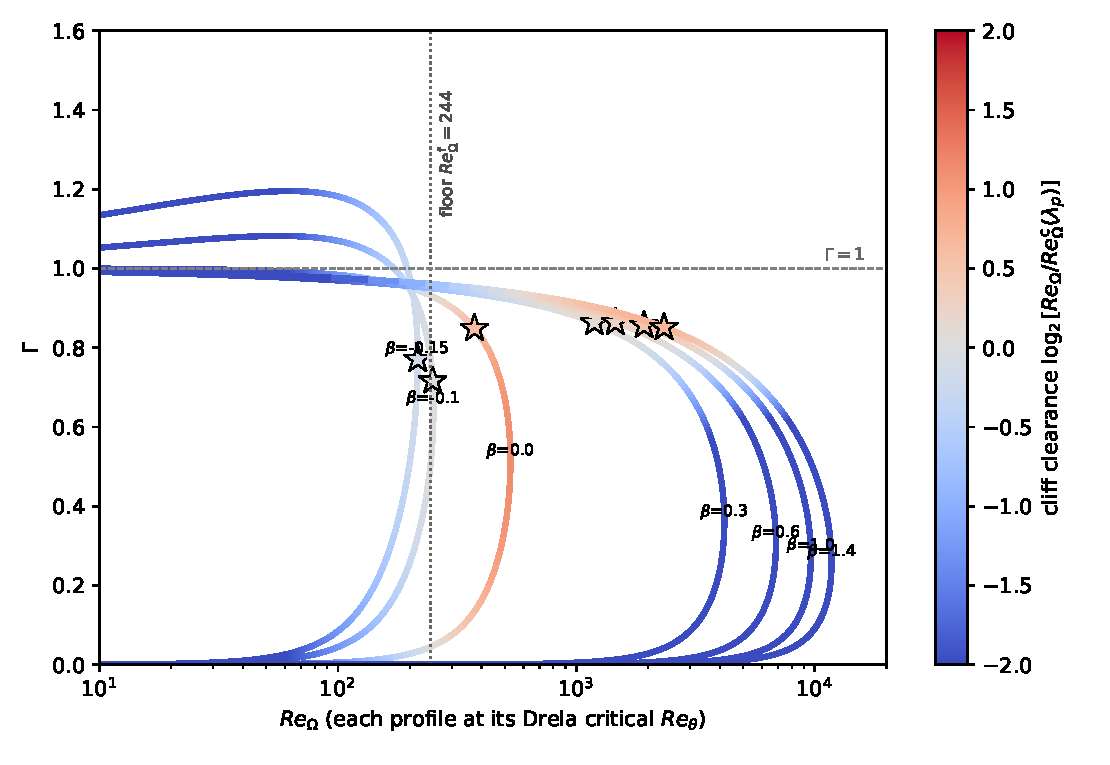
\includegraphics[width=0.72\textwidth]{klambda_profiles.pdf}
  \caption{Where growth is triggered. Falkner--Skan profiles---adverse
  ($\beta\!<\!0$) through strong favorable ($\beta\!=\!1.4$)---each at its own
  Drela--Giles critical Reynolds number $Re_{\theta c}(H)$, in the true
  $(Re_\Omega,\Gamma)$ plane, colored by the local amplification rate $S$; the
  star on each is the \emph{worst} (triggering) point, $\max_\eta S$. Adverse
  profiles arch over $\Gamma\!=\!1$ into the inflectional band and ignite hard;
  favorable profiles stay below $\Gamma\!=\!1$ and ignite weakly, with the trigger
  driven toward the wall (small $\lambda_p$). The low-$Re_\theta$ Blasius star is
  slightly hotter than the favorable ones---see text.}
  \label{fig:worstpoint}
\end{figure}

The sensitivity of the worst $\lambda_p$ to $\beta$ pins $K_\lambda$. As the
gradient turns weakly favorable ($\beta\!\to\!0^+$), the worst point's $\lambda_p$
rises at a rate $d\lambda_p^{\mathrm{worst}}/d\beta\!\approx\!1.3$ (at
$K_\lambda\!=\!10$); the trigger's inboard
retreat holds this slope well below the $\approx\!2$ of the $Re_\Omega$-peak
$\lambda_p$ (using the peak value instead is what makes a naive estimate come out
several times too small). Over the same range Drela's critical Reynolds number
climbs steeply, $d\ln Re_{\theta c}/d\beta=(d\ln Re_{\theta c}/dH)(dH/d\beta)
\approx(-11.2)(-1.09)\approx 12.3$. Requiring the cliff to lift the onset
threshold at exactly the rate the critical Reynolds number
rises~\cite{drela_giles_1987} gives
\begin{equation}
  K_\lambda = \left.\frac{d\ln Re_{\theta c}/d\beta}{d\lambda_p^{\mathrm{worst}}/d\beta}\right|_{\beta\to0}
  \approx \frac{12.3}{1.3} \approx 9.5.
  \label{eq:klambda}
\end{equation}
The denominator---the worst-point slope---itself depends on the $K_\lambda$ used
to locate the worst point, so Eq.~\eqref{eq:klambda} is a self-consistency
condition rather than a closed form. It settles quickly: evaluated at
$K_\lambda\!=\!5$, $9$, and $10$, the right-hand side returns $12.6$, $10.0$, and
$9.5$, so input and output cross near $K_\lambda\!\approx\!9.7$. We adopt the round
value $K_\lambda\!=\!10$; a more careful calibration is left to future work.

A corollary is visible in Figure~\ref{fig:worstpoint}: the low-Reynolds Blasius
profile ignites at slightly \emph{higher} $S$ than the accelerated ones. This is
consistent with the reduced laminar diffusion---Blasius transitions at small
$Re_\theta$, where the thin layer makes the residual $c_{\nu,\mathrm{ai}}\nu$
diffusion relatively stronger, so a little more amplification is needed for net
growth, while favorable layers transition at much larger $Re_\theta$ and need
less.

\subsection{The turbulent layer and the handover}\label{sec:calib_diff}


What remains is the turbulent side: the reduced diffusion and the two gates
must leave SA's calibrated behavior alone. This subsection shows that they
do---the diffusion reduction exactly, everywhere; the gates within a thin
buffer band---and then chooses the destruction width $\tau_D$ to cancel the
gates' one observable consequence there.

The diffusion reduction is invisible to Spalart's turbulent calibrations for
a structural reason: $c_{\nu,\mathrm{ai}}$ rescales
only the \emph{molecular} part of the diffusion, which is appreciable relative to
$\tilde\nu$ only in the sub-$O(1)$ range that SA leaves inert---the very range the
model repurposes---and is negligible wherever the turbulent calibrations act.
Those constants ($c_{b1},c_{b2},c_{w1},\sigma,\kappa,c_{v1}$) were fixed on
high-Reynolds turbulent flows---free-shear spreading rates and flat-plate skin
friction---and the scaling \eqref{eq:nulamscale} leaves each intact, as a
region-by-region partition confirms:
\begin{enumerate}
  \item \emph{Outer layer, wakes, and mixing layers (asymptotic dominance).}
  Wherever these calibrations act, $\tilde\nu\!\gg\!\nu$ ($\chi\!\gtrsim\!100$),
  so $c_{\nu,\mathrm{ai}}\nu+\tilde\nu\!\approx\!\tilde\nu\!\approx\!\nu+\tilde
  \nu$; dividing an already sub-percent molecular contribution by twelve is
  imperceptible, and spreading rates and the outer velocity deficit are
  unchanged.
  \item \emph{Viscous sublayer (exact zero-curvature).} At the wall $\tilde\nu$
  is linear, $\tilde\nu\!\to\!a\,y$; the SA constant
  $c_{w1}\!=\!c_{b1}/\kappa^2+(1+c_{b2})/\sigma$ balances the quadratic
  production, destruction, and self-diffusion so that the \emph{linear} molecular
  diffusion is the surviving near-wall constraint,
  $(c_{\nu,\mathrm{ai}}\nu/\sigma)\,\partial^2\tilde\nu/\partial y^2\!=\!0$.
  Because $c_{\nu,\mathrm{ai}}\nu$ is a nonzero constant it still enforces
  $\partial^2\tilde\nu/\partial y^2\!=\!0$: the scaling multiplies a term that
  evaluates to zero and cannot alter the sublayer profile.
  \item \emph{Buffer layer (shielded by $f_{v1}$).} The lone region where
  $\nu\!\sim\!\tilde\nu$ is the buffer layer, and there the change is only a
  $\sim\!15\%$ local reduction in diffusion (at $\chi\!\approx\!5$,
  $(\tfrac{1}{12}+5)/(1+5)\!\approx\!0.85$). Since $\chi$ is formed with the true
  $\nu$, the damping function $f_{v1}\!=\!\chi^3/(\chi^3+c_{v1}^3)$
  ($c_{v1}\!=\!7.1$) still switches on the eddy viscosity at exactly the
  calibrated $\chi$; it absorbs most of the resulting $\tilde\nu$ perturbation
  before it reaches $\nu_t\!=\!\rho\tilde\nu f_{v1}$, the quantity the momentum
  equations feel.
\end{enumerate}
A constant-stress wall-layer solve makes the accounting quantitative. Integrating
the SA transport in wall units with the reduced coefficient acting alone
($c_{\nu,\mathrm{ai}}\!=\!1/12$, gates held at $\sigma_P\!=\!\sigma_D\!\equiv\!1$) leaves the
computed log-law intercept unchanged to within $10^{-3}$: the molecular term is
subdominant in the $\tilde\nu$ balance even through the buffer layer, so the
$\tilde\nu$ profile---and with it $\nu_t$---is unmoved by even a twelvefold
reduction of the molecular coefficient (Fig.~\ref{fig:walllayer}).

The handover introduces two coefficients of its own, the production and
destruction widths $\tau$ and $\tau_D$ of Eq.~\eqref{eq:blend}. The production
width is set \emph{ab initio} rather than
by tuning: the handoff begins as soon as $\chi$ exceeds $1$---where $\tilde\nu$
starts to feed the eddy viscosity---and should be largely complete by the scale
$\chi\!\sim\!c_{v1}$ at which $f_{v1}$ reaches half saturation
($\sigma_P\!=\!0.78$ there), a span that $\tau\!=\!4$ realizes. The destruction
width is then fixed by one more canonical anchor---the fully turbulent log law
itself---as follows.

Gating production and destruction by a \emph{common} weight would leave a
turbulent-wall footprint: the one place the gates, rather than the diffusion,
touch SA's calibration. The weight approaches unity only for
$\chi\!\gtrsim\!20$ ($y^+\!\gtrsim\!50$, where $\chi\!\approx\!\kappa y^+$), so the SA
production and destruction run partially throttled through the buffer layer; there
the disturbance branch $P_\mathrm{AI}$ is already extinct ($\Gamma\!\to\!0$,
$Re_\Omega\!<\!Re_\Omega^{\mathrm{f}}$), so the blend has fully reverted to SA and
the gates merely scale the recovered SA source. On the log-law solution,
production and destruction do not balance each other---$P/D =
c_{b1}/(c_{w1}\kappa^2)\!\approx\!1/4$, diffusion supplying the
difference---so throttling both by the \emph{same} factor would leave a net
positive
residual, $(1-\sigma_t)(1+c_{b2})\kappa^2 u_\tau^2/\sigma$, and with it a
spurious buffer-layer surplus of $\tilde\nu$ that depresses the log-law
intercept. The separate destruction width
absorbs exactly this residual: opening the destruction gate faster restores the
buffer balance, and requiring the computed log law
to match standard SA fixes
$\tau_D\!=\!1.36$. The calibrated model's intercept shift is below $10^{-3}$
and its peak buffer-layer
eddy-viscosity perturbation is $0.8\%$
(Fig.~\ref{fig:walllayer}).

Does the modification change SA's tolerance to
\emph{coarse} near-wall meshes---SA's practical advantage over two-equation models,
which typically require $y^+\!\lesssim\!1$? Solving the same wall-layer equations on
grids whose first node is progressively coarsened (first-cell $y^+$ from $0.25$ to
$8$, geometric growth to the edge) answers this (Table~\ref{tab:yplus}).
The grid-induced skin-friction error is indistinguishable between standard SA and
SA-AI at every resolution: both hold $C_f$ to within $0.5\%$ at first-cell
$y^+\!=\!2$ and $\sim\!1\%$ at $y^+\!=\!4$, degrading to a few percent only by
$y^+\!=\!8$; and with the calibrated $\tau_D$ the recovered intercept matches
standard SA's to within $0.01$ throughout. SA-AI
inherits SA's coarse-mesh robustness intact.

\begin{table}[tp]
  \centering
  \small
  \caption{Coarse-mesh robustness. The constant-stress wall-layer equations are
  solved with a second-order finite-difference scheme on grids whose first node
  sits at the listed first-cell $y^+$ (geometric growth ratio $1.2$ to the edge
  $y^+\!=\!1000$; total node count in the second column), for standard SA and
  SA-AI. Columns give the recovered log-law intercept $B$ and the grid-induced
  skin-friction error $|\Delta C_f/C_f|$ relative to the finest grid. SA-AI's grid
  sensitivity matches standard SA's at every resolution, and with the calibrated
  destruction width $\tau_D$ its intercept matches standard SA's.}
  \label{tab:yplus}
  \begin{tabular}{cc cc cc}
    \toprule
    & & \multicolumn{2}{c}{standard SA} & \multicolumn{2}{c}{SA-AI}\\
    \cmidrule(lr){3-4}\cmidrule(lr){5-6}
    first-cell $y^+$ & nodes & $B$ & $|\Delta C_f/C_f|$ & $B$ & $|\Delta C_f/C_f|$\\
    \midrule
    0.25 & 38 & 5.16 & ref    & 5.16 & ref \\
    0.5  & 34 & 5.17 & 0.1\%  & 5.17 & 0.1\% \\
    1    & 31 & 5.18 & 0.2\%  & 5.18 & 0.2\% \\
    2    & 27 & 5.21 & 0.4\%  & 5.21 & 0.4\% \\
    4    & 23 & 5.26 & 0.9\%  & 5.27 & 1.0\% \\
    8    & 19 & 5.44 & 2.5\%  & 5.44 & 2.6\% \\
    \bottomrule
  \end{tabular}
\end{table}

\begin{figure}[tp]
  \centering
  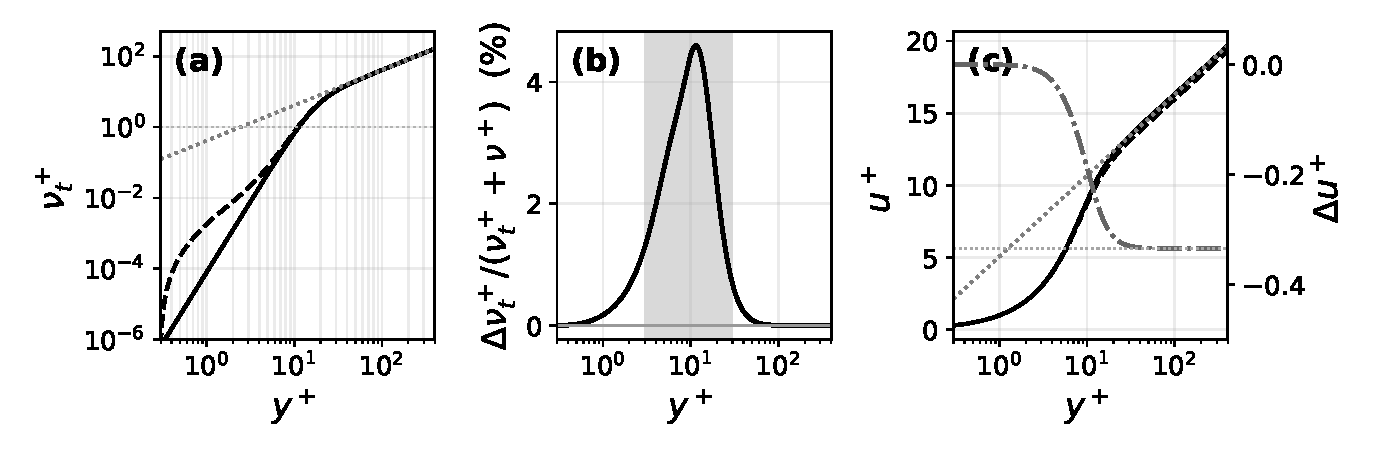
\includegraphics[width=0.98\textwidth]{wall_layer.pdf}
  \caption{Footprint of the SA-AI modifications on a fully turbulent
  constant-stress wall layer, from the SA transport solved in wall units
  ($\chi\!=\!\kappa y^+$). \textbf{(a)} Eddy viscosity $\nu_t^+$ for original SA
  (solid) and SA-AI (dashed, $\tau_D\!=\!1.36$), with $\kappa y^+$ (dotted): the
  two coincide wherever
  $\nu_t^+$ is dynamically
  significant ($y^+\!\gtrsim\!7$, above the molecular level $\nu^+\!=\!1$),
  differing only deep in the viscous sublayer where $\nu_t^+\!\ll\!\nu^+$ and the
  eddy viscosity is inert.
  \textbf{(b)} The difference normalized by the total
  effective viscosity the momentum equation feels,
  $\Delta\nu_t^+/(\nu_t^+\!+\!\nu^+)$: it peaks at $0.8\%$ in the buffer
  layer (shaded, where the gates sit below unity) and vanishes in both the
  sublayer and the log layer.
  \textbf{(c)} The velocity profiles $u^+$
  (nearly coincident, left axis) and their difference
  $\Delta u^+\!=\!u^+_{\mathrm{mod}}-u^+_{\mathrm{orig}}$ (dash-dot, right axis):
  the intercept shift is $|\Delta B|\!<\!10^{-3}$---the
  log law is standard SA's. The reduced molecular diffusion
  \emph{alone} contributes $|\Delta B|\!<\!10^{-3}$.}
  \label{fig:walllayer}
\end{figure}


\subsection{Freestream-turbulence receptivity}\label{sec:calib_tu}

A single empirical closure remains, the one every $e^N$ method carries. A higher
$Tu$ is a larger seed
$\chi_\infty$ and thus fewer $e$-folds to the handover, moving transition
upstream; we map $Tu$ to the seed
by
\begin{equation}
  N_\mathrm{crit}(Tu) = -8.43 - 2.4\,\ln(Tu_{\mathrm{frac}}),
  \qquad
  \chi_\infty = c_{v1}\,e^{-N_\mathrm{crit}},
  \label{eq:tumap}
\end{equation}
with $Tu_{\mathrm{frac}}$ the rms turbulence intensity as a fraction. This is
Mack's~\cite{mack_1977, nasa_tmr} $e^N$ critical-$N$-factor correlation,
used unchanged: the
amplification transport plays the role of the $e^N$ envelope and
$N_\mathrm{crit}=\ln(c_{v1}/\chi_\infty)$ its threshold, so the same map
applies---which the
flat plate confirms to within $\sim\!10\%$ (Sec.~\ref{sec:flatplate}). The
$\gamma$--$Re_\theta$ and BC/BCM models~\cite{langtry_menter_2009,
cakmakcioglu_2018, nasa_tmr} instead carry the equivalent $Re_{\theta c}(Tu)$
closure in an auxiliary equation. The flat plate then verifies rather than fits,
and the adverse-gradient Eppler~387 (Sec.~\ref{sec:eppval}) introduces no further
constant. Sensitivity to the seed is that of any $e^N$ method: one $e$-fold in
$\chi_\infty$ is one unit of $N_\mathrm{crit}$, which on the Blasius envelope
($dN/dRe_\theta\!\approx\!10^{-2}$) shifts onset by
$\Delta Re_\theta\!\approx\!100$; every airfoil computation below uses the
single anchor $N_\mathrm{crit}\!=\!9$.

\subsection{Assembled one-equation model}\label{sec:assembled}

For reference, the complete model in one place. The working variable
$\tilde\nu$ obeys the single transport equation
\begin{equation}
  \frac{D\tilde\nu}{Dt} = P - D
  + \frac{1}{\sigma}\nabla\!\cdot\!\big[(c_{\nu,\mathrm{ai}}\,\nu+\tilde\nu)\,\nabla\tilde\nu\big]
  + \frac{c_{b2}}{\sigma}\,|\nabla\tilde\nu|^2,
  \label{eq:aisa}
\end{equation}
identical in form to Spalart--Allmaras~\cite{spalart_allmaras_1992} except in
three places---the blended production $P$, the gated destruction $D$, and the
factor $c_{\nu,\mathrm{ai}}$ on the molecular diffusion;
$\sigma_P\!=\!\sigma_D\!\equiv\!1$, $c_{\nu,\mathrm{ai}}\!=\!1$ recovers baseline SA
exactly.

\paragraph{Terms.} The production and destruction are
\begin{equation}
  P = \max\!\big[\,(1-\sigma_P)\,a\,\omega\,\tilde\nu,\;\;\sigma_P\,P_\mathrm{SA}\,\big],
  \qquad
  D = \sigma_D\,D_\mathrm{SA},
  \label{eq:aisa_pd}
\end{equation}
with the handover weights $\sigma_P\!=\!\sigma_t(\chi;\tau)$,
$\sigma_D\!=\!\sigma_t(\chi;\tau_D)$ of Eq.~\eqref{eq:sigma}
and the amplification rate $a(Re_\Omega,\Gamma,\lambda_p)$
of Eqs.~\eqref{eq:rate}--\eqref{eq:cliff_fpg}, built from the local indicators
$Re_\Omega,\Gamma,\lambda_p$ of Eq.~\eqref{eq:indicators}. The baseline SA
production, destruction, and closure functions, carried over unchanged, are
\begin{gather}
  P_\mathrm{SA} = c_{b1}\tilde S\,\tilde\nu, \qquad
  D_\mathrm{SA} = c_{w1}f_w\!\left(\frac{\tilde\nu}{d}\right)^{\!2}, \qquad
  \tilde S = \omega + \frac{\tilde\nu}{\kappa^2 d^2}\,f_{v2}, \qquad
  f_{v2} = 1 - \frac{\chi}{1+\chi f_{v1}}, \notag\\[3pt]
  f_{v1} = \frac{\chi^3}{\chi^3+c_{v1}^3}, \qquad
  f_w = g\!\left(\frac{1+c_{w3}^6}{g^6+c_{w3}^6}\right)^{\!1/6}, \qquad
  g = r + c_{w2}(r^6-r), \qquad
  r = \min\!\left(\frac{\tilde\nu}{\tilde S\,\kappa^2 d^2},\,10\right),
  \label{eq:sa_closure}
\end{gather}
with $\omega$ the vorticity magnitude, $\chi\!=\!\tilde\nu/\nu$, $d$ the wall
distance, and eddy viscosity $\mu_t\!=\!\rho\tilde\nu f_{v1}$. We retain the
non-negative $\tilde S$ modification and the negative-$\tilde\nu$ safeguards
of Ref.~\cite{allmaras_2012}.

\paragraph{Constants.} The baseline SA constants are unchanged:
\begin{equation*}
  c_{b1}=0.1355,\quad \sigma=\tfrac{2}{3},\quad c_{b2}=0.622,\quad
  \kappa=0.41,\quad c_{w1}=\frac{c_{b1}}{\kappa^2}+\frac{1+c_{b2}}{\sigma},\quad
  c_{w2}=0.3,\quad c_{w3}=2,\quad c_{v1}=7.1 .
\end{equation*}
The SA-AI constants are
\begin{equation*}
  \begin{aligned}
    a_{\max}&=0.15 &\quad&\text{free-shear ($\Gamma\!\to\!2$) growth ceiling \cite{michalke_1964};}\\
    (s,g_c)&=(5.263,\;1.572) &&\text{$\Gamma$-sigmoid placing $a(\Gamma\!=\!1)$ on the Blasius $e^N$ envelope \cite{drela_giles_1987};}\\
    Re_\Omega^{\mathrm{f}}&=100 &&\text{cliff floor---soft gate at $Re_\theta\!\approx\!45$ (round, empirical);}\\
    K_\lambda&=10 &&\text{onset-delay slope, derived from Drela's $Re_{\theta c}(H)$ (Eq.~\eqref{eq:klambda});}\\
    p&=4 &&\text{cliff sharpness;}\\
    \tau&=4 &&\text{production handover width;}\\
    \tau_D&=1.36 &&\text{destruction handover width---matches the turbulent log law to standard SA (Sec.~\ref{sec:calib_diff});}\\
    c_{\nu,\mathrm{ai}}&=\tfrac{1}{12} &&\text{laminar-diffusion reduction (Sec.~\ref{sec:calib_rate});}\\
    (A,B)&=(-8.43,\;2.4) &&\text{Mack $e^N$ receptivity $N_\mathrm{crit}(Tu)$, adopted wholesale \cite{mack_1977}.}
  \end{aligned}
\end{equation*}
None of these is finely tuned: each is fixed by a canonical limit and, where
convenient, rounded---$K_\lambda\!=\!10$ and $Re_\Omega^{\mathrm{f}}\!=\!100$ are
ballpark, while the digits of $(s,g_c)$ and $\tau_D$ merely solve their
anchors (the two Blasius-envelope points; the log-law intercept). The
same set is used without per-geometry adjustment for the Blasius transport
verification (Fig.~\ref{fig:nuhat}) and every coupled-RANS computation of
Secs.~\ref{sec:flatplate}--\ref{sec:eppval}.

\section{Zero pressure gradient: the Blasius flat plate}\label{sec:flatplate}

The coupled-RANS results in this and the following sections were produced with
Flow360, an unstructured, node-centered, second-order finite-volume solver with
a Roe flux; the
freestream modified-viscosity ratio $\chi_\infty$ sets both the SA freestream value
and the disturbance seed (Sec.~\ref{sec:calib}). The steady states reported below
were verified independent of the pseudo-time path taken to reach them: varying
the CFL, the mean-flow/turbulence coupling frequency, the handover width, and a
pseudo-time relaxation of the laminar $\tilde\nu$ dynamics changes only the
route to convergence, not the converged solution.

Figure~\ref{fig:flatplate_batch} computes the model on the flat plate at five
freestream-turbulence levels spanning the natural-transition
range, $Tu\!=\!0.04\%,\,0.08\%,\,0.16\%,\,0.30\%,\,0.60\%$. The plate is
resolved by a structured $320\!\times\!80$ grid (streamwise $\times$
wall-normal). In units of the reference length (unit Reynolds
number $10^6$), the domain spans $0\!\le\!x\!\le\!6$
($Re_x\!\le\!6\!\times\!10^6$) streamwise and $0.5$ in the wall-normal direction;
the streamwise spacing is clustered at the leading edge (from
$\Delta x\!\approx\!8\!\times\!10^{-4}$, coarsening toward the outflow) and the
wall-normal spacing grows geometrically at ratio $1.12$ from a first-cell height
of $\approx\!7\!\times\!10^{-6}$ ($y^+\!\lesssim\!0.3$), resolving the laminar and
transitional boundary layer. The boundary conditions are no-slip on the plate, a
characteristic freestream on the far boundary, and slip walls on the two span
planes (quasi-2D); the freestream Mach number is $0.1$. We compare the
resulting transition onset to the Abu-Ghannam \&
Shaw zero-pressure-gradient
correlation~\cite{abu_ghannam_shaw_1980}, $Re_\theta^\mathrm{tr}\!=\!163+\exp(6.91-Tu[\%])$ --- the
community-standard low-disturbance reference, itself a smooth fit through
flat-plate data including Schubauer \& Skramstad~\cite{schubauer_skramstad_1948}.
We use that correlation rather than Schubauer \& Skramstad's raw
Fig.~7 because that figure's low-$Tu$ \emph{plateau} (transition
fixed near $Re_x\!\approx\!2.8\!\times\!10^6$ below $Tu\!\approx\!0.08\%$) was
later shown by Wells~\cite{wells_1967} to be largely an artifact of
wind-tunnel acoustic noise rather than a true insensitivity to turbulence ---
a caveat Schubauer \& Skramstad themselves raise.

The Tu $\to\chi_\infty$ map of Eq.~\eqref{eq:tumap} sends each case to a single
freestream seed
($\chi_\infty\!\approx\!2.3\!\times\!10^{-4}$, $1.2\!\times\!10^{-3}$,
$6.3\!\times\!10^{-3}$, $2.9\!\times\!10^{-2}$, $1.5\!\times\!10^{-1}$ at the
five $Tu$). Starting from this small laminar seed, $\tilde\nu$ remains inert
while the skin friction follows the laminar Blasius law (dashed); the
amplification \eqref{eq:pai} grows the disturbance through the unstable region
until $\chi$ reaches unity, after which $C_f$ rises toward the turbulent
log-law correlation (dotted). As $Tu$ rises the transition moves
forward.

The two bottom panels collect the in-BL maximum
$\chi$ (vs $Re_x$) and the resulting $C_f(Re_\theta)$. The
operational transition --- the $C_f$ rise --- begins where $\chi$ crosses
unity (the start of the $\sigma_t$ blend) and is essentially complete by
$\chi\!=\!c_{v1}\!=\!7.1$ (the eddy-viscosity half-saturation point); both are
drawn as horizontal references on the bottom-left panel. The AGS onset lies
between these two
crossings, with the $\chi\!=\!1$ crossing---converted to $Re_\theta$ through the
laminar relation $Re_\theta\!=\!0.664\sqrt{Re_x}$, the convention that places
the AGS markers---tracking it to within $\sim\!10\%$
across the range ($-4\%$ at $Tu\!=\!0.04\%$, $-9$ to $-10\%$ at
mid-range, $+4\%$ at the
$Tu\!=\!0.60\%$ edge). The eddy-viscosity rise from $\chi\!=\!1$ to $c_{v1}$ is
deliberately gentle, so the modeled transition is more gradual in $Re_\theta$ than
the experimental band is wide.

Strongly bypass-dominated
conditions ($Tu\!\gtrsim\!1\%$, e.g. the ERCOFTAC T3A and T3B test cases at
$Tu\!=\!3\%$ and $6\%$) lie outside this scope: at
$Tu\!=\!1\%$ the map
\eqref{eq:tumap} leaves only $N_\mathrm{crit}\!\approx\!2.6$---a seed already
within a few $e$-folds of handover---and by $Tu\!\approx\!3\%$ the seed
$\chi_\infty$ exceeds $c_{v1}$ outright, no longer a meaningful kinematic
parametrisation of bypass transition. We therefore do not present T3A/T3B
comparisons.

\begin{figure}[tp]
  \centering
  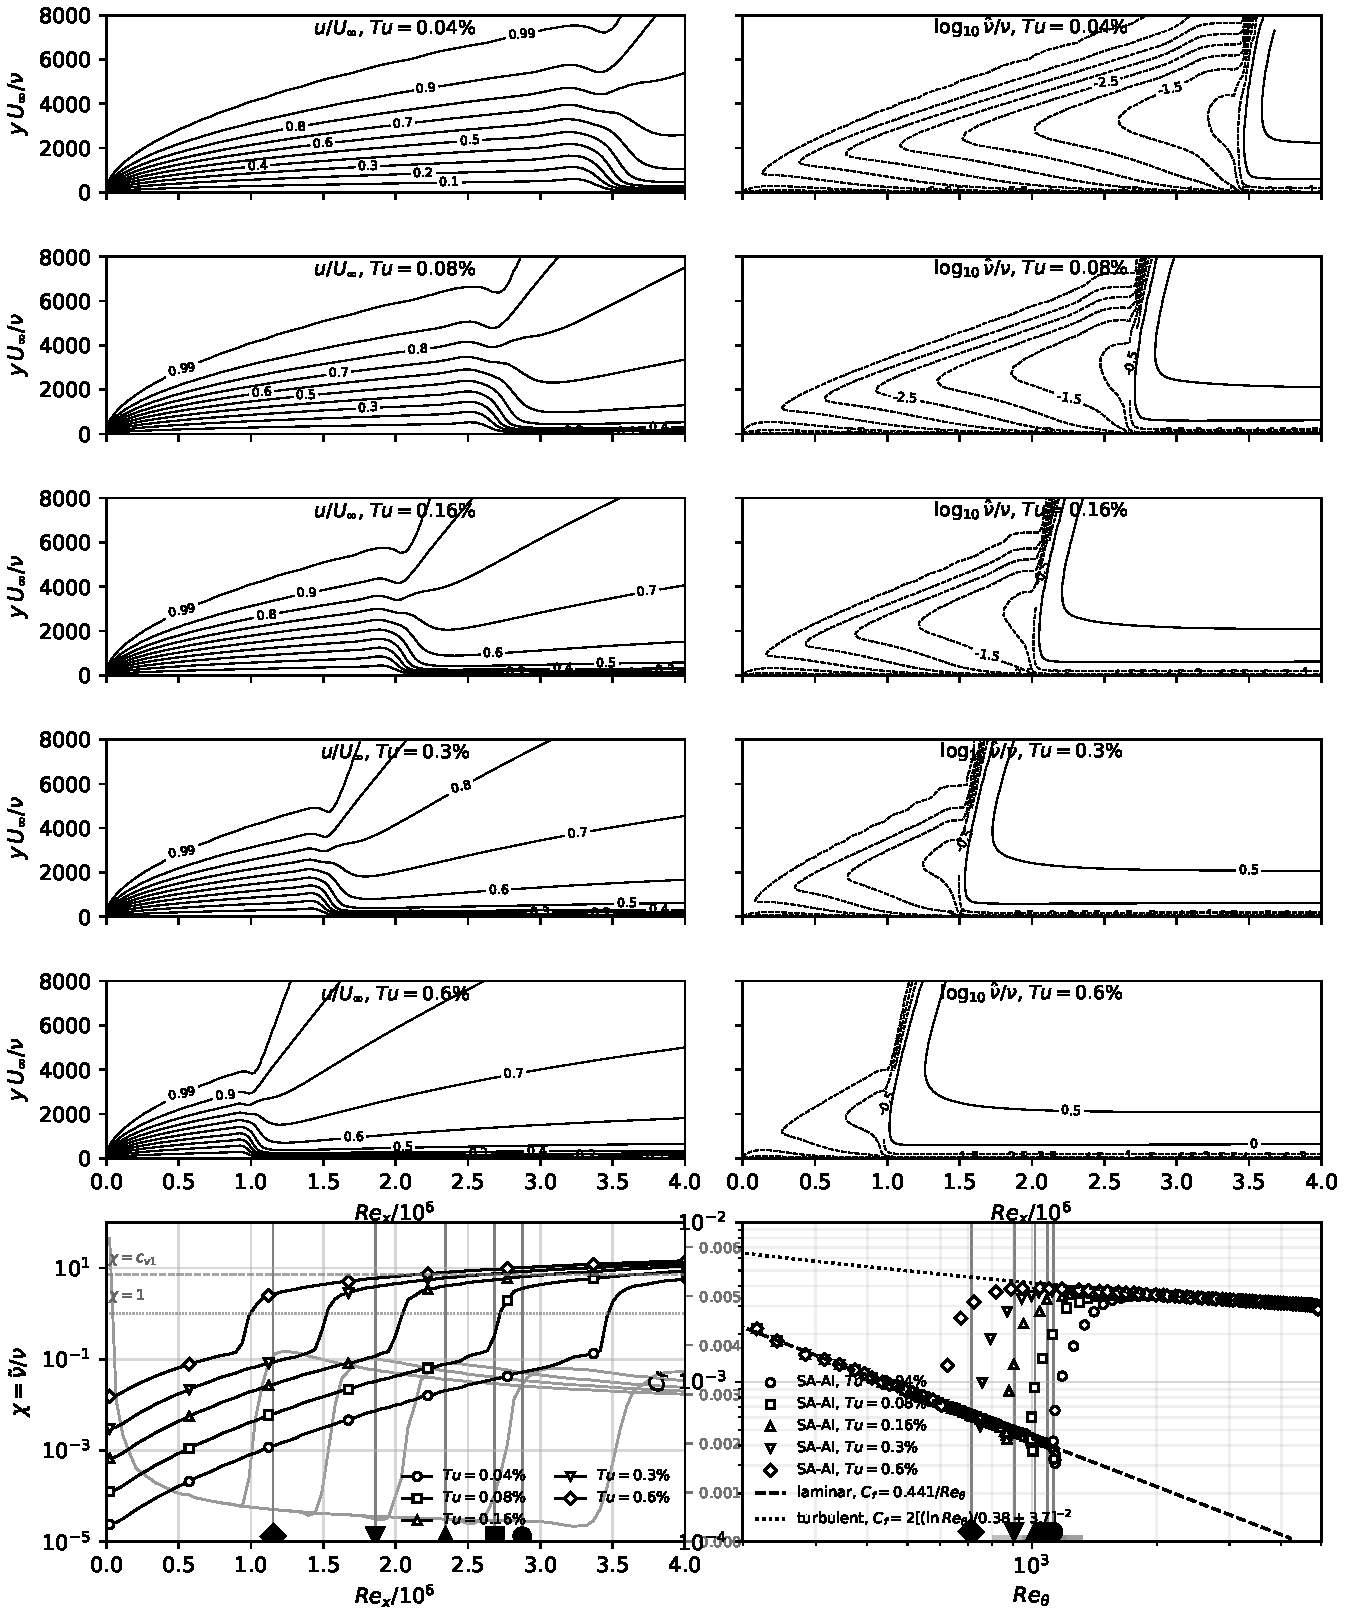
\includegraphics[width=0.90\textwidth]{flat_plate_batch_flow360.pdf}
  \caption{Freestream-turbulence sweep on the flat plate at five levels in the
  natural-transition range $Tu\!=\!0.04$--$0.60\%$ (rows). \emph{Left columns}:
  contours of $u/U_\infty$ and $\log_{10}\hat\nu$ in the $(Re_x,Re_y)$ plane
  ($Re_x\!=\!x\!\cdot\!10^6$). \emph{Bottom-left}: in-BL maximum
  $\chi\!=\!\tilde\nu/\nu$ vs $Re_x$, with horizontal references at $\chi\!=\!1$
  (onset of the $\sigma_t$ blend) and $\chi\!=\!c_{v1}\!=\!7.1$ (eddy-viscosity
  half-saturation). \emph{Bottom-right}: $C_f$ vs $Re_\theta$ with the laminar
  ($C_f\!=\!0.441/Re_\theta$, dashed) and turbulent
  ($C_f\!=\!2[(\ln Re_\theta)/0.38+3.7]^{-2}$, dotted) correlations. Both
  bottom panels use black curves with one symbol per $Tu$ (legend); solid-gray
  verticals and filled bottom-edge symbols mark the Abu-Ghannam \&
  Shaw~\cite{abu_ghannam_shaw_1980} transition-onset reference, and the
  bottom-right adds the digitized Schubauer--Skramstad
  Fig.~7 band (faint bars) for context. With the receptivity taken from Mack's
  $e^N$ correlation, the model's $\chi\!=\!1$ onset tracks
  AGS to within $\sim\!10\%$ across the range and lies within the S-S band; the
  $C_f$ follows the laminar branch then recovers the turbulent correlation,
  a behavior baseline SA cannot produce.}
  \label{fig:flatplate_batch}
\end{figure}

\section{The NLF(1)-0416 airfoil at $Re\!=\!4\!\times\!10^6$}\label{sec:nlfval}

The natural-laminar-flow airfoil NLF(1)-0416 demands an $e^N$-style instability
tracker to be predicted correctly. Its extended favorable-gradient rooftop
sustains a laminar run over nearly half the chord at the design incidence, and
across a wide $\alpha$ range the transition on one surface or the other is
governed by slow Tollmien--Schlichting accumulation rather than a severe adverse
gradient. The model is evaluated at $Re\!=\!4\!\times\!10^6$, $M\!=\!0.1$,
$\chi_\infty\!=\!c_{v1}\,e^{-9}\!\approx\!8.76\!\times\!10^{-4}$
(the $N_\mathrm{crit}\!=\!9$ anchor of Sec.~\ref{sec:calib_tu}; via Mack's
map, Eq.~\eqref{eq:tumap}, it corresponds to $Tu\!\approx\!0.07\%$, consistent
with the low-turbulence tunnel), across
$\alpha\!\in\!\{0^\circ, 4^\circ, 9^\circ,
15^\circ\}$, on a three-level isotropic refinement ladder of both mesh families
(unstructured cavity-mesher and structured O-grid, L0--L2, twenty-four
cases total). The unstructured mesher uses a shared NLF spline contour with
blunt-trailing-edge--aware spacing ($h_\mathrm{TE}$ scales with first-cell
height $h_0$ at every level; the TE ramp ratio $r_\mathrm{TE}$ decays from
$2.0$ at L0 to $1.25$ at L2 so that the local cell size at fixed chord-distance
from the TE also halves); the structured O-grid is generated with the same
contour by Construct2D. Every length scale---surface point count, $h_0$,
growth-ratio offset $(g-1)$, TE step, and TE ramp---refines by a factor of two
per level.
Figures~\ref{fig:nlfmesh_str} and~\ref{fig:nlfmesh_cav} show the two mesh
families at the leading and trailing edges across the three refinement levels,
and Table~\ref{tab:nlfmesh} lists their resolution quantitatively.

\begin{table}[tp]
  \centering
  \small
  \caption{NLF(1)-0416 mesh ladder: size, wall-tangential and wall-normal
  resolution, and resulting $y^+$. Tangential spacing $\Delta s/c$ is measured on
  the upper surface; the wall-normal first-cell height $h_0$ and the cell size
  $0.5c$ off the wall are read from the centre-span slice; the $y^+$ percentiles
  aggregate the four incidences ($\alpha\!=\!0^\circ,4^\circ,9^\circ,15^\circ$).
  The cavity meshes are all-triangular, the structured O-grids all-quadrilateral.}
  \label{tab:nlfmesh}
  \begin{tabular}{l cccccc}
    \toprule
    & \multicolumn{3}{c}{Unstructured cavity} & \multicolumn{3}{c}{Structured O-grid}\\
    \cmidrule(lr){2-4}\cmidrule(lr){5-7}
    & L0 & L1 & L2 & L0 & L1 & L2 \\
    \midrule
    Nodes    & 15{,}268 & 53{,}182 & 193{,}476 & 15{,}920 & 63{,}840 & 255{,}680 \\
    Elements & 29{,}855 & 105{,}481 & 385{,}665 & 15{,}721 & 63{,}441 & 254{,}881 \\
    \addlinespace
    $\Delta s/c$ @ LE ($\times10^{-3}$)      & 0.55 & 0.28 & 0.14 & 5.31 & 2.66 & 1.33 \\
    \quad @ $0.05c$                          & 5.73 & 2.85 & 1.42 & 10.5 & 5.23 & 2.61 \\
    \quad @ $0.25c$                          & 11.3 & 5.59 & 2.78 & 17.6 & 8.81 & 4.40 \\
    \quad @ $0.98c$                          & 6.57 & 6.22 & 4.10 & 2.74 & 1.38 & 0.69 \\
    \quad @ TE                               & 2.70 & 1.75 & 0.98 & 0.72 & 0.38 & 0.20 \\
    \addlinespace
    $h_0/c$ ($\times10^{-6}$)                & 12.6 & 5.6 & 2.6 & 7.0 & 3.5 & 1.8 \\
    cell @ $0.001c$ ($\times10^{-6}c$)       & 227 & 97 & 49 & 159 & 82 & 43 \\
    cell @ $0.5c$ ($\times10^{-2}c$)         & 8.45 & 4.41 & 2.21 & 2.19 & 1.07 & 0.52 \\
    \addlinespace
    $y^+$ (95th pct)                         & 2.99 & 2.10 & 1.22 & 1.90 & 0.92 & 0.46 \\
    $y^+$ (99th pct)                         & 4.26 & 3.12 & 2.05 & 2.53 & 1.39 & 0.70 \\
    \bottomrule
  \end{tabular}
\end{table}

The unstructured family is deliberately adversarial. Unlike the usual
``unstructured'' airfoil mesh---which grows a \emph{structured} layer of
wall-normal quadrilaterals or prisms through the boundary layer and triangulates
only the isotropic exterior---the cavity mesher applies the same
constrained-Delaunay triangulation everywhere, the boundary layer
included. There the metric is stretched by
$O(10^2\text{--}10^3)\!:\!1$, and the cavity point-insertion uses an anisotropic
distortion metric (with a skewness/normal-deviation objective) to promote
near-right-angled stretched triangles ($\sim\!90^\circ$-$90^\circ$-$0^\circ$)
over flat slivers ($\sim\!180^\circ$-$0^\circ$-$0^\circ$); but this is a
preference, not a guarantee, and the resolved boundary layer carries many
near-degenerate triangles (visible in Fig.~\ref{fig:nlfmesh_cav}, and reflected in
the elevated peak $y^+$ of the cavity grids in Table~\ref{tab:nlfmesh}). This directly
stresses the model, whose indicators ($Re_\Omega$, $\Gamma$, $\lambda_p$) are
all \emph{local} and gradient-based,
so sliver-induced errors in the least-squares gradients feed
straight into the amplification rate. That the cavity and O-grid families
nevertheless predict the same transition---agreeing in drag to within
$\Delta C_d\!\approx\!6\!\times\!10^{-4}$ through $\alpha\!=\!4^\circ$ (rising to
$\approx\!1$--$1.6\!\times\!10^{-3}$ at $\alpha\!=\!9^\circ$--$15^\circ$, the
$9^\circ$ gap set by the marginal cavity near-LE onset) at L2---is therefore a
genuine robustness result, not merely a grid-convergence check.

\begin{figure}[tp]
  \centering
  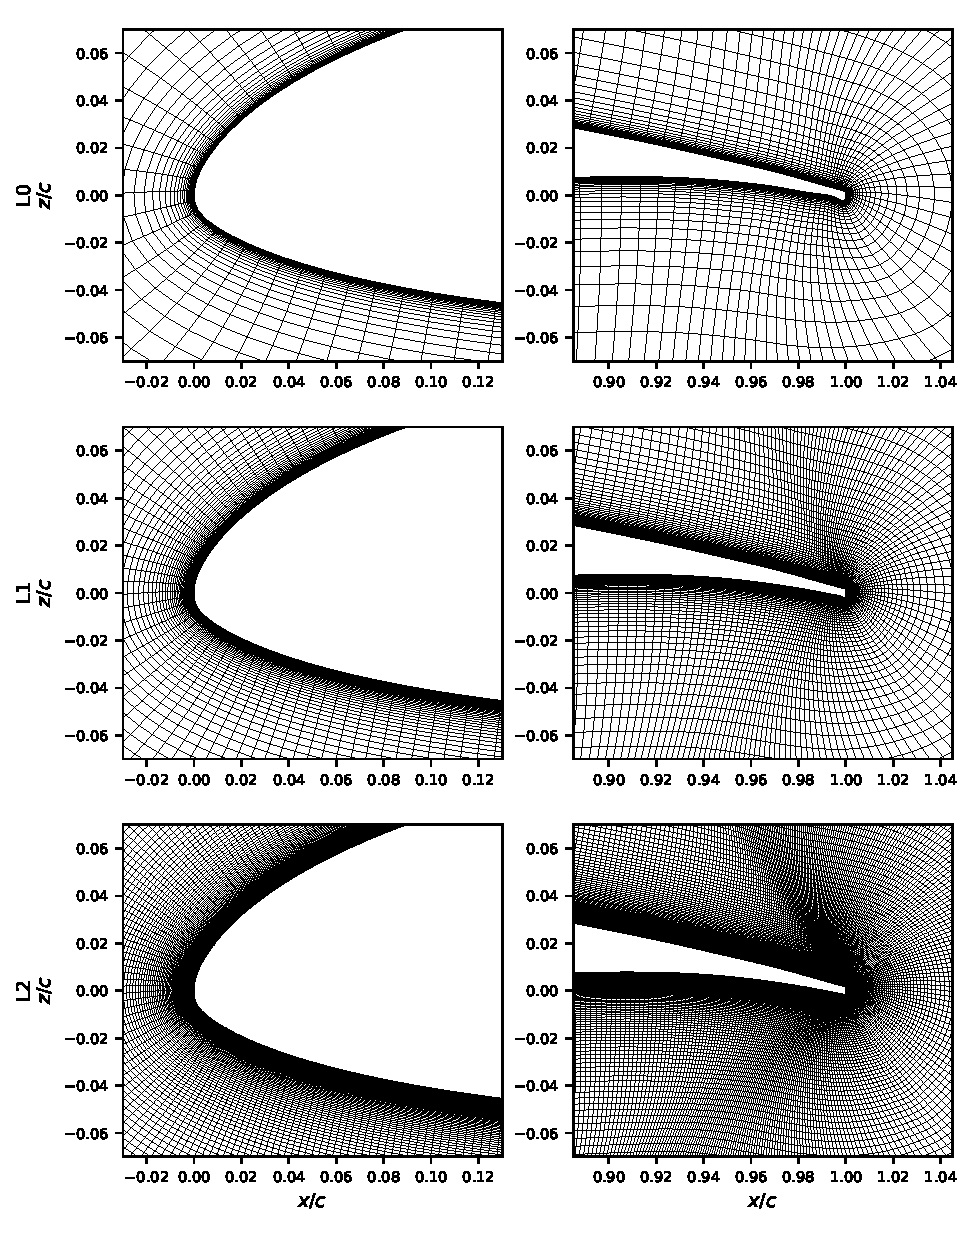
\includegraphics[width=0.9\textwidth]{mesh_nlf_str.pdf}
  \caption{NLF(1)-0416 structured O-grid mesh at the leading edge (left column)
  and blunt trailing edge (right column) for the three refinement levels
  L0--L2 (rows). The O-grid wraps the section with wall-normal clustering for
  the boundary layer; every length scale halves per level. Chord normalized to
  unity ($z$ vertical).}
  \label{fig:nlfmesh_str}
\end{figure}

\begin{figure}[tp]
  \centering
  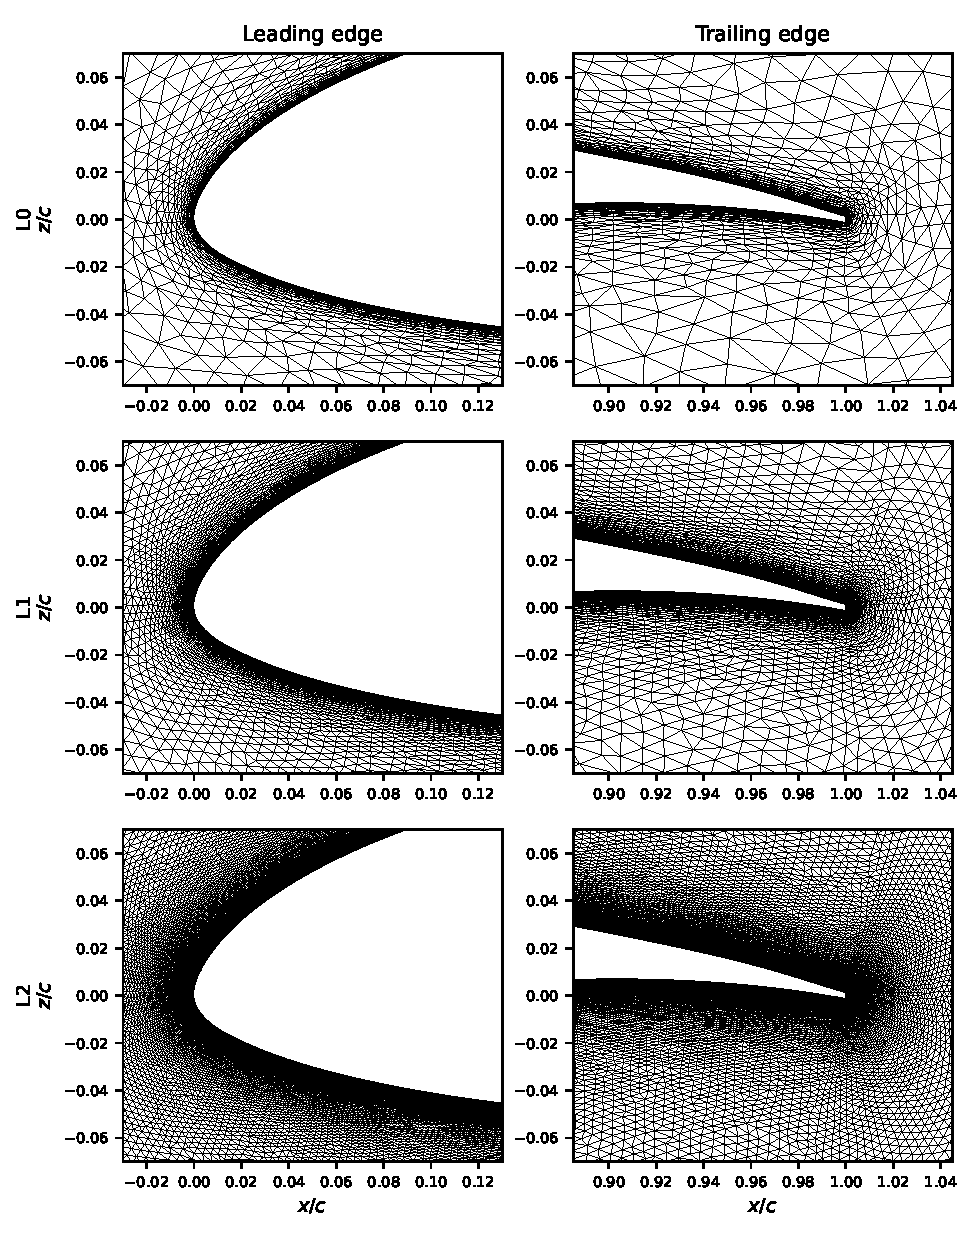
\includegraphics[width=0.9\textwidth]{mesh_nlf_cav.pdf}
  \caption{NLF(1)-0416 unstructured cavity mesh (leading and trailing edges,
  levels L0--L2), built from the same spline contour as the structured grid of
  Fig.~\ref{fig:nlfmesh_str} with blunt-trailing-edge--aware spacing. Every
  length scale halves per level.}
  \label{fig:nlfmesh_cav}
\end{figure}

The airfoil surface distributions are presented as five-row figures
(Figs.~\ref{fig:nlfcflow}--\ref{fig:nlfcfhigh} here and
Figs.~\ref{fig:eppcflow}--\ref{fig:eppcfhigh} for the Eppler 387) with a
common layout: \emph{row 1} the wall-normal-probe maximum of $Re_\Omega$
(log); \emph{row 2} the pressure-gradient/profile indicator governing
that section, evaluated over the kernel-active band ($Re_\Omega\!>\!\tfrac12
\max_y Re_\Omega$, the $\theta$-scale layer around the $Re_\Omega$ peak): for the
NLF (favorable-PG regime) this is the streamwise pressure-gradient parameter
$\lambda_p$ of Eq.~\eqref{eq:indicators} (reference line at $\lambda_p\!=\!0$,
separating favorable $\lambda_p\!>\!0$ where the cliff delays onset from adverse
$\lambda_p\!<\!0$); \emph{row 3} the in-BL maximum
$\chi\!=\!\max_y\tilde\nu/\nu$ on a log axis with the amplification factor $N$ from
mfoil~\cite{fidkowski_mfoil_2022}, a coupled viscous--inviscid $e^N$ panel solver,
on a linear right axis, the two linked by $N\!=\!\ln(\chi/\chi_\infty)$ so
one unit on the right equals one $e$-fold on the left (vertical dotted lines:
mfoil $x_\mathrm{tr}$); \emph{row 4} $-C_p$; \emph{row 5} $C_f$---signed for
the Eppler 387, whose bubble carries reversed near-wall flow
(Sec.~\ref{sec:eppval}), unsigned for the NLF, whose boundary layers stay
attached.
Throughout, color encodes the surface (upper blue, lower red), line style the
mesh family (structured O-grid solid, unstructured cavity dashed), and line
thickness the refinement level (L0 thinnest, L2 thickest); dotted curves are
the mfoil $e^9$ reference. Surfaces are separated by walking the airfoil
contour through the mesh connectivity and splitting at the geometric LE/TE
extrema rather than by the sign of $z$, which is essential on the NLF because
the reflex camber places the lower surface above the chord line over the aft
region.

\begin{figure}[tp]
  \centering
  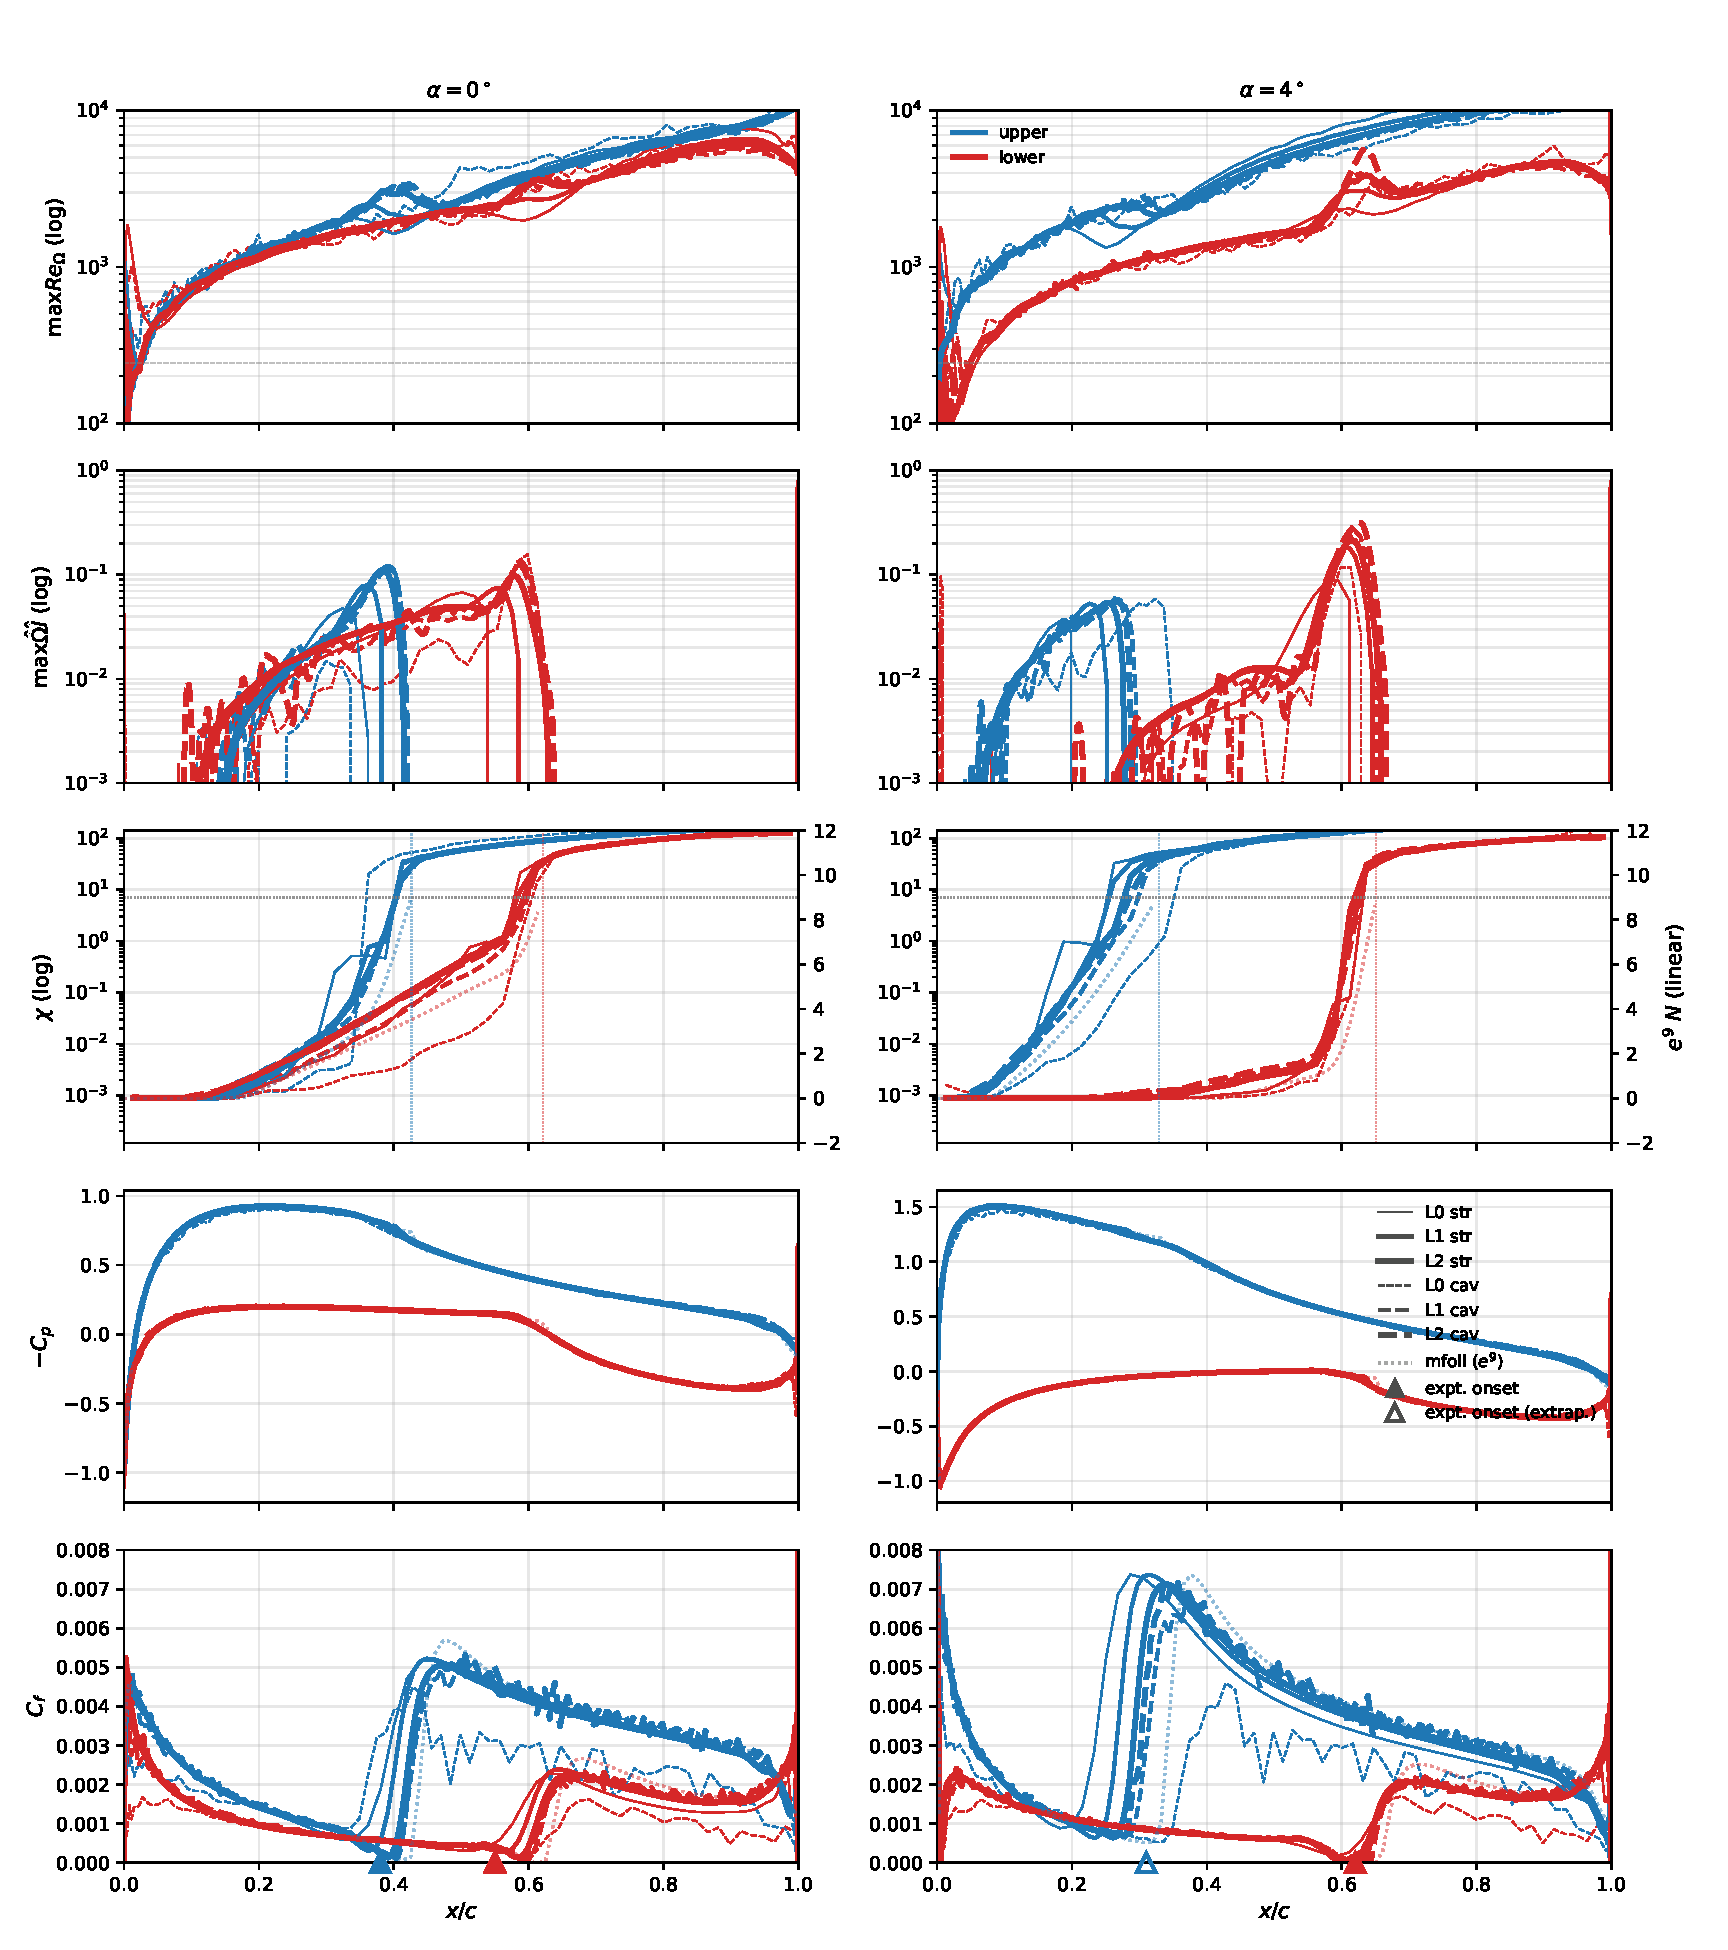
\includegraphics[width=0.86\textwidth]{nlf_cf_lowalpha.pdf}
  \caption{NLF(1)-0416 surface distributions at $\alpha\!\in\!\{0^\circ,4^\circ\}$,
  $Re\!=\!4\!\times\!10^6$, $\chi_\infty\!=\!8.76\!\times\!10^{-4}$. Five-row
  layout and line conventions as described in the text (row~1 $\max Re_\Omega$,
  row~2 $\lambda_p$, row~3 $\chi$ with mfoil $N$, row~4 $-C_p$,
  row~5 $C_f$; upper blue / lower red, O-grid solid / cavity dashed,
  L0--L2 by thickness, mfoil $e^9$ dotted). At $\alpha\!=\!0^\circ$ both
  surfaces transition near $x/c\!\approx\!0.45$, recovering the low-drag
  bucket; at $\alpha\!=\!4^\circ$ the upper-surface transition has marched
  forward to $x/c\!\approx\!0.30$ while the lower stays near design. The
  transition locations track the $e^9$ envelope to within $\sim\!0.06\,c$ and
  the measured onsets (Table~\ref{tab:nlftrans}) to within $\sim\!0.05\,c$
  on both surfaces, both meshes, and at every refinement level from L0
  ($N{\approx}200$ surface points) to L2 ($N{=}800$).}
  \label{fig:nlfcflow}
\end{figure}

\begin{figure}[tp]
  \centering
  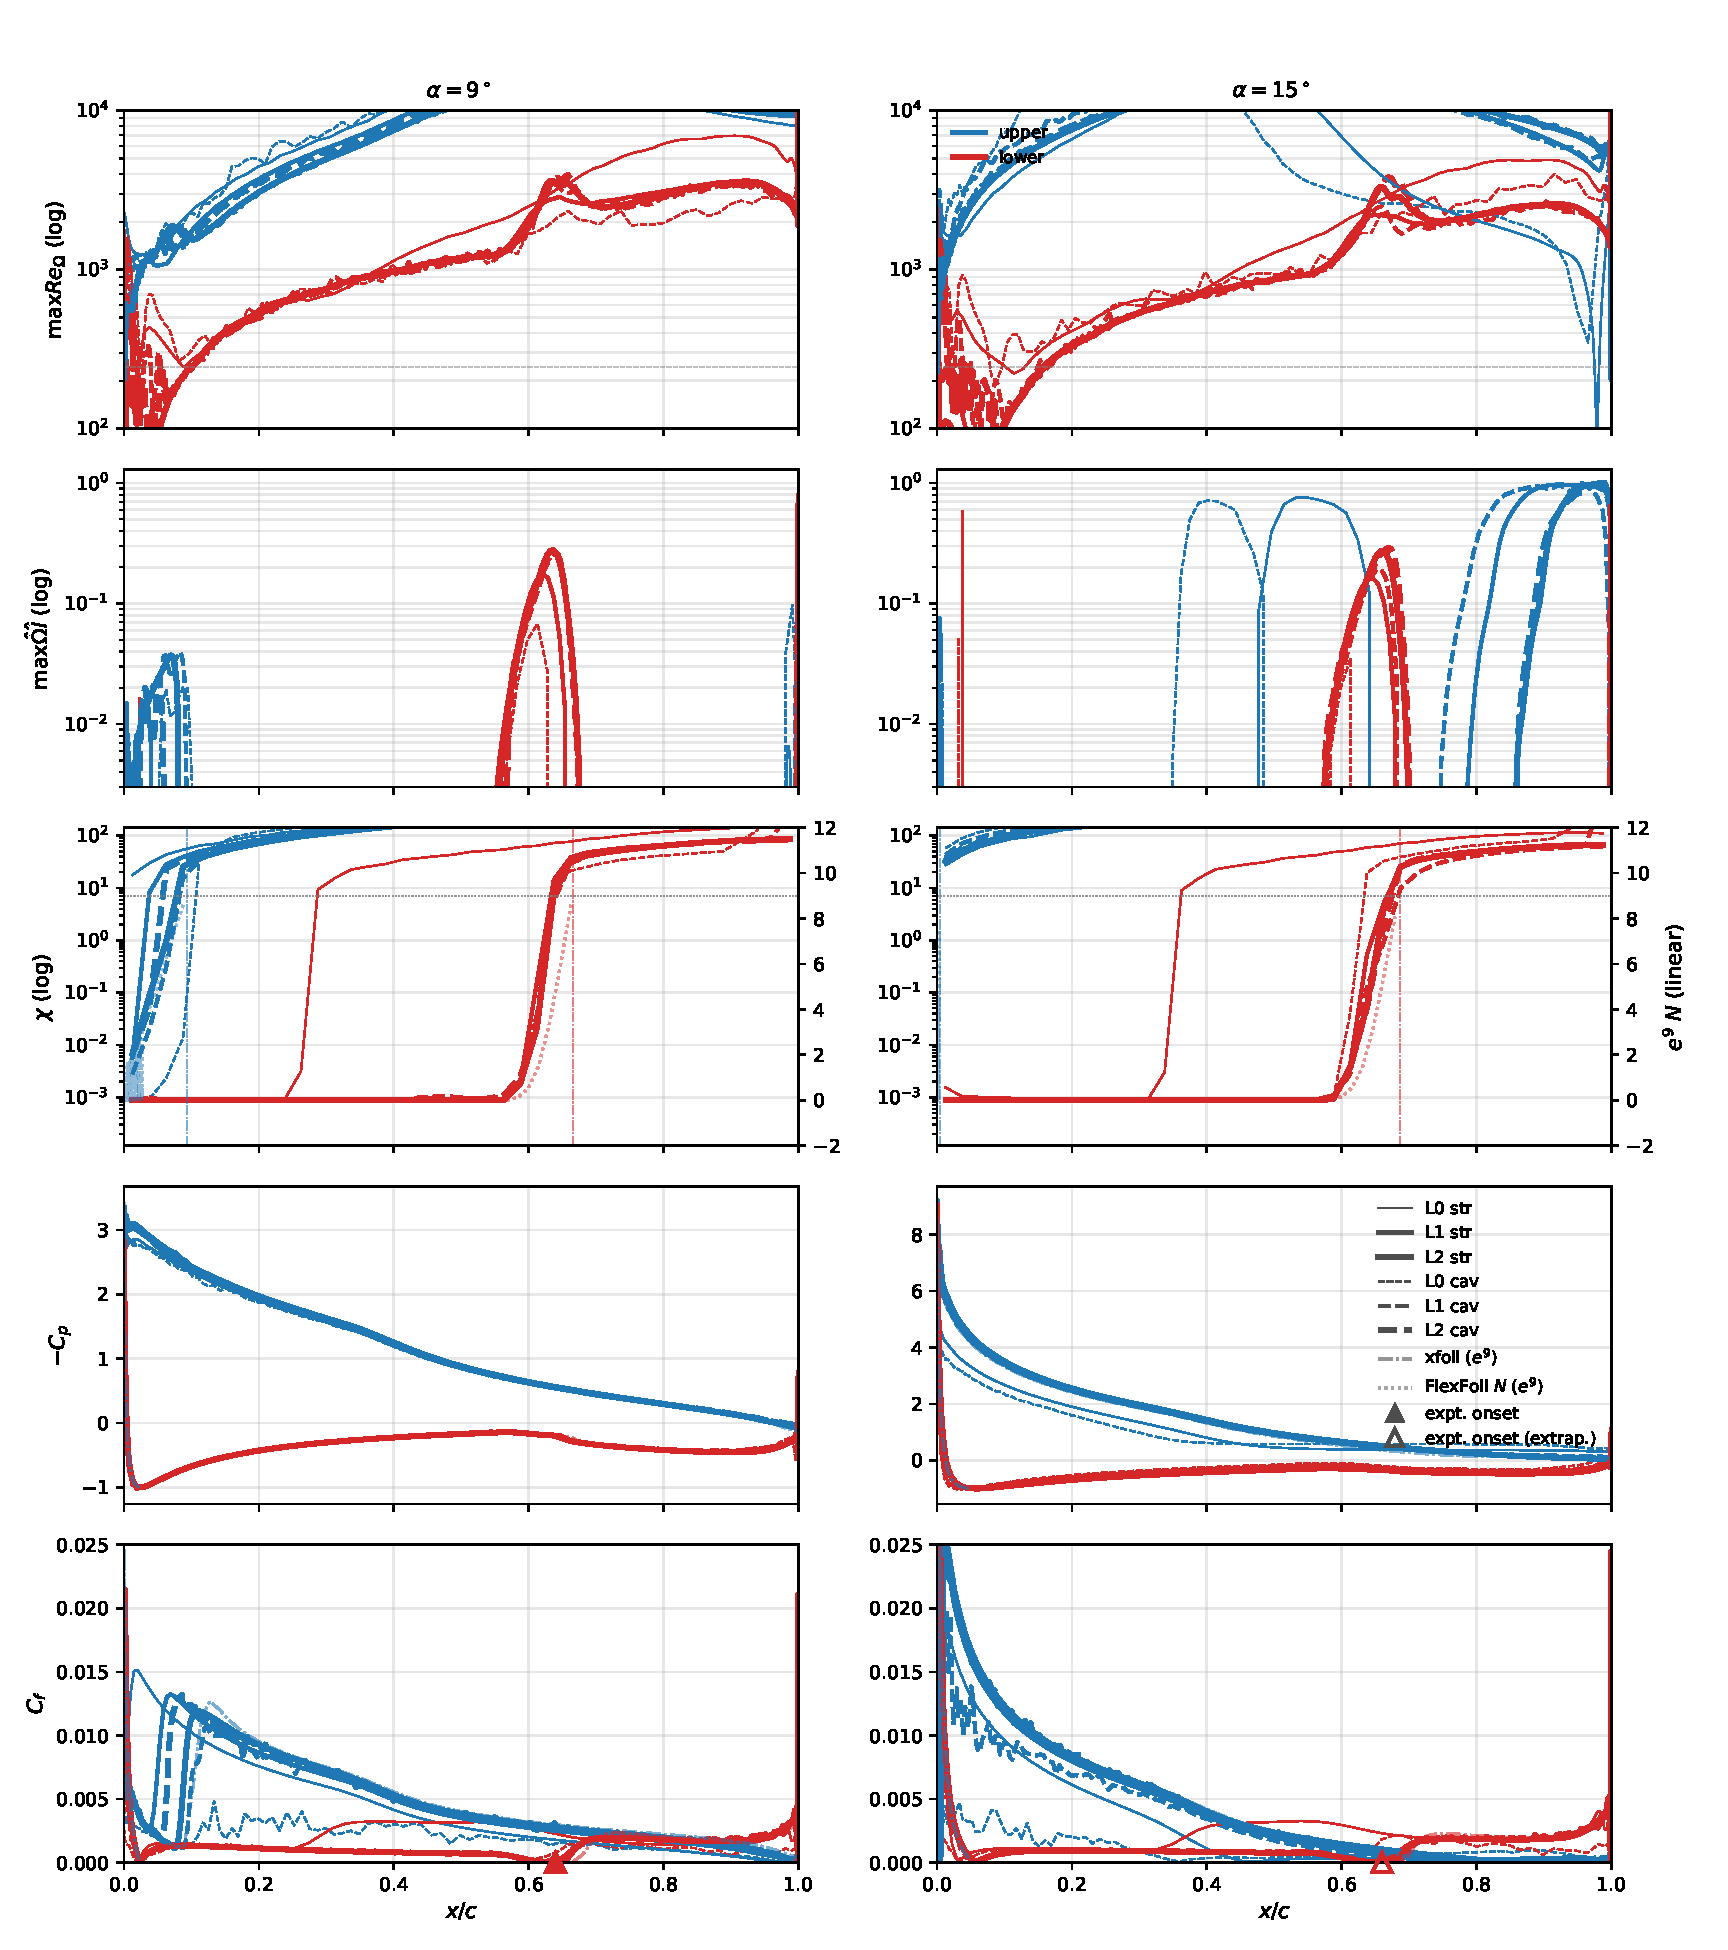
\includegraphics[width=0.86\textwidth]{nlf_cf_highalpha.pdf}
  \caption{As Fig.~\ref{fig:nlfcflow}, at $\alpha\!\in\!\{9^\circ,15^\circ\}$.
  The upper-surface transition has marched to $x/c\!\lesssim\!0.05$ at
  $\alpha\!=\!9^\circ$ and is at the LE by $\alpha\!=\!15^\circ$, while the
  lower transition remains aft of mid-chord. mfoil does not converge at
  $\alpha\!=\!9^\circ$ and stalls at $15^\circ$, so the $e^9$ overlay here is
  XFOIL's~\cite{drela_xfoil_1989} (dash-dot: $C_p$, $C_f$, and transition
  location); the continuous amplification envelope $N(x)$
  is a mfoil output and so is absent at these incidences (row~3 shows only the
  transition marker). The L0 unstructured under-resolves
  the LE suction peak by $\sim\!1$ in $-C_p$ at $\alpha\!=\!15^\circ$ (thin
  dashed blue); L1/L2 collapse on both grids. The high-incidence cases are an
  unforgiving test of the amplification model under a strong adverse gradient:
  $\chi$ rises through $c_{v1}$ within the first few percent of chord on the
  upper surface, but the model still resolves a finite laminar dip and the
  laminar/turbulent handover stays at one chordwise location across the
  refinement series.}
  \label{fig:nlfcfhigh}
\end{figure}

The skin friction (Figs.~\ref{fig:nlfcflow}--\ref{fig:nlfcfhigh}, bottom rows)
follows the laminar branch upstream of the transition front and recovers a
turbulent level downstream at every operating point; both
surfaces and both mesh families place the rise at the same chordwise location at
L1 and L2. The
pressure distributions (middle rows)
are essentially identical between L1 and L2 on each grid, including the strong
leading-edge suction at $\alpha\!=\!15^\circ$ where $-C_{p,\max}\!\approx\!8$:
the only visible refinement effect is L0 unstructured under-predicting the LE
peak by $\sim\!1$ in $-C_p$ at $\alpha\!=\!15^\circ$ (a leading-edge
$y^+$/resolution effect that the L1 mesh removes).

Table~\ref{tab:nlftrans} places the computed onset locations against the
wind-tunnel
measurements of Somers~\cite{somers_1981}, whose surface transition orifices
(open where the flow is laminar, solid where turbulent) locate the front on each
surface as a function of $c_l$; we read that curve at the computed section
$c_l$. On the lower surface, where the experiment resolves the front across the
whole $c_l$ range, SA-AI matches the measured $x_\mathrm{tr}$ to within
$\sim\!0.03\,c$ at every incidence, reproducing the mild aft-ward march
($0.53\!\to\!0.64\,c$) as the lift rises; the $e^9$ panel solver sits
$\sim\!0.03$--$0.09\,c$ downstream of both. On the upper surface the model
recovers the measured onset at $\alpha\!=\!0^\circ$
(SA-AI $0.37\,c$, experiment $0.38\,c$) and marches the front forward with
incidence---to $0.25\,c$ at $\alpha\!=\!4^\circ$, against a measured front
extrapolated to $\approx\!0.31\,c$ just ahead of the forwardmost orifice
($x/c\!\approx\!0.30$); at higher incidence the upper onset moves too far forward
for the orifices to locate. The $Re\!=\!2\!\times\!10^6$ oil-flow
photographs (Somers' Fig.~7) independently show the same forward march, from a
laminar-separation bubble near mid-chord at $\alpha\!=\!0^\circ$ ($c_l\!=\!0.4$)
to roughly a third-chord by $\alpha\!=\!8^\circ$ ($c_l\!=\!1.3$). mfoil fails to
converge at $\alpha\!=\!9^\circ$ and
stalls at $15^\circ$; XFOIL~\cite{drela_xfoil_1989}, the reference $e^9$ solver,
supplies the $e^9$ comparison there
(Table~\ref{tab:nlftrans}), agreeing with the present RANS
to within $\sim\!0.03\,c$ in transition location.

\begin{table}[tp]
  \centering
  \small
  \caption{Transition location $x_\mathrm{tr}/c$ on the NLF(1)-0416 at
  $Re\!=\!4\!\times\!10^6$, by surface and incidence. \emph{SA-AI}: present
  model on the finest structured O-grid (L2), with onset defined as the first
  station where the near-wall maximum $\chi$ crosses unity (the start of the
  $\sigma_t$ blend, Sec.~\ref{sec:flatplate}); the cavity
  L2 grid agrees to within $0.01\,c$ except at the $\alpha\!=\!9^\circ$ upper
  (marginal near-LE onset, $0.03\,c$) and the slowly-settling
  $\alpha\!=\!0^\circ$ lower front ($0.03\,c$). \emph{$e^9$}: coupled viscous--inviscid
  panel solvers---mfoil~\cite{fidkowski_mfoil_2022}, or
  XFOIL~\cite{drela_xfoil_1989} where marked~$^\dagger$. \emph{Exp}: Somers
  (NASA TP-1861, Fig.~9d), transition orifices (open laminar / solid turbulent)
  read as $x_\mathrm{tr}(c_l)$ and mapped through the computed section $c_l$; the
  upper onset at $\alpha\!\geq\!9^\circ$ marches too far forward for the orifices
  to locate (---). $^\ddagger$Extrapolated beyond the recorded orifices: the
  upper front at $\alpha\!=\!4^\circ$ (just ahead of the forwardmost orifice,
  $x/c\!\approx\!0.30$) and the lower front at $\alpha\!=\!15^\circ$ (along the
  nearly flat lower branch, beyond the measured $c_{l,\max}\!\approx\!1.68$).
  $^\dagger$From XFOIL: mfoil fails at these incidences.}
  \label{tab:nlftrans}
  \begin{tabular}{cc ccc c ccc}
    \toprule
    & & \multicolumn{3}{c}{Upper $x_\mathrm{tr}/c$} & & \multicolumn{3}{c}{Lower $x_\mathrm{tr}/c$}\\
    \cmidrule(lr){3-5}\cmidrule(lr){7-9}
    $\alpha$ & $c_l$ & SA-AI & $e^9$ & Exp & & SA-AI & $e^9$ & Exp \\
    \midrule
    $0^\circ$  & 0.49 & 0.37 & 0.43 & 0.38 & & 0.53 & 0.62 & 0.55 \\
    $4^\circ$  & 0.96 & 0.25 & 0.33 & $0.31^\ddagger$ & & 0.60 & 0.65 & 0.62 \\
    $9^\circ$  & 1.48 & 0.08 & $0.09^\dagger$ & ---  & & 0.61 & $0.67^\dagger$ & 0.64 \\
    $15^\circ$ & 1.95 & 0.00 & $0.00^\dagger$ & ---  & & 0.64 & $0.69^\dagger$ & $0.66^\ddagger$ \\
    \bottomrule
  \end{tabular}
\end{table}

\subsection{Marginal natural transition and the production blend}\label{sec:blendnlf}

The form of the production blend~\eqref{eq:blend}---a $\max$ rather than a convex
combination---matters on the NLF(1)-0416. Its long favorable-gradient rooftop
keeps the boundary layer near neutral over an extended chord, so transition is
marginal and the early-turbulent region just past $\chi\!=\!1$ sits close behind
the front. A convex blend $\sigma_P P_\mathrm{SA}+(1-\sigma_P)P_\mathrm{AI}$
would leave a $(1-\sigma_P)P_\mathrm{AI}$ bleed there, keeping the
\emph{pressure-sensitive} amplification weighted into that region and coupling the
front---through the airfoil's circulation---to the outer pressure field. The
$\max$ form removes it: once $\sigma_P P_\mathrm{SA}$ overtakes amplification just
past $\chi\!=\!1$ the production is the pressure-\emph{insensitive} SA term, so the
front carries no residual receptivity to the outer pressure field, while the
laminar amplification is untouched ($\max$ and convex coincide for
$\chi\!\le\!1$).

A grid artifact on the coarsest structured mesh exposes the streamwise-resolution
demand transition places on the model. On L0 the
amplification factor $\chi\!=\!\max_y\tilde\nu/\nu$
stalls and dips over the two cells preceding transition (at $\alpha\!=\!4^\circ$
from $0.82$ to $0.60$; at $\alpha\!=\!0^\circ$ from $0.41$ to $0.31$) before jumping
one-to-two orders of magnitude to its turbulent level across a single cell. The
cause is not the $\sigma_t$ handover---there $\chi\!<\!1$, so $\sigma_t\!=\!0$ and
the eddy viscosity is still negligible. It is the under-resolved jump reaching
upstream: spread over less than one cell, the abrupt laminar-to-turbulent change in
profile shape generates a discretization error that propagates two to three cells
upstream and subtly distorts the velocity profile. The profile-fullness indicator
$\Gamma$ at the amplifying ($\tilde\nu$-peak) point reads this distortion and
collapses from $\approx\!1.1$ to $\approx\!0.5$; because the rate is gated by the
$\Gamma$-sigmoid centered at $g_c\!=\!1.572$, the amplification rate falls
twentyfold ($a\!\approx\!0.010\!\to\!0.0005$), switching growth off. The effect is
purely numerical---on L1 and L2 the same $\Gamma$ holds near $1.1$ through the
identical station and $\chi$ rises monotonically---and its only trace in the
solution is a small shift in the resolved onset that converges out by L1.

\begin{figure}[tp]
  \centering
  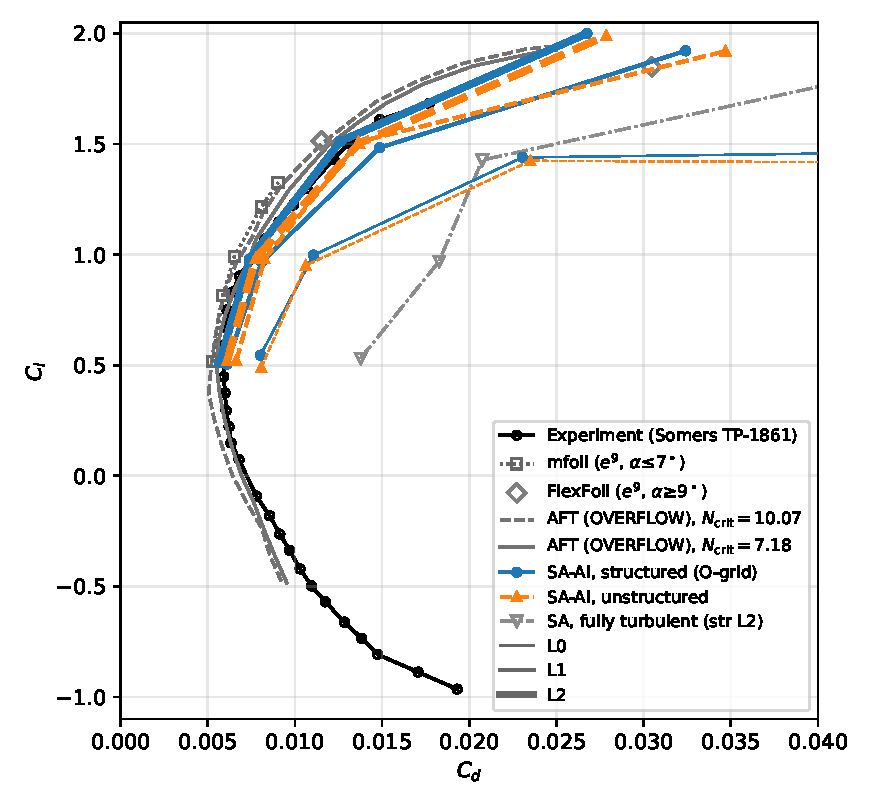
\includegraphics[width=0.62\textwidth]{nlf_polar_compare.pdf}
  \caption{Drag polar of the NLF(1)-0416 at $Re\!=\!4\!\times\!10^6$: the present
  SA-AI prediction (structured O-grid and unstructured meshes, all three
  refinement levels) at $\alpha\!\in\!\{0^\circ,4^\circ,9^\circ,15^\circ\}$
  overlaid on the digitized experimental section characteristics (Somers, NASA
  TP-1861, Fig.~11d~\cite{somers_1981}) and the mfoil $e^9$ reference. Mesh family
  sets the colour (blue = O-grid, orange = unstructured); refinement sets the line
  weight (L0 thin $\to$ L2 thick). The mfoil reference (grey squares) is shown
  where its coupled solve converges to an attached solution ($\alpha\!\le\!7^\circ$);
  at $\alpha\!=\!9^\circ$ and $15^\circ$, where mfoil fails, the $e^9$ reference is
  XFOIL's (grey diamonds), which converges there. The grey dash-dot curve is
  fully turbulent SA ($\chi_\infty\!=\!3$, same solver, structured L2 grid):
  without the laminar run the drag sits $57$--$76\%$ above the bucket.}
  \label{fig:nlfpolar}
\end{figure}

The section drag summarizes the transition prediction
(Fig.~\ref{fig:nlfpolar}). On the refined meshes the SA-AI polar tracks the
measured low-drag laminar bucket across $\alpha\!\in\!\{0^\circ,4^\circ,9^\circ\}$,
with the computed $C_d$ within $\sim\!5\times10^{-4}$ of the digitized data
through the bucket and up the upper knee.
The $\alpha\!=\!15^\circ$ point lies beyond the measured stall
($C_{l,\max}\!\approx\!1.68$ in the tunnel data), where the quasi-2D computation
does not capture three-dimensional stall and returns a higher $C_l$ at elevated
drag. The coarse L0 mesh over-predicts drag at $\alpha\!\ge\!9^\circ$
(under-resolved transition front). The mfoil $e^9$ reference follows the same
bucket through $\alpha\!=\!7^\circ$ ($C_l\!=\!1.33$) but provides no valid point
at higher incidence; since XFOIL converges at the identical conditions
($C_l\!=\!1.52$ at $\alpha\!=\!9^\circ$, consistent with the present RANS), the
fault lies in mfoil's Newton globalization, not the method
class. A fully turbulent SA computation on the same structured L2 grid (grey
dash-dot in Fig.~\ref{fig:nlfpolar}) quantifies what the transition model
recovers: with the boundary layers effectively tripped from the leading edge,
its drag is $C_d\!=\!0.0099$--$0.0113$ at the bucket incidences
($\alpha\!=\!0^\circ,4^\circ$), $57$--$76\%$ above the SA-AI laminar-flow
level, and closes on the SA-AI polar only as the laminar run shrinks at high
incidence ($+29\%$ at $9^\circ$, $+10\%$ at $15^\circ$).

\section{The Eppler 387 low-Reynolds-number airfoil}\label{sec:eppval}

The Eppler 387 closes the study with the
adverse-pressure-gradient regime. The McGhee, Walker, and Millard experiment in
the NASA Langley Low-Turbulence Pressure Tunnel \cite{mcghee_1988} tested this
airfoil from $Re\!=\!6\!\times\!10^4$ to $4.6\!\times\!10^5$ at tunnel
turbulence levels between $0.06\%$ and $0.18\%$; the data are the canonical
reference for low-$Re$ transition modeling and supply the comparison condition
used by Coder and Maughmer's AFT-2014, Coder's AFT-2017, the Langtry--Menter
$\gamma$--$Re_\theta$ benchmark, and the Bas--{\c C}akmak{\c c}{\i}o{\u g}lu
algebraic SA-BCM variant
\cite{coder_maughmer_2014, halila_2022, langtry_menter_2009, cakmakcioglu_2018}.
At these conditions the upper surface carries a long laminar-separation bubble
(LSB) that controls the section drag: laminar separation at the shoulder of the
suction peak, an inflectional shear layer in which the rate kernel must
accelerate amplification, turbulent reattachment, and a short turbulent wedge
to the trailing edge.

The model is evaluated at the de-facto benchmark condition of the
transition-modeling literature: $Re\!=\!2\!\times\!10^5$, $M\!=\!0.1$, across
$\alpha\!\in\!\{0^\circ,2^\circ,5^\circ,7^\circ\}$, with the freestream seed at
the same $N_\mathrm{crit}\!=\!9$ anchor as the NLF,
$\chi_\infty\!=\!8.76\!\times\!10^{-4}$ (the LTPT-class value). Three
refinement levels on two independently-generated mesh families
(unstructured cavity, structured O-grid) give twenty-four cases.

Mesh generation reuses the NLF recipe verbatim. The 56-point Eppler 387
contour is read from the NASA TM 4062 Table I (design coordinates with the
trailing edge thickened from $0$ to $0.01\,\mathrm{in}$ blended at
$x/c\!=\!0.95$; $z_\mathrm{TE}\!=\!\pm0.000833\,c$, half the NLF
blunt-thickness), spline-interpolated, resampled at $N\!\in\!\{200,400,800\}$
points with piecewise-cosine clustering at the LE and TE, and fed to both the
in-house unstructured cavity mesher and Construct2D; the far-field is fixed at
$100\,c$. The resulting grids range
from $1.5\!\times\!10^4$ nodes at L0 to $2.6\!\times\!10^5$ at L2.
Figures~\ref{fig:eppmesh_str} and~\ref{fig:eppmesh_cav} show the two mesh
families at the leading and trailing edges across the three levels, and
Table~\ref{tab:eppmesh} lists their resolution quantitatively.

\begin{table}[tp]
  \centering
  \small
  \caption{Eppler 387 mesh ladder: size, wall-tangential and wall-normal
  resolution, and resulting $y^+$, measured as in Table~\ref{tab:nlfmesh}; the
  $y^+$ percentiles aggregate the four incidences
  ($\alpha\!=\!0^\circ,2^\circ,5^\circ,7^\circ$). The lower Reynolds number
  ($2\times10^5$) keeps $y^+$ well below unity on every grid. The cavity meshes
  are all-triangular, the structured O-grids all-quadrilateral.}
  \label{tab:eppmesh}
  \begin{tabular}{l cccccc}
    \toprule
    & \multicolumn{3}{c}{Unstructured cavity} & \multicolumn{3}{c}{Structured O-grid}\\
    \cmidrule(lr){2-4}\cmidrule(lr){5-7}
    & L0 & L1 & L2 & L0 & L1 & L2 \\
    \midrule
    Nodes    & 15{,}219 & 53{,}109 & 192{,}714 & 15{,}920 & 63{,}840 & 255{,}680 \\
    Elements & 29{,}757 & 105{,}335 & 384{,}141 & 15{,}721 & 63{,}441 & 254{,}881 \\
    \addlinespace
    $\Delta s/c$ @ LE ($\times10^{-3}$)      & 1.13 & 0.57 & 0.28 & 4.94 & 2.48 & 1.24 \\
    \quad @ $0.05c$                          & 5.28 & 2.63 & 1.31 & 9.82 & 4.88 & 2.43 \\
    \quad @ $0.25c$                          & 11.0 & 5.46 & 2.72 & 17.4 & 8.63 & 4.30 \\
    \quad @ $0.98c$                          & 15.1 & 5.04 & 3.32 & 2.68 & 1.32 & 0.69 \\
    \quad @ TE                               & 2.27 & 2.97 & 0.86 & 0.58 & 0.32 & 0.19 \\
    \addlinespace
    $h_0/c$ ($\times10^{-6}$)                & 14.3 & 5.7 & 2.8 & 6.6 & 3.3 & 1.7 \\
    cell @ $0.001c$ ($\times10^{-6}c$)       & 226 & 98 & 51 & 168 & 86 & 44 \\
    cell @ $0.5c$ ($\times10^{-2}c$)         & 8.20 & 4.33 & 2.23 & 1.91 & 0.94 & 0.45 \\
    \addlinespace
    $y^+$ (95th pct)                         & 0.35 & 0.17 & 0.08 & 0.11 & 0.05 & 0.03 \\
    $y^+$ (99th pct)                         & 0.43 & 0.27 & 0.13 & 0.15 & 0.08 & 0.04 \\
    \bottomrule
  \end{tabular}
\end{table}

\begin{figure}[tp]
  \centering
  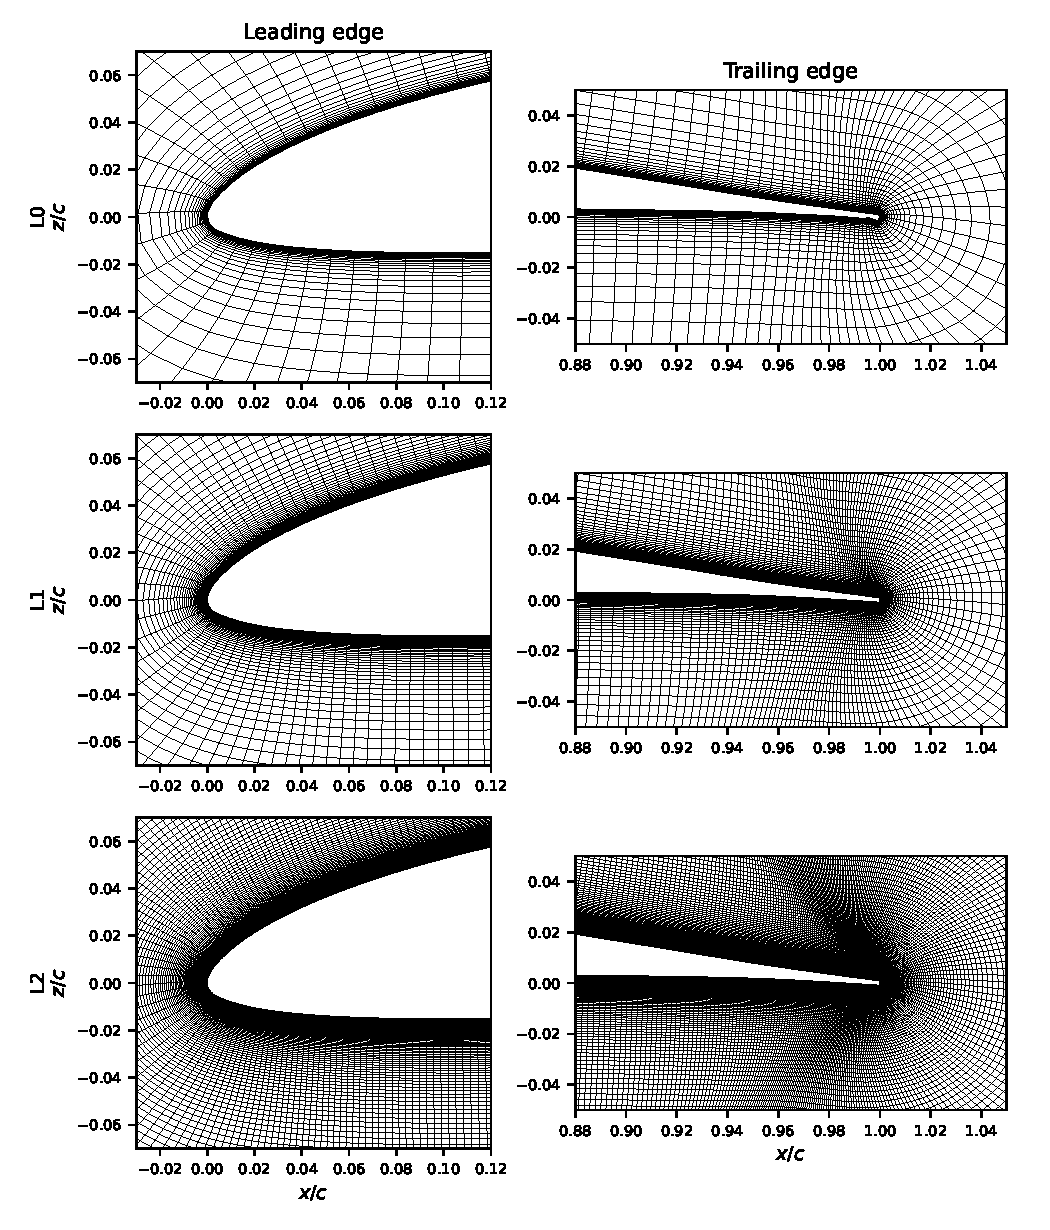
\includegraphics[width=0.9\textwidth]{mesh_eppler_str.pdf}
  \caption{Eppler 387 structured O-grid mesh at the leading edge (left column)
  and trailing edge (right column) for the three refinement levels L0--L2
  (rows), generated by the same recipe as the NLF grid
  (Fig.~\ref{fig:nlfmesh_str}); every length scale halves per level. Chord
  normalized to unity ($z$ vertical).}
  \label{fig:eppmesh_str}
\end{figure}

\begin{figure}[tp]
  \centering
  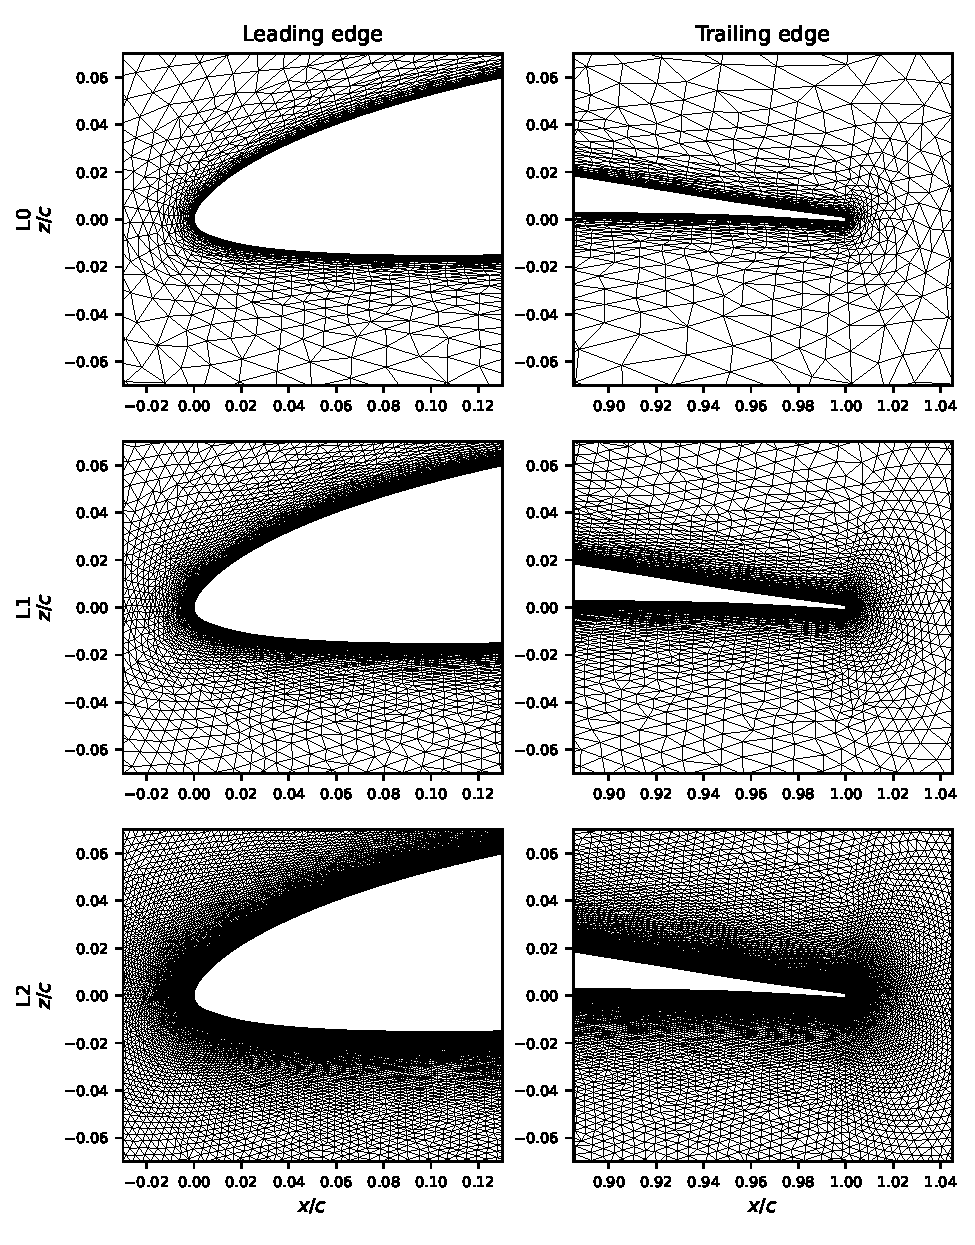
\includegraphics[width=0.9\textwidth]{mesh_eppler_cav.pdf}
  \caption{Eppler 387 unstructured cavity mesh (leading and trailing edges,
  levels L0--L2), built from the same spline contour as the structured grid of
  Fig.~\ref{fig:eppmesh_str} with an anisotropic near-wall boundary-layer
  region; every length scale halves per level.}
  \label{fig:eppmesh_cav}
\end{figure}

\begin{figure}[tp]
  \centering
  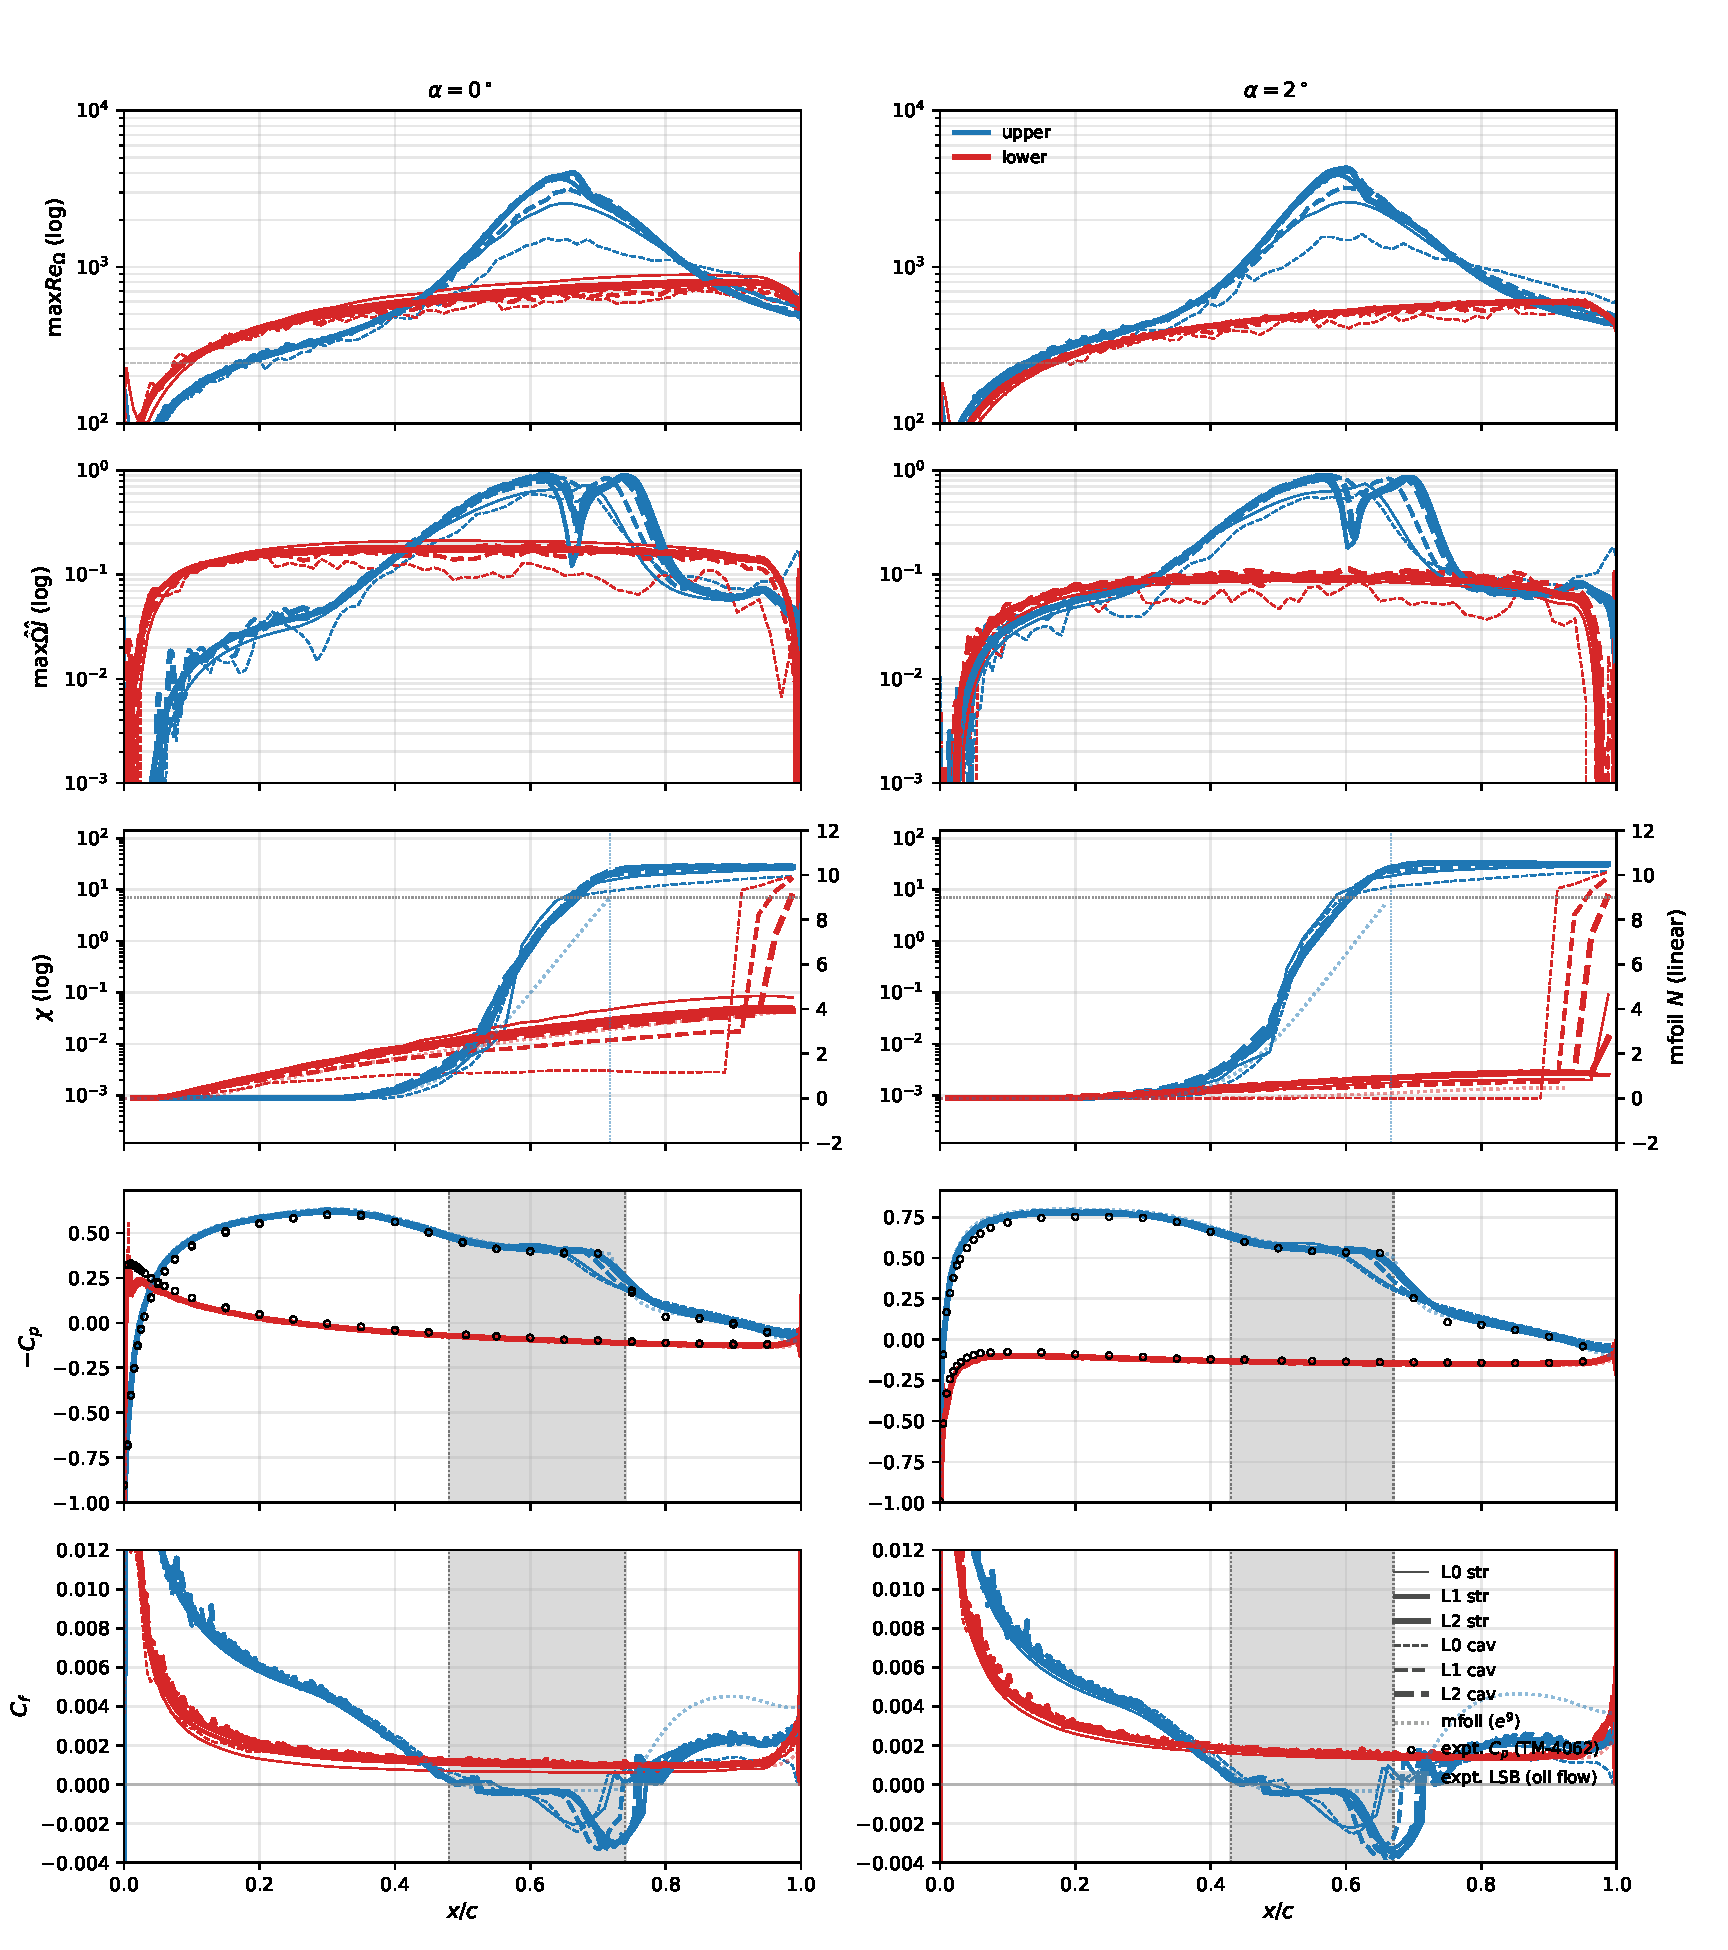
\includegraphics[width=0.86\textwidth]{eppler_cf_lowalpha.pdf}
  \caption{Eppler 387 surface distributions at $\alpha\!\in\!\{0^\circ,2^\circ\}$,
  $Re\!=\!2\!\times\!10^5$, $M\!=\!0.1$, $\chi_\infty\!=\!8.76\!\times\!10^{-4}$
  (matched to $N_\mathrm{crit}\!=\!9$). Five-row layout and line conventions as
  described in the text (row~1 $\max Re_\Omega$, row~2 $\max\Gamma$,
  row~3 $\chi$ with mfoil $N$, row~4 $-C_p$, row~5 signed $C_f$; upper blue /
  lower red, O-grid solid / cavity dashed, L0--L2 by thickness, mfoil $e^9$
  dotted, and the tabulated experimental $C_p$ (NASA TM-4062 App.~D, column with
  the nearest angle of attack) as open black circles on the $-C_p$ row). The signed $C_f$ (row~5) shows the laminar-separation bubble
  directly as the dip below zero on the upper surface. The bubble sits at
  $x/c\!\approx\!0.55$--$0.65$ at $\alpha\!=\!0^\circ$ and marches forward to
  $x/c\!\approx\!0.45$--$0.55$ at $\alpha\!=\!2^\circ$; both Flow360 and mfoil
  show the same recirculation structure.}
  \label{fig:eppcflow}
\end{figure}

\begin{figure}[tp]
  \centering
  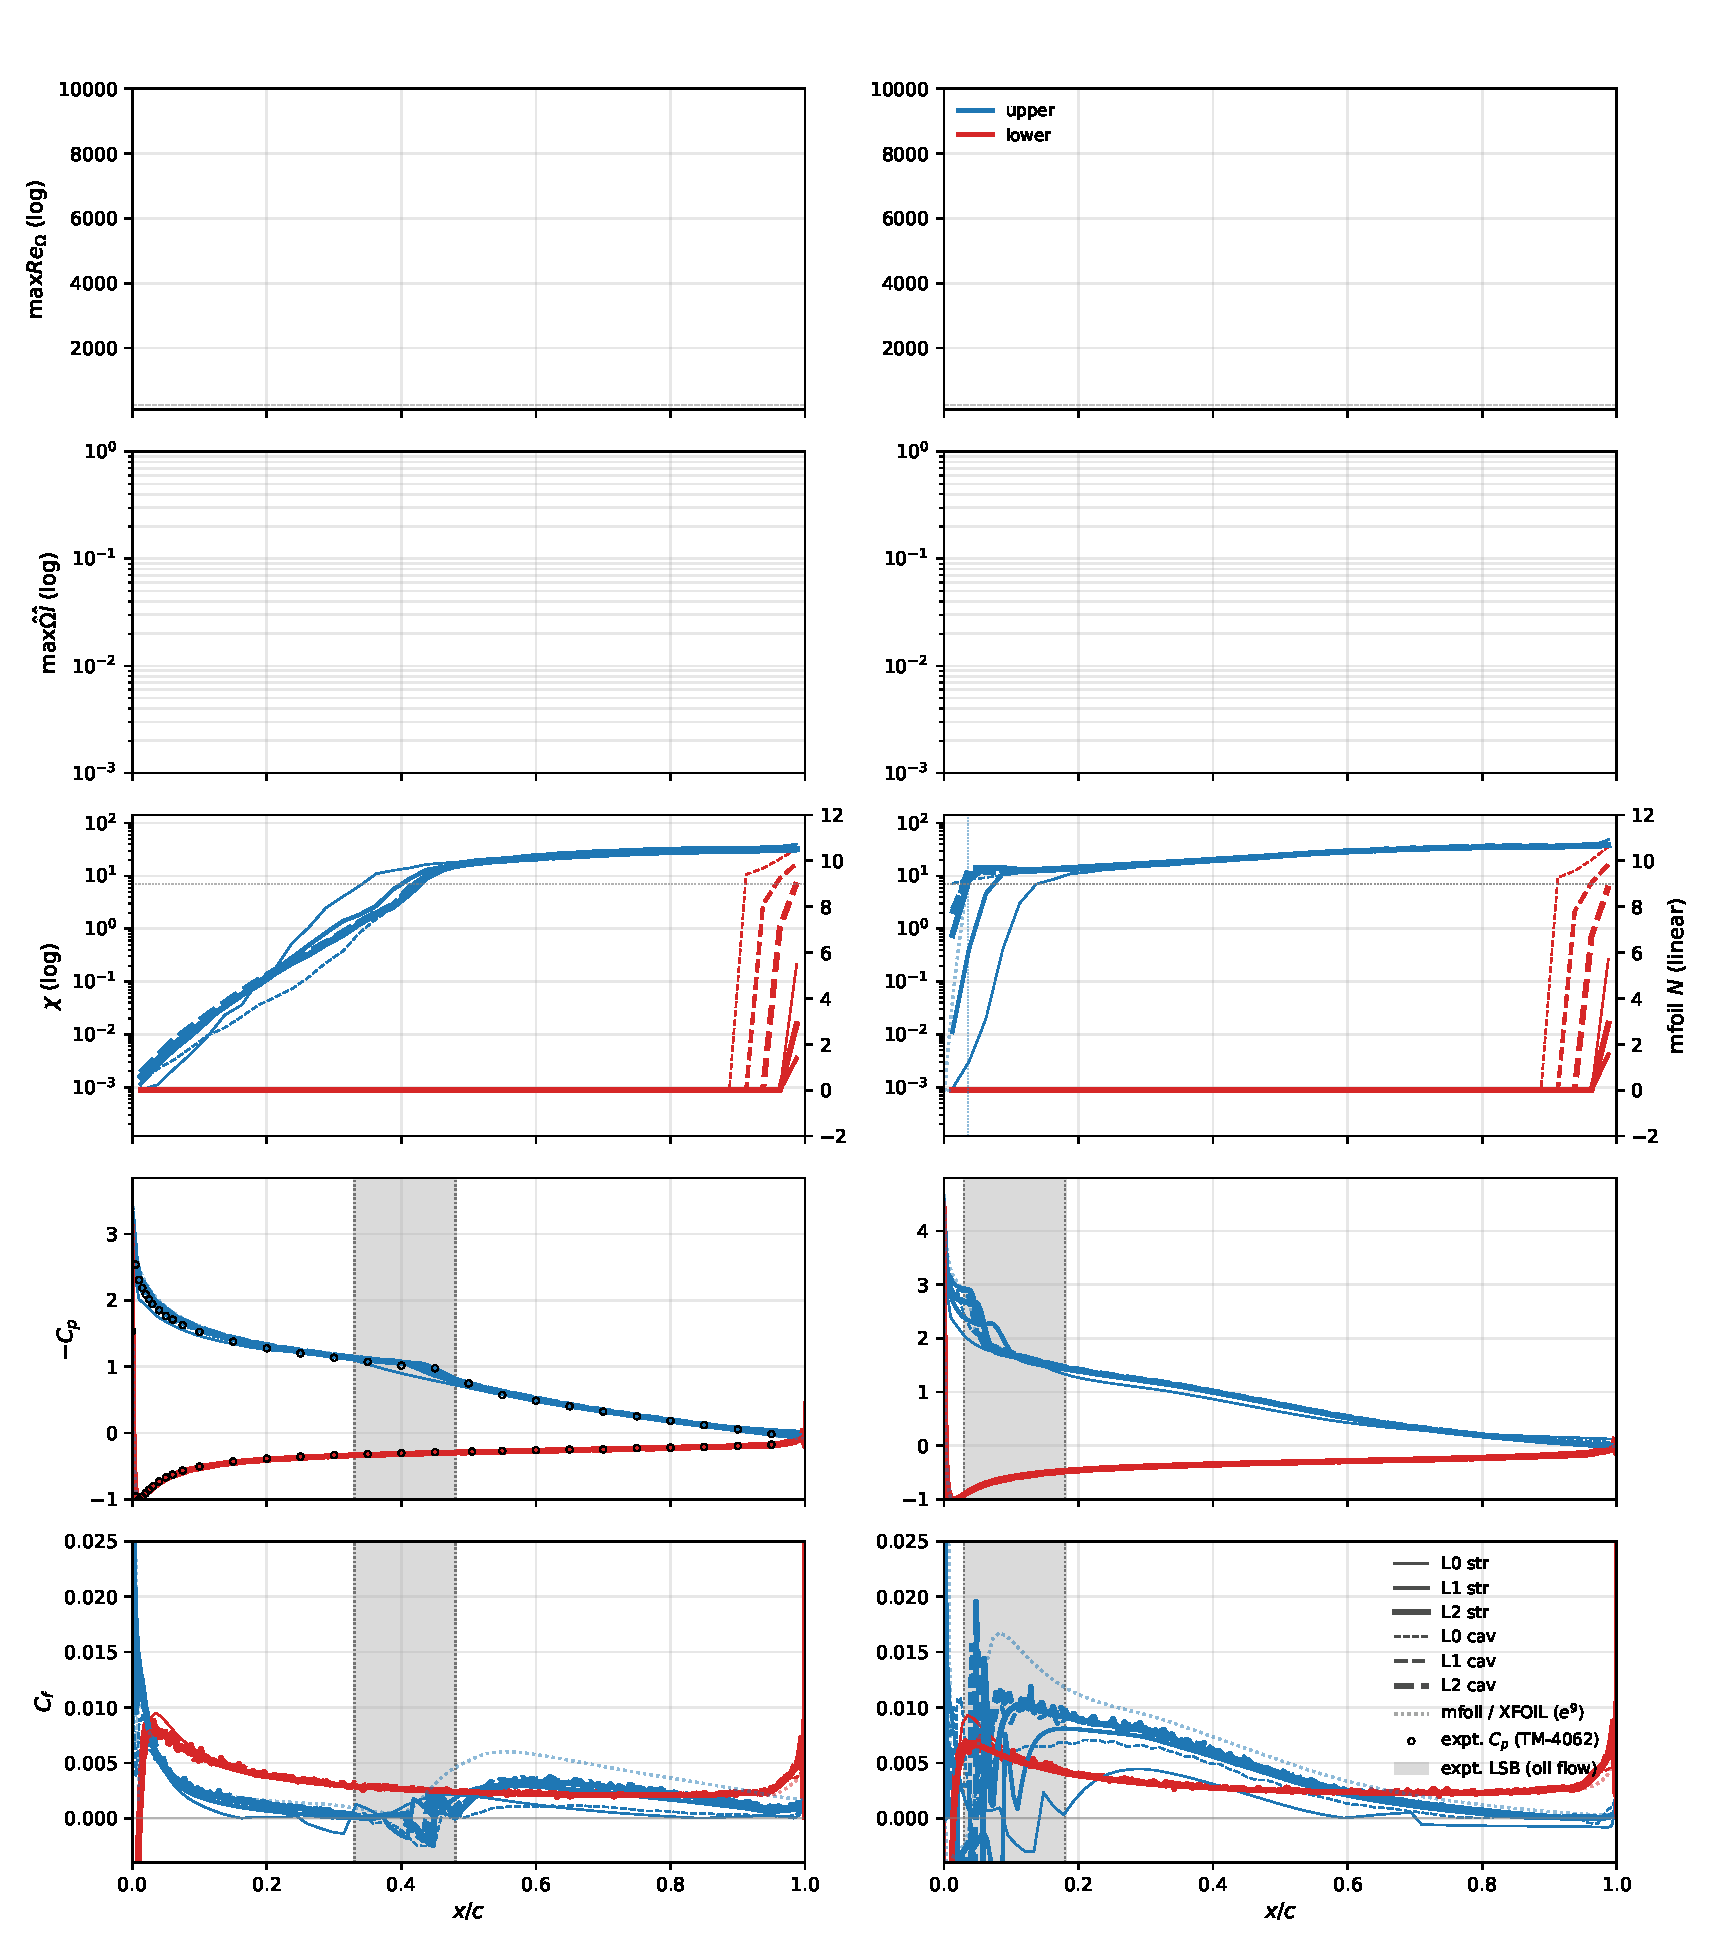
\includegraphics[width=0.86\textwidth]{eppler_cf_highalpha.pdf}
  \caption{As Fig.~\ref{fig:eppcflow}, at $\alpha\!\in\!\{5^\circ,7^\circ\}$.
  At $\alpha\!=\!5^\circ$ the bubble has moved to $x/c\!\approx\!0.40$ and
  shortened; at $\alpha\!=\!7^\circ$ the suction peak is near $-C_p\!\approx\!3$
  and the bubble is at $x/c\!\approx\!0.10$--$0.15$ with a sharp recovery.
  The signed $C_f$ (bottom row) shows the small recirculation directly. The
  lower-surface boundary layer remains attached and essentially laminar to
  $x/c\!\approx\!0.99$ across the entire $\alpha$ range, matching the
  $e^9$ prediction that the lower transition lies aft of the airfoil. At
  $\alpha\!=\!7^\circ$ the dotted reference is XFOIL rather than mfoil, which
  stalls numerically there (Table~\ref{tab:eppxtr}); XFOIL provides $C_p$ and
  $C_f$ only, so the $N$ curve (row~3) is absent at $7^\circ$.}
  \label{fig:eppcfhigh}
\end{figure}

The skin friction (Figs.~\ref{fig:eppcflow}--\ref{fig:eppcfhigh}, bottom rows)
shows the LSB directly: the upper-surface $C_f$ drops below zero in a band
roughly $0.05$--$0.10$ chord wide, then
rises sharply through reattachment and reaches the turbulent level. The signed
$C_f$ is the wall skin friction oriented along the LE$\to$TE surface tangent
(equivalently Flow360's wall-shear-stress vector output, against which we verified
it node-for-node), comparable to mfoil's signed skin friction. Both Flow360
and mfoil show the same recirculation structure at all four incidences and on
both mesh families.

The profile-fullness indicator $\max_y\Gamma$ (row~2 of
Figs.~\ref{fig:eppcflow}--\ref{fig:eppcfhigh}) shows the adverse-gradient
response the Eppler~387 probes: on the upper surface $\Gamma$ climbs from
its attached-layer value $\approx\!1$ through the sigmoid center
$g_c\!=\!1.572$ and saturates at $2$ across the laminar-separation bubble (the
inflectional profile), then relaxes after reattachment, while the lower surface
stays near $\Gamma\!\approx\!1$; the $\Gamma$-sigmoid is what ignites the
amplification at the bubble. The favorable-PG term $\lambda_p$ plays little role
here: at this low Reynolds number the airfoil carries only a short
favorable-gradient segment near the leading edge, so the onset-delay cliff
$Re_\Omega^{\mathrm{c}}(\lambda_p)$ (with the derived $K_\lambda$) transfers
unchanged to the Eppler~387 and leaves the bubble-controlling amplification
untouched.

\begin{table}[tp]
  \centering
  \caption{Upper-surface turbulent-\emph{reattachment} location $x_R/c$ on the
  Eppler 387 at $Re\!=\!2\!\times\!10^5$ across the four incidences, three
  refinement levels, and two mesh families. For a laminar-separation bubble the
  physically observable quantity is the reattachment point, not the amplification
  onset; we define it in the computation as the most-downstream location where the
  signed $C_f$ recovers through $+10^{-3}$ (the return to the turbulent branch aft
  of the bubble), and take the same measure from mfoil's signed $C_f$. \emph{Exp}
  is the oil-flow turbulent reattachment (McGhee et al., NASA TM 4062, Table~III),
  i.e.\ the aft edge of the grey band on the $C_f$ rows of
  Figs.~\ref{fig:eppcflow}--\ref{fig:eppcfhigh}. The lower surface stays attached
  and laminar to the trailing edge at every incidence.}
  \label{tab:eppxtr}
  \begin{tabular}{ccccccccc}
    \toprule
    & \multicolumn{3}{c}{Unstructured cavity} & \multicolumn{3}{c}{Structured O-grid} & & \\
    \cmidrule(lr){2-4} \cmidrule(lr){5-7}
    $\alpha$ & L0 & L1 & L2 & L0 & L1 & L2 & mfoil $e^9$ & Exp (oil flow) \\
    \midrule
    $0^\circ$ & 0.744 & 0.726 & 0.732 & 0.711 & 0.729 & 0.735 & 0.764 & 0.74 \\
    $2^\circ$ & 0.693 & 0.682 & 0.681 & 0.667 & 0.679 & 0.686 & 0.713 & 0.67 \\
    $5^\circ$ & 0.636 & 0.605 & 0.604 & 0.608 & 0.601 & 0.607 & 0.612 & 0.59 \\
    $7^\circ$ & 0.524 & 0.473 & 0.476 & 0.330 & 0.440 & 0.483 & $0.40^\dagger$ & 0.48 \\
    \bottomrule
  \end{tabular}
  \\[2pt]{\footnotesize $^\dagger$mfoil at $\alpha\!=\!7^\circ$ is unreliable
  ($C_l\!=\!0.928$, below its $\alpha\!=\!5^\circ$ value---numerical stall onset);
  the tabulated value is XFOIL's~\cite{drela_xfoil_1989}, which converges cleanly
  there ($C_l\!=\!1.17$). At $\alpha\!\in\!\{0^\circ,2^\circ,5^\circ\}$ XFOIL and
  mfoil agree to within $0.01\,c$.}
\end{table}

The reattachment locations in Table~\ref{tab:eppxtr} converge on both
mesh families: the L1$\to$L2 drift is $\leq\!0.01\,c$ at
$\alpha\!\in\!\{0^\circ,2^\circ,5^\circ\}$, and the two
agree to within $0.007\,c$ at L2 on all four incidences. The
$\alpha\!=\!7^\circ$ case is the most sensitive, as expected near stall---the
structured L0 reattaches $\sim\!0.15\,c$ too early---but at L2 both families
recover $x_R\!\approx\!0.48$. Against the oil-flow data, SA-AI (L2)
matches the measured reattachment to within
$\sim\!0.02\,c$ ($0.73$--$0.74$ vs $0.74$ at $\alpha\!=\!0^\circ$, $0.68$--$0.69$
vs $0.67$ at $2^\circ$, $0.60$--$0.61$ vs $0.59$ at $5^\circ$, and $0.48$ vs
$0.48$ at $7^\circ$), straddling the data. The mfoil $e^9$ reference
reattaches $\sim\!0.02$--$0.04\,c$ downstream of the data at
$\alpha\!\in\!\{0^\circ,2^\circ,5^\circ\}$; at $\alpha\!=\!7^\circ$ mfoil is at the
edge of convergence, so we use XFOIL there (Table~\ref{tab:eppxtr}), which
reattaches at $0.40\,c$, $\sim\!0.08\,c$ ahead of the measured $0.48\,c$.
Reproducing the reattachment---the aft
end of the bubble, set by the post-transition turbulent recovery---to within a
couple percent of chord is the central adverse-pressure-gradient result: the
amplification onset ignites at the front of the bubble, where $\Gamma$ crosses the
sigmoid center, and the modeled turbulent recovery closes it at the measured
station.

\begin{figure}[tp]
  \centering
  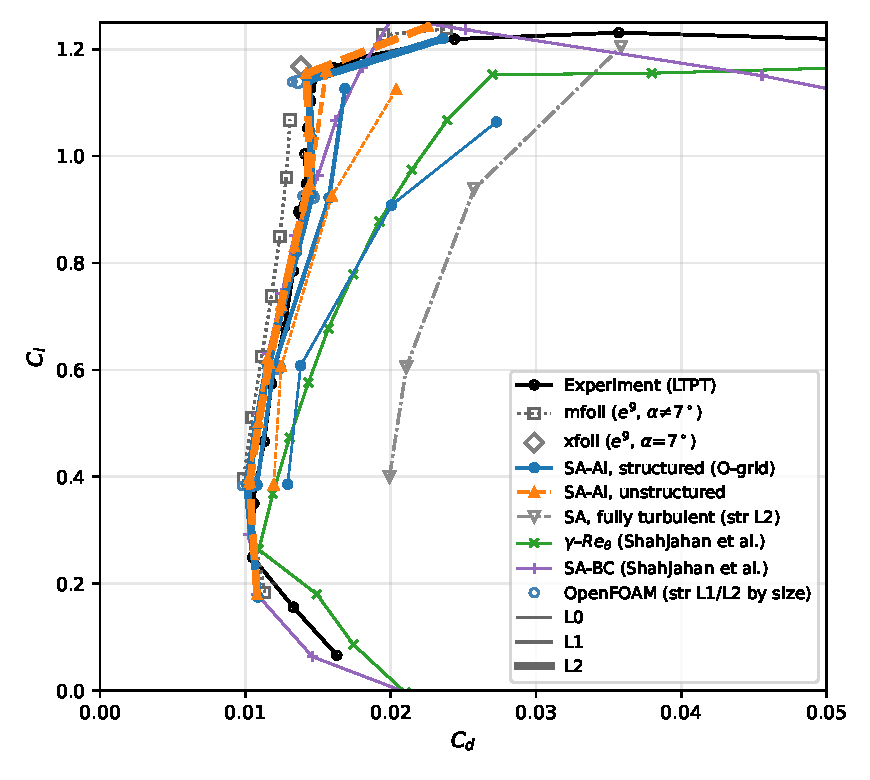
\includegraphics[width=0.62\textwidth]{eppler_polar_compare.pdf}
  \caption{Drag polar of the Eppler 387 at $Re\!=\!2\!\times\!10^5$: the present
  SA-AI prediction (finest structured O-grid and unstructured meshes, L2) at
  $\alpha\!\in\!\{0^\circ,2^\circ,5^\circ,7^\circ\}$ overlaid on the digitized
  experimental section characteristics from the Langley Low-Turbulence Pressure
  Tunnel (McGhee et al., NASA TM-4062, App.~B, $R\!=\!2\!\times\!10^5$) and the
  mfoil $e^9$ reference. The computed points track the low-drag laminar bucket;
  the two mesh families agree to within $\Delta C_d\!\lesssim\!3\times10^{-4}$.
  The grey dash-dot curve is fully turbulent SA ($\chi_\infty\!=\!3$, same
  solver, structured L2 grid), $37$--$50\%$ above the SA-AI drag.}
  \label{fig:epppolar}
\end{figure}

The section drag collapses the bubble physics into a single number.
Figure~\ref{fig:epppolar} overlays the SA-AI polar on the measured section
characteristics: across $\alpha\!\in\!\{0^\circ,2^\circ,5^\circ,7^\circ\}$ the
computed $C_d$ runs $0.0093$--$0.0143$ against the measured $0.0106$--$0.0145$,
so the prediction sits along the left (low-drag) edge of the experimental bucket
and converges onto the data toward $\alpha\!=\!7^\circ$ as the bubble shortens
and the turbulent afterbody grows. The residual low-$\alpha$ offset---a
$\sim\!10$--$15\%$ drag under-prediction---is shared with the mfoil $e^9$
reference, i.e.\ common to both two-dimensional predictions. The structured
O-grid and unstructured meshes bracket the same polar to within
$\Delta C_d\!\lesssim\!3\times10^{-4}$ at L2. Fully turbulent SA on the same
structured L2 grid (grey dash-dot in Fig.~\ref{fig:epppolar}) runs
$C_d\!=\!0.014$--$0.020$ across the four incidences, $37$--$50\%$ above
SA-AI---the price of losing the laminar run and the bubble.

\subsection{Reynolds-number dependence at $\alpha\!=\!5^\circ$}\label{sec:eppresweep}

To assess whether the same constants follow the bubble across the
Reynolds-number range of the McGhee experiment, we hold the incidence at
$\alpha\!=\!5^\circ$ and the freestream seed at
$\chi_\infty\!=\!8.76\!\times\!10^{-4}$ and sweep the four other tabulated
Reynolds numbers,
$Re\!\in\!\{6\!\times\!10^4,\,1\!\times\!10^5,\,3\!\times\!10^5,\,4.6\!\times\!10^5\}$,
reusing the L1 grids of both mesh families from the $Re\!=\!2\!\times\!10^5$
study unchanged (only the reference viscosity changes).
Figures~\ref{fig:eppresweep_low} and~\ref{fig:eppresweep_high} show the resulting
$-C_p$ and signed $C_f$, overlaid with the exact experimental surface pressures
(open circles, from the NASA TM-4062 Appendix~D tables at the column with the
nearest angle of attack) and the mfoil/XFOIL $e^9$ reference where it converges.
All eight solutions are steady and fully converged---the force coefficients are
flat to $\Delta C_l,\Delta C_d\!<\!10^{-8}$ over the final $2000$ iterations,
i.e.\ no bubble limit cycle.

The sweep traces the classic low-$Re$ bubble progression at fixed incidence: as
the Reynolds number rises the transition front moves forward and the
laminar-separation bubble shortens. The upper-surface $C_f$ shows an open,
non-reattaching separation at $Re\!=\!6\!\times\!10^4$---the flow separates near
$x/c\!\approx\!0.35$ and does not recover ahead of the trailing edge, the
low-$Re$ bubble-bursting limit---then a long bubble reattaching near
$x/c\!\approx\!0.72$ at $10^5$, and progressively shorter bubbles reattaching at
$x/c\!\approx\!0.55$ ($3\!\times\!10^5$) and $x/c\!\approx\!0.50$
($4.6\!\times\!10^5$). The section lift, drag, and quarter-chord pitching-moment
coefficients are collected in Table~\ref{tab:eppresweep} against the $e^9$
reference and the tunnel data; the drag falls monotonically across the range,
capturing the sharp low-$Re$ drag rise as the bubble lengthens toward
bursting. The measured
pressures confirm the structure directly: the suction-side plateau of the
separated shear layer appears in the open-circle data at $10^5$ and
$3\!\times\!10^5$ exactly where the computed $C_p$ flattens, and the computed and
measured $C_p$ agree closely on both surfaces at every Reynolds number.

The two mesh families bracket the same solution at the higher
Reynolds numbers ($\Delta C_d\!\lesssim\!4\!\times\!10^{-4}$ at
$3$--$4.6\!\times\!10^5$) and diverge only at $6\!\times\!10^4$, where the open
separation is genuinely mesh-sensitive ($C_l\!=\!0.79$ unstructured vs.\ $0.72$
structured). The experiment itself is bistable there: in the TM-4062 listing at
$Re\!=\!6\!\times\!10^4$, three consecutive repeat points at
$\alpha\!=\!4.00^\circ$ give $c_l\!=\!0.643$, $0.697$, and $0.721$
($c_d\!=\!0.0431$, $0.0386$, $0.0400$), and the measured lift collapses from
$0.838$ at $\alpha\!=\!4.99^\circ$ to $0.639$ at
$\alpha\!=\!5.51^\circ$---run-to-run scatter of the same order as the spread
between the two computed solutions. The mfoil $e^9$ panel reference converges from
$6\!\times\!10^4$ to $3\!\times\!10^5$ but fails at $4.6\!\times\!10^5$
(stagnation-point iteration divergence on the thin high-$Re$ bubble), where
XFOIL~\cite{drela_xfoil_1989} supplies the $e^9$ line
instead. Across the full factor-of-eight Reynolds-number range the model
reproduces the bubble march with the constants of Sec.~\ref{sec:assembled}
untouched.

\begin{table}[tp]
  \centering
  \small
  \setlength{\tabcolsep}{4.5pt}
  \caption{Section coefficients for the Eppler 387 at $\alpha\!=\!5^\circ$
  across the Reynolds sweep: lift, drag, and quarter-chord pitching moment from
  the two L1 mesh families (the same grids as the $Re\!=\!2\!\times\!10^5$
  study), the $e^9$ panel reference (mfoil; XFOIL at $Re\!=\!4.6\!\times\!10^5$,
  where mfoil diverges), and the LTPT measurement (McGhee et al., NASA TM-4062,
  Table~B1, read at the tabulated angle nearest $5^\circ$:
  $\alpha\!=\!4.99^\circ$--$5.06^\circ$). The computed moment is transferred
  from the solver's leading-edge reference to the quarter chord,
  $c_m\!=\!c_{m,\mathrm{LE}}+\tfrac14(c_l\cos\alpha+c_d\sin\alpha)$. Repeat
  experimental points at $Re\!\geq\!10^5$ agree to within $0.006$ in $c_l$ and
  $0.0003$ in $c_d$; at $Re\!=\!6\!\times\!10^4$ the flow is bistable and the
  repeat scatter is an order of magnitude larger (see text).}
  \label{tab:eppresweep}
  \begin{tabular}{l ccc ccc ccc ccc}
    \toprule
    & \multicolumn{3}{c}{SA-AI, structured L1} & \multicolumn{3}{c}{SA-AI, unstructured L1}
    & \multicolumn{3}{c}{$e^9$ panel} & \multicolumn{3}{c}{Exp (LTPT)}\\
    \cmidrule(lr){2-4}\cmidrule(lr){5-7}\cmidrule(lr){8-10}\cmidrule(lr){11-13}
    $Re$ & $c_l$ & $c_d$ & $c_m$ & $c_l$ & $c_d$ & $c_m$ & $c_l$ & $c_d$ & $c_m$ & $c_l$ & $c_d$ & $c_m$ \\
    \midrule
    $6\!\times\!10^4$   & 0.719 & 0.0459 & $-$0.094 & 0.792 & 0.0417 & $-$0.098 & 0.889 & 0.0368 & $-$0.097 & 0.838 & 0.0439 & $-$0.114 \\
    $1\!\times\!10^5$   & 0.895 & 0.0219 & $-$0.082 & 0.914 & 0.0209 & $-$0.085 & 0.952 & 0.0213 & $-$0.087 & 0.873 & 0.0237 & $-$0.089 \\
    $2\!\times\!10^5$   & 0.926 & 0.0137 & $-$0.079 & 0.949 & 0.0133 & $-$0.084 & 0.960 & 0.0128 & $-$0.082 & 0.891 & 0.0138 & $-$0.081 \\
    $3\!\times\!10^5$   & 0.936 & 0.0115 & $-$0.079 & 0.960 & 0.0111 & $-$0.084 & 0.962 & 0.0103 & $-$0.082 & 0.901 & 0.0114 & $-$0.080 \\
    $4.6\!\times\!10^5$ & 0.943 & 0.0100 & $-$0.080 & 0.969 & 0.0096 & $-$0.086 & 0.958 & 0.0085 & $-$0.081 & 0.914 & 0.0093 & $-$0.081 \\
    \bottomrule
  \end{tabular}
\end{table}

\begin{figure}[tp]
  \centering
  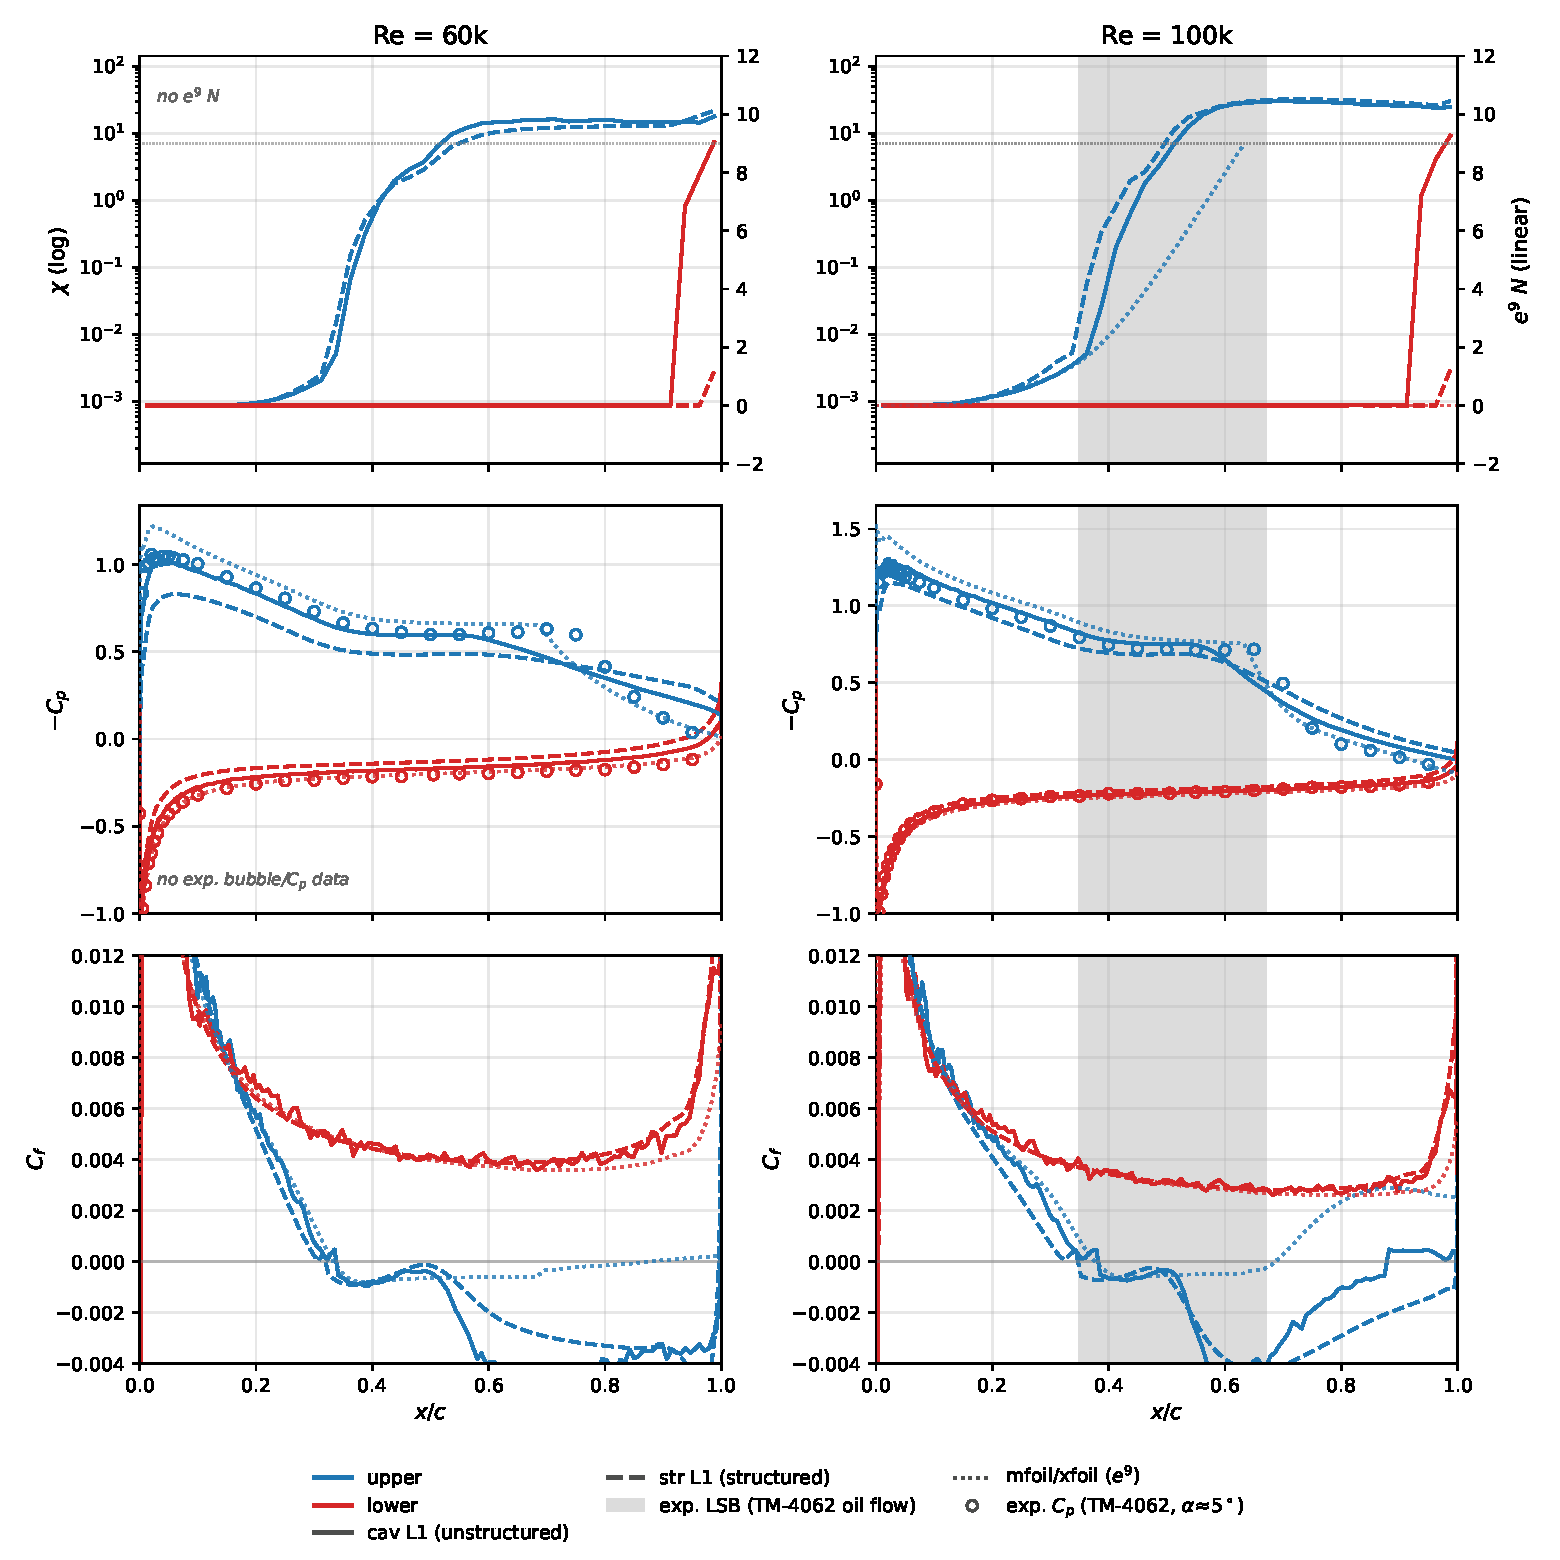
\includegraphics[width=\textwidth]{eppler_L1compare_lowRe.pdf}
  \caption{Eppler 387 at $\alpha\!=\!5^\circ$, $Re\!=\!6\!\times\!10^4$ (left) and
  $1\!\times\!10^5$ (right): the near-wall $\max\chi$ (log, left axis) with the
  mfoil amplification factor $N$ (linear, right axis) where mfoil data exist (top
  row), $-C_p$ (middle row) and signed $C_f$ (bottom row) on the
  L1 grids of both mesh families---unstructured cavity (solid) and structured
  O-grid (dashed), upper surface blue / lower red. Dotted: mfoil $e^9$ reference.
  Open circles: exact experimental surface pressures (NASA TM-4062 Appendix~D,
  column with the nearest angle of attack). Grey band: experimental laminar-separation-bubble
  extent from the oil-flow visualization (TM-4062 Table~III), which exists only at
  $10^5$ among these two; no oil-flow bubble data were taken at $6\!\times\!10^4$.
  At $6\!\times\!10^4$ the upper-surface separation does not reattach ahead of the
  trailing edge (bubble bursting); at $10^5$ a long bubble reattaches near
  $x/c\!\approx\!0.72$.}
  \label{fig:eppresweep_low}
\end{figure}

\begin{figure}[tp]
  \centering
  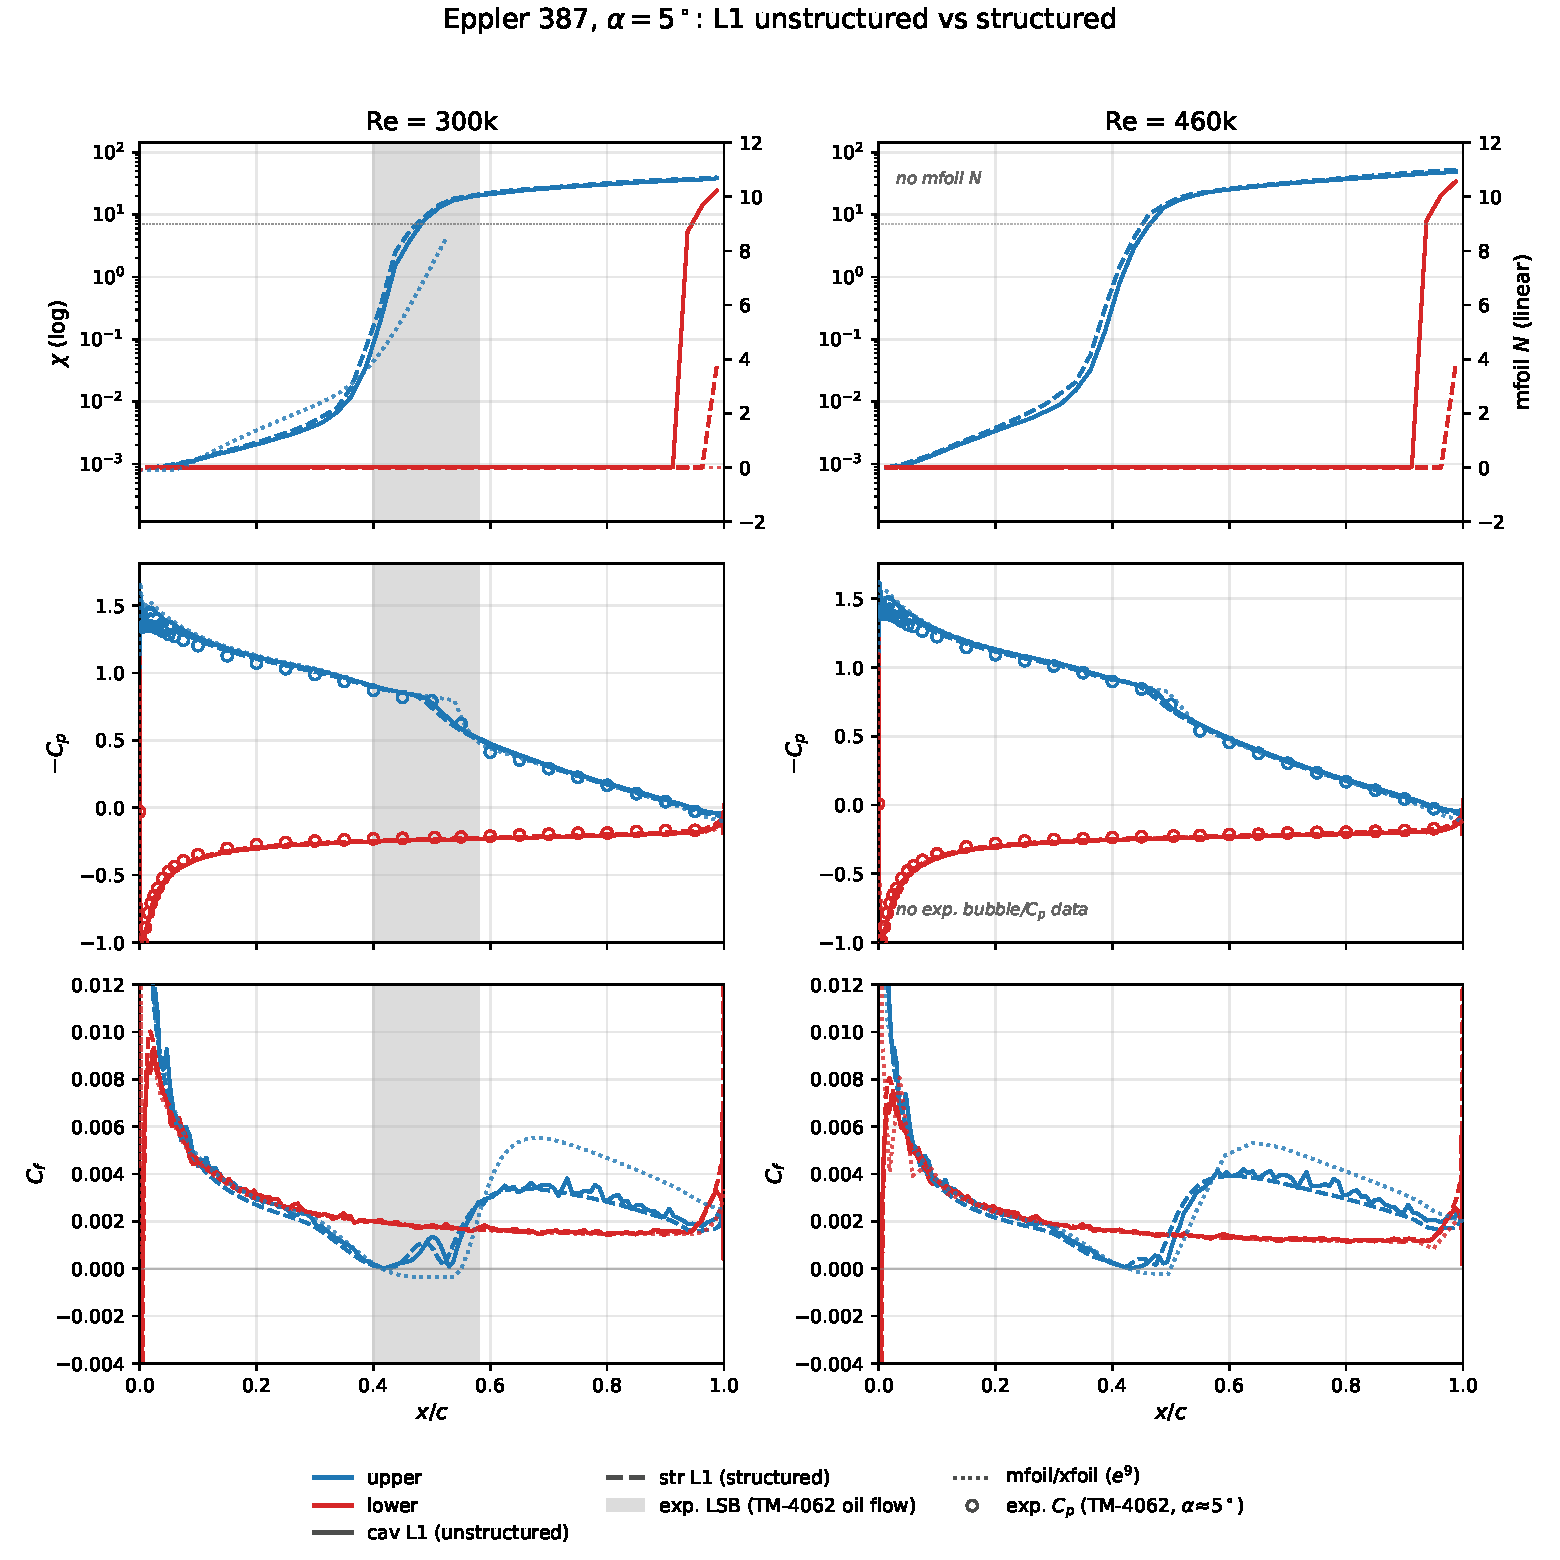
\includegraphics[width=\textwidth]{eppler_L1compare_highRe.pdf}
  \caption{As Fig.~\ref{fig:eppresweep_low}, at $Re\!=\!3\!\times\!10^5$ (left) and
  $4.6\!\times\!10^5$ (right). The bubble is short and moves forward with Reynolds
  number, reattaching near $x/c\!\approx\!0.55$ at $3\!\times\!10^5$ and
  $\approx\!0.50$ at $4.6\!\times\!10^5$. The mfoil $e^9$ panel solver converges at
  $3\!\times\!10^5$ but diverges on the thin bubble at $4.6\!\times\!10^5$, where
  XFOIL supplies the $e^9$ $C_p$/$C_f$ reference (dotted) instead; XFOIL carries no
  amplification envelope, so the $N$ curve (top row, right axis) is drawn only at
  $3\!\times\!10^5$. The oil-flow bubble band is available at $3\!\times\!10^5$ only.}
  \label{fig:eppresweep_high}
\end{figure}

\section{Conclusion}

The Spalart--Allmaras working variable can serve as its own transition
indicator. By replacing the production in the laminar range with a local,
$e^N$-like amplification rate and reverting to standard SA near
$\chi\!\sim\!1$, a single transport equation predicts natural transition
without any auxiliary field.

The amplification rate is anchored to canonical stability limits---the free-shear
rate ($a_{\max}$), the Blasius $e^N$ envelope ($s,g_c$), the critical Reynolds
number ($Re_\Omega^{\mathrm{f}}$), and the favorable-gradient onset delay (the
cliff $Re_\Omega^{\mathrm{c}}(\lambda_p)$, consistent with Drela's
$Re_{\theta c}(H)$)---and then exercised across three
pressure-gradient regimes. The freestream-turbulence
closure $\chi_\infty(Tu)$ is Mack's $e^N$ correlation, and the destruction-gate
width is calibrated so the fully turbulent log law is exactly standard
SA's. On a zero-pressure-gradient flat plate (Sec.~\ref{sec:flatplate}) the Mack
closure places transition onset within $\sim\!10\%$ of the Abu-Ghannam \& Shaw
correlation over the natural-transition range, verifying the Blasius envelope. On
the NLF(1)-0416 at $Re\!=\!4\!\times\!10^6$ (Sec.~\ref{sec:nlfval}) the
favorable-gradient onset-delay slope $K_\lambda$---derived from the Drela--Giles
envelope---places growth onset at the $e^N$ rooftop ignition, and the
handover held across $\alpha\!\in\!\{0^\circ,4^\circ,9^\circ,15^\circ\}$ on
twenty-four cases (both mesh families, three refinement levels). On the Eppler
387 at
$Re\!=\!2\!\times\!10^5$ (Sec.~\ref{sec:eppval}) the
model captured the adverse-gradient, laminar-separation-bubble regime: the signed
skin friction shows the recirculation directly, and transition tracks the $e^N$
reference at the four incidences across another twenty-four cases on the same
two-family ladder; an $\alpha\!=\!5^\circ$ sweep across five Reynolds numbers,
$Re\!=\!6\!\times\!10^4$ to $4.6\!\times\!10^5$, follows the bubble's march and
shortening. The same constants (Sec.~\ref{sec:assembled}) were used
throughout. Across both airfoils the L1$\to$L2 transition-location drift is at
or below $0.01\,c$ away from the marginal cases (the near-LE onset at
$\alpha\!=\!9^\circ$, the slowly-settling NLF lower-surface front, and the
near-stall Eppler $\alpha\!=\!7^\circ$, which reach
$0.03$--$0.05\,c$), and the two independently-generated mesh families agree to
within a few percent of chord.

Several extensions follow. The constants are ballpark values, rounded rather
than optimized (Sec.~\ref{sec:assembled}); a more careful calibration of the
rate---and of the kernel's functional form, adopted for smoothness rather
than derived---against
linear-stability and $e^N$ databases beyond the anchors used here---and a
direct comparison with the algebraic SA-BCM model on community-standard
benchmarks---would establish accuracy beyond the present demonstration.
The out-of-scope regimes noted in the introduction---bypass, crossflow, and
compressible transition---are the natural next steps.

\begin{center}
  \begin{minipage}{0.6\textwidth}\centering
  \begin{CJK}{UTF8}{bsmi}天下萬物生於有，有生於無。\end{CJK}\\[3pt]
  \emph{The myriad things are born of being;\\
  being is born of non-being.}\\[3pt]
  ---\emph{Daodejing}, ch.~40
  \end{minipage}
\end{center}

\section*{Acknowledgments}
The initial idea for this approach was sparked by conversations with Mark Drela
and Philippe R.\ Spalart, whose insights on the amplification-factor envelope
and on the structure of the SA equation were formative.

\bibliography{references}

\end{document}
